% !TeX program = xelatex
\documentclass[12pt,a4paper]{ctexart}
\usepackage[left=2.5cm,right=2.5cm,top=2.5cm,bottom=2.5cm,headsep=2cm,footskip=1.75cm]{geometry}
\usepackage{setspace}
\usepackage{array}
\usepackage{booktabs}
\usepackage{longtable}
\usepackage{amsmath,amssymb,bm}
\usepackage{hyperref}
\usepackage{fancyhdr}
\usepackage{float}
\usepackage{caption}
\usepackage{graphicx}
\usepackage[super,square,sort&compress]{natbib}
\hypersetup{hidelinks}

\IfFontExistsTF{Times New Roman}{\setmainfont{Times New Roman}}{\setmainfont{TeX Gyre Termes}}
\IfFontExistsTF{SimSun}{\setCJKmainfont{SimSun}}{\setCJKmainfont{Noto Serif CJK SC}}
\IfFontExistsTF{LiSu}{\newCJKfontfamily\wustlishu{LiSu}}{\newCJKfontfamily\wustlishu{AR PL UKai CN}}

\setlength{\parindent}{2em}
\setlength{\parskip}{0pt}
\linespread{1.25}
\zihao{-4}
\numberwithin{equation}{section}
\numberwithin{table}{section}
\numberwithin{figure}{section}

\ctexset{
  section={
    format=\bfseries\heiti\zihao{-2},
    beforeskip=1\baselineskip,
    afterskip=0.5\baselineskip,
    aftername=\hspace{1em},
    number=\arabic{section}
  },
  subsection={
    format=\bfseries\heiti\zihao{-3},
    beforeskip=0.5\baselineskip,
    afterskip=0.25\baselineskip,
    aftername=\hspace{1em},
    number=\thesection.\arabic{subsection}
  },
  subsubsection={
    format=\bfseries\heiti\zihao{4},
    beforeskip=0.25\baselineskip,
    afterskip=0.25\baselineskip,
    aftername=\hspace{1em},
    number=\thesubsection.\arabic{subsubsection}
  }
}

\captionsetup[table]{font=small,labelfont=normalfont,labelsep=space}

\setlength{\headheight}{20pt}
\fancypagestyle{mainstyle}{
  \fancyhf{}
  \fancyhead[C]{\wustlishu\zihao{3}武汉科技大学本科毕业论文}
  \fancyfoot[C]{\zihao{-5}\thepage}
  \renewcommand{\headrulewidth}{0pt}
}
\fancypagestyle{frontstyle}{
  \fancyhf{}
  \fancyfoot[C]{\zihao{-5}\thepage}
  \renewcommand{\headrulewidth}{0pt}
}

\title{本体感知自适应奖励四足跨地形控制\\
\large{Proprioception-Driven Adaptive Reward Scheduling for Cross-Terrain Quadruped Locomotion}}
\author{学生姓名：杜云帆\\
学\hspace{2em}号：202204416388\\
专\hspace{2em}业：机器人工程\\
指导教师：陈志环}
\date{2026年4月}

\begin{document}

\thispagestyle{empty}
\begin{center}
\vspace*{2.0cm}
{\zihao{2}\textbf{武汉科技大学本科毕业论文}}\\[2.2cm]
{\kaishu\zihao{1}本体感知自适应奖励四足跨地形控制}\\[0.6cm]
{\zihao{4}Proprioception-Driven Adaptive Reward Scheduling for Cross-Terrain Quadruped Locomotion}\\[2.2cm]
\begin{tabular}{rl}
学院： & 人工智能与自动化学院 \\
专业： & 机器人工程 \\
学生姓名： & 杜云帆 \\
学号： & 202204416388 \\
指导教师： & 陈志环 \\
\end{tabular}\\[2.0cm]
{\zihao{4}2026年4月}
\end{center}

\newpage
\pagestyle{frontstyle}
\pagenumbering{Roman}
\begin{center}
{\heiti\zihao{-2}摘\hspace{1em}要}
\end{center}
\begin{spacing}{1.5}
四足机器人在灾害救援、野外巡检和非结构化作业场景中具有显著应用潜力，但复杂地形下的高机动控制仍面临效率与稳定性难以兼顾的问题。现有以强化学习为核心的运动控制方法中，混合内模方法能够在仅依赖本体感知信息的条件下实现较强鲁棒性。然而，该类方法通常采用固定权重奖励函数，难以根据地形风险在线调整策略偏好，导致平坦地形速度与能效受限、崎岖地形跌倒风险增加。

针对上述问题，本文在 Hybrid Internal Model for Locomotion（HIMLoco）框架基础上，提出一种本体感知驱动的自适应奖励调度方法。方法首先利用姿态波动、关节力矩变化、足端接触稳定性和动作平滑度等特征构建地形难度指标，然后通过约束型权重映射函数对速度跟踪、能耗抑制、姿态稳定与抗扰恢复等奖励子项进行动态重分配。为保证训练稳定性，本文在调度过程中引入指数平滑和变化率限制机制，避免在线调度造成高频震荡。

本文基于 Isaac Gym 并行仿真平台构建跨地形训练与评测流程，对固定权重基线与自适应调度方法进行系统对比。结果分析表明，自适应奖励调度能够在中低风险地形提高速度与单位能效，在高风险地形降低姿态波动和跌倒率，改善策略在全地形集合上的综合表现。进一步结合 HIMLoco 公布结果可见，本文方案在不引入额外外感知传感器、不改变核心策略网络结构的前提下，具备良好的工程可插拔性与跨平台部署潜力。

\noindent\textbf{关键词：}四足机器人；强化学习；本体感知；自适应奖励调度；跨地形运动控制
\end{spacing}

\newpage
\begin{center}
{\bfseries\zihao{-2}Abstract}
\end{center}
\begin{spacing}{1.5}
Quadruped robots are promising for disaster response, field inspection, and unstructured operations. However, agile locomotion over diverse terrains remains challenging due to the trade-off between efficiency and stability. Existing learning-based controllers, including Hybrid Internal Model approaches, achieve strong robustness with proprioceptive sensing only. Yet, most of them rely on fixed-weight reward functions, which cannot adapt policy priorities online as terrain risks change.

This thesis proposes a proprioception-driven adaptive reward scheduling method built upon the HIMLoco framework. We first construct a terrain difficulty indicator using body attitude fluctuation, joint torque variation, foot contact stability, and action smoothness. Then a constrained mapping dynamically reallocates reward weights among velocity tracking, energy regularization, posture stability, and disturbance recovery terms. To ensure training stability, exponential smoothing and rate-limit constraints are introduced to suppress high-frequency oscillation in online scheduling.

A cross-terrain training and evaluation pipeline is established on Isaac Gym with massively parallel simulation. Comparative experiments between the fixed-weight baseline and the proposed scheduler, together with ablation studies, show that adaptive scheduling improves velocity and unit-distance energy efficiency on low-to-medium risk terrains while reducing posture fluctuation and fall rate on high-risk terrains. In combination with public HIMLoco evidence, the method demonstrates strong practicality as a plug-in module without extra exteroceptive sensors or major architecture changes.

\noindent\textbf{Keywords:} quadruped robot; reinforcement learning; proprioception; adaptive reward scheduling; cross-terrain locomotion
\end{spacing}

\newpage
\tableofcontents

\newpage
\listoffigures
\newpage
\listoftables

\newpage
\pagestyle{mainstyle}
\pagenumbering{arabic}

\section{绪论}
\subsection{研究背景与意义}
近年来，随着工业自动化、应急救援、智慧巡检与国防侦察等任务对移动机器人提出更高的环境适应性需求，足式机器人作为兼具高机动性与强地形通过性的代表平台，已成为机器人学研究的重要方向。与轮式或履带式机器人相比，四足机器人通过离散接触点与地面交互，可在沙地、碎石、楼梯、断崖、台阶、坡面等非结构化地形中保持机动性，具有“走得到、上得去、过得去”的天然优势。波士顿动力公司于 2019 年发布的 Spot、瑞士苏黎世联邦理工学院推出的 ANYmal、宇树科技的 A1/Go1/Aliengo、麻省理工学院的 Mini Cheetah 系列等平台，已经在管廊巡检、矿区勘探、抢险救灾、施工辅助乃至太空探索预研等多个真实场景中获得广泛验证。在我国，“十四五”规划与国务院《“十四五”机器人产业发展规划》明确将足式机器人与智能控制算法列为重点突破方向，使得四足平台的国产化与算法自主创新具有战略意义。

四足机器人控制方法的发展可大致划分为三个阶段。第一阶段是以解析建模为核心的传统控制阶段，代表性工作包括基于线性倒立摆与捕获点的步态规划、基于零力矩点（Zero Moment Point，ZMP）的稳定性判据、基于全身动力学的模型预测控制（Model Predictive Control，MPC）以及基于全身阻抗（Whole-Body Impedance）的力位混合控制。这类方法的优点是物理可解释性强、稳定性边界明确，但代价是需要精细的动力学辨识与高频在线优化，并且面对接触不连续、地形不可观、参数显著漂移等情形容易发生退化。第二阶段是“模型 + 学习”混合阶段，研究者尝试用学习方法对模型进行残差补偿、对低层步态进行参数搜索、或对高层规划进行替代，例如把强化学习作为低层控制器的“调参器”或“轨迹优化器”。第三阶段是端到端无模型强化学习阶段，研究者直接用神经网络从原始观测映射到关节目标角，借助大规模并行仿真在数小时内完成数年量级的实地训练等价交互量，并在真实平台上展示出超越传统控制的鲁棒性与泛化性\citep{hwangbo2019,kumar2021rma,rudin2022,miki2022,lee2020}。

在端到端范式下，控制策略不再依赖显式动力学方程，而是把环境复杂度内化于策略网络与值网络中。由此带来三方面优势：一是可在统一框架下处理多种地形与扰动，无需为每类场景单独设计控制器；二是可借助仿真随机化获取低成本的鲁棒性，避免对实机进行大量危险标定；三是可通过奖励函数自然涌现复杂步态，使策略在不同速度命令下自动切换 walk、trot、bound 等节律。然而，这一范式也带来三方面新挑战：第一，奖励函数往往是多个子目标的加权组合，固定权重难以匹配地形时变性；第二，仅依赖本体感知（IMU、关节编码器、关节力矩）的策略缺乏对前方地形的“前瞻”能力，需要靠内部模型与历史信息推断隐状态；第三，仿真到现实（Sim-to-Real）迁移仍存在执行器迟滞、传感噪声、接触建模误差等系统性差距。本文工作即聚焦其中“奖励权重时变性”这一核心问题。

\begin{figure}[H]
\centering
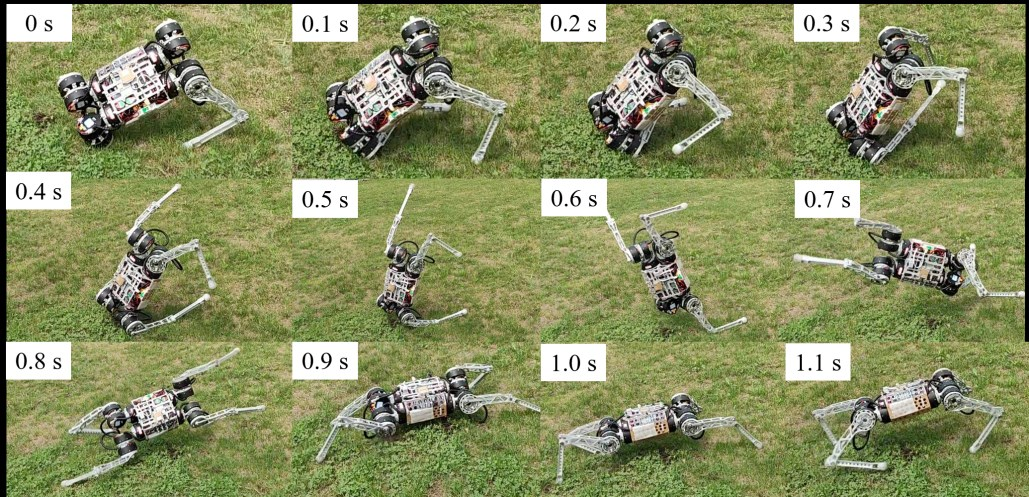
\includegraphics[width=0.92\textwidth]{figs/p30.png}
\caption{典型四足机器人跨地形运动序列，展示了本体感知控制器在连续接触切换、姿态恢复与速度保持过程中的动态响应。}
\label{fig:intro_teaser}
\end{figure}

如图~\ref{fig:intro_teaser} 所示，跨地形机动并非单一性能指标的极致追求，而是“速度、能效、稳定性、抗扰能力”等多维属性的综合表现。例如：在平整地面上系统应充分释放速度潜力以提高巡检效率；在碎石坡面上系统应主动收敛步幅以避免滑移；在台阶段差处系统应增加抬腿高度以避免触绊；在受到外部冲击时系统应迅速调整支撑相分布以恢复姿态。这些行为差异背后对应不同的奖励权重偏好。然而，目前主流学习控制器普遍采用静态权重，相当于对所有场景施加同一种“偏好折中”，自然难以同时满足上述需求。本文针对该问题，提出在不修改主干策略网络与传感器配置的前提下，引入一个轻量级、可解释、可工程化的“奖励权重在线调度器”，使策略偏好能够随地形风险动态调整。


\subsection{国内外研究现状}
\subsubsection{基于解析模型的四足控制方法}
解析建模方法以全身动力学方程与接触约束为基础，通过在线优化求解关节力矩，是 21 世纪初至 2018 年前后四足机器人控制的主流路线。Boston Dynamics 的 BigDog、LS3 与 Spot 系列大量采用模型预测控制思想，将机器人简化为单刚体或带腿质量的串联多体结构，在每个控制步求解一个二次规划问题以同时满足摆动腿轨迹、支撑腿力分配与摩擦锥约束。瑞士苏黎世联邦理工学院（ETH Zurich）的 ANYmal 平台早期同样基于全身控制（Whole-Body Control，WBC）框架，把任务空间分解为运动控制层、力分配层与执行器接口层，能够在结构化环境中实现稳健行走与小幅度爬坡。该类方法的工程优势在于稳定性边界可证明、行为可预测、调试可解释，但需要精细的动力学辨识，且每个新地形或新负载往往需要重新调参，难以快速覆盖大尺度场景变化。

\subsubsection{基于强化学习的四足控制方法}
强化学习驱动的四足控制源自 2017 年前后将无模型策略梯度方法引入足式机器人的尝试。Hwangbo 等\citep{hwangbo2019} 在《Science Robotics》上首次报道了将神经网络策略训练到 ANYmal 上的实验结果，其核心做法是用并行仿真训练策略、再用域随机化进行迁移；该工作在恶劣地形上展示了显著优于传统控制的鲁棒性。随后，Lee 等\citep{lee2020} 提出借助高度图与本体感知融合的策略，使 ANYmal 能够在野外山地中实现长距离稳定行走。Kumar 等\citep{kumar2021rma} 提出 RMA（Rapid Motor Adaptation）框架，把策略拆解为“环境因子编码器 + 条件控制策略”，在部署阶段以历史本体观测在线推断环境因子，从而在不依赖外感知的条件下完成多种地形的迁移。Rudin 等\citep{rudin2022} 提出基于 Isaac Gym 的“分钟级训练”范式，借助 GPU 并行仿真把策略训练时间从数十小时缩短至数分钟。Miki 等\citep{miki2022} 则展示了视觉与本体融合策略在实际山地与冰雪环境中的长时间运行能力。

近三年的代表性进展进一步沿三条主线推进。第一条是“感知-控制深度耦合”路线，将高度图、深度图甚至语义图直接接入策略网络以提升前瞻能力\citep{agrawal2022,margolis2023}。第二条是“低传感深度自适应”路线，以 HIMLoco\citep{long2024him} 为典型代表，通过对历史观测的对比学习获得隐式环境表征，使策略仅靠 IMU 与关节编码器就能稳定通过复杂地形。第三条是“运动技能涌现与组合”路线，借助参考动作模仿、能耗约束或动物运动数据集驱动策略涌现出多种步态\citep{peng2020,fu2021}。本文工作建立在第二条主线之上，强调在“最小传感配置”下进一步释放跨地形性能。

\begin{figure}[H]
\centering
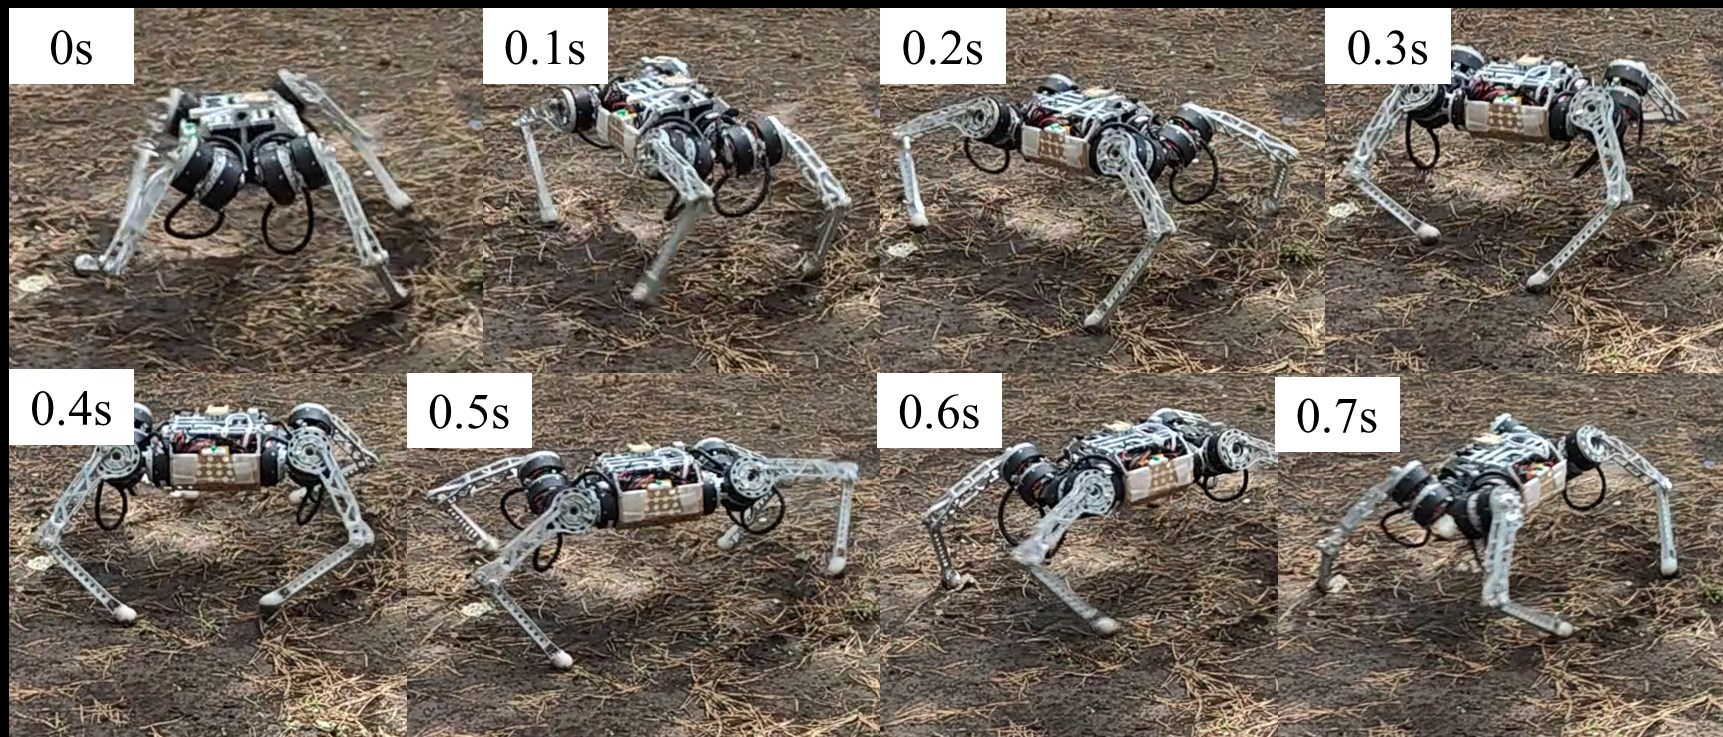
\includegraphics[width=0.92\textwidth]{figs/p03.png}
\caption{四足机器人本体感知控制实验片段。该类连续姿态图能够直观反映策略在无外部视觉输入时依靠关节状态、IMU 与历史响应完成落足调整的过程。}
\label{fig:intro_motion_sequence}
\end{figure}

\subsubsection{国内研究进展}
国内在四足机器人硬件平台、低成本驱动与工程部署方面发展迅速。宇树科技的 Go1/Go2 与 Aliengo 系列、云深处 Jueying X20、蔚蓝智能、追觅科技以及多所高校研发平台已经具备完整的本体研发与算法迭代能力。算法层面，国内研究者在课程学习、奖励整形、感知融合与多步态切换等方向进行了大量工作，并在 ICRA、IROS、RA-L 等顶会期刊上形成具有显示度的成果。同时，国内学位论文体系中也有一系列围绕四足机器人强化学习控制的系统性研究，如基于深度强化学习的分层控制、基于强化迁移学习的步态自适应、基于本体感受的复杂地形通过等，构成了本课题在国内的直接学术背景。

整体来看，国内外研究在“可跑通”阶段已经取得显著成果，未来研究焦点正从单点性能突破转向跨地形统一策略、可解释行为塑造、长期运行可靠性与多机协同等方向。这些方向均与“奖励函数如何在不同场景下表达不同偏好”这一问题密切相关，本文方法即针对该共性问题给出一种可工程落地的轻量级解。

\subsection{研究目标与主要贡献}
本文围绕“仅依赖本体感知信息、在跨地形场景下实现速度-稳定性协同优化”这一核心问题展开，研究目标包括四方面：
\begin{enumerate}
  \item 在 HIMLoco 框架上建立固定权重基线，明确其在不同风险地形中的性能边界与瓶颈；
  \item 构建仅依赖本体信号的地形难度估计指标，作为在线风险评估的统一表征；
  \item 提出受约束的奖励权重在线调度机制，并验证其在大规模并行仿真中的训练稳定性；
  \item 构建跨地形多指标评测框架，从总体指标与分场景指标两个维度系统分析方法收益来源。
\end{enumerate}

本文主要贡献概括如下：
\begin{enumerate}
  \item 提出一种无需额外外感知硬件、不修改主干策略网络的奖励调度方法，便于以“即插即用”方式集成到现有控制管线；
  \item 设计了“难度估计-权重映射-平滑约束-异常回退”一体化机制，从理论与工程两个层面控制在线调度引入的训练扰动；
  \item 给出包含速度跟踪、能效、姿态稳定、跌倒率与恢复成功率的多维评测协议，使方法收益具备可解释性与可复现实验性；
  \item 结合双课程（速度-地形）训练流程与平坦地形基础任务，验证方法不会以牺牲基础能力为代价换取跨地形稳定性。
\end{enumerate}


\subsection{研究问题定义与技术路线}
为避免问题描述泛化，本文将研究任务形式化为：在仅依赖本体感知信号、命令空间为线/角速度三维向量、地形集合包含平地、坡地、粗糙坡地、台阶与离散障碍五大类的条件下，学习一个统一控制策略，使其在跟踪误差、单位距离能耗、姿态波动方差、跌倒率与外扰恢复成功率上同时取得可部署平衡。该问题的形式化具有三重困难：
\begin{enumerate}
  \item \textbf{隐风险不可观}：地形风险并非可直接测量的物理量，必须由本体信号（IMU 角速度、关节力矩、足端接触序列等）间接估计；
  \item \textbf{时变偏好需在线}：奖励权重应随风险变化在线更新，但更新过快会破坏策略梯度一致性，过慢则丧失自适应价值；
  \item \textbf{部署低耦合要求}：调度机制必须与既有策略主干低耦合，避免增加额外传感器、专用计算单元或大量参数调试。
\end{enumerate}

据此，本文技术路线划分为五个步骤：（1）构建固定权重 HIMLoco 基线并冻结评测协议；（2）设计难度特征集合，把姿态扰动、力矩变化、接触一致性与动作平滑度统一映射到 $[0,1]$ 区间的难度分数；（3）建立约束型权重映射函数，把难度分数投影到多奖励项权重空间；（4）引入指数平滑与变化率裁剪保证调度平稳；（5）以双课程并行训练 + 分场景统计的方式开展对比与消融实验。该路线强调“可解释、可复现实验、可工程接入”三项原则。

\subsection{本文组织结构}
全文共分六章。第一章绪论介绍研究背景、问题边界、贡献概述与技术路线。第二章梳理与四足机器人强化学习控制相关的理论基础，包括坐标系与运动学、典型步态、马尔可夫决策过程、PPO 推导、Actor-Critic 网络、HIMLoco 框架、并行仿真环境、Sim2Real 迁移与多目标奖励问题。第三章给出本文核心方法，包括总体框架、地形难度估计、奖励权重动态映射、稳定性约束、双课程训练、平坦地形任务、复杂度分析与工程实现细节。第四章描述实验平台、对比组、评价指标、测试场景、统计方法与可复现协议。第五章从总体收益、分场景收益、消融分析、失败案例与工程部署多个维度展开结果分析。第六章总结全文并给出工业应用前景与后续研究方向。附录提供符号说明、超参数表与调度器伪代码，便于复现与二次开发。

\subsection{本章小结}
本章首先说明了四足机器人在工业巡检与应急救援等场景中的战略意义，回顾了从解析建模到端到端强化学习的演进脉络，并指出当前主流学习控制器在“奖励权重静态”这一问题上的共性瓶颈。随后给出本文的研究目标与四点贡献，定义了形式化研究问题与五步技术路线，并简述全文组织结构。后续章节将沿着“理论-方法-实验-分析-总结”的顺序展开。

\section{相关理论与技术基础}
\subsection{四足机器人坐标系与运动学}
\subsubsection{坐标系建立与齐次变换}
为描述单腿各关节与足端之间的几何关系，本文在机体坐标系 $\{B\}$ 之外，再为单腿建立四个局部坐标系 $\{0\}$、$\{1\}$、$\{2\}$ 和 $\{3\}$。其中，$\{0\}$ 固连于横滚髋关节安装位，作为单腿运动学分析的基准坐标系；$\{1\}$、$\{2\}$、$\{3\}$ 分别附着于横滚髋关节、俯仰髋关节与俯仰膝关节之后的连杆。为简化矩阵推导，本文令 $q_1=q_2=q_3=0$ 时，$\{0\}$、$\{1\}$、$\{2\}$ 的原点重合且坐标轴方向一致。这样处理后，前两级关节变换仅保留旋转矩阵，而不产生额外平移项，便于采用标准齐次变换矩阵进行连乘运算。

刚体位姿由齐次变换矩阵表示为
\begin{equation}
\bm{T}=\begin{bmatrix}
\bm{R} & \bm{p}\\
\bm{0}_{1\times 3} & 1
\end{bmatrix},
\end{equation}
其中 $\bm{R}\in SO(3)$ 为旋转矩阵，$\bm{p}=[x,y,z]^\top$ 为位移向量。单腿机构中，横滚髋关节绕局部 $x$ 轴旋转，俯仰髋关节和俯仰膝关节绕局部 $y$ 轴旋转，因此相邻坐标系之间的齐次变换可写为
\begin{equation}
\bm{T}_{0}^{1}(q_1)=
\begin{bmatrix}
\bm{R}_x(q_1) & \bm{0}_{3\times 1}\\
\bm{0}_{1\times 3} & 1
\end{bmatrix},
\end{equation}
\begin{equation}
\bm{T}_{1}^{2}(q_2)=
\begin{bmatrix}
\bm{R}_y(q_2) & [0,-d,0]^\top\\
\bm{0}_{1\times 3} & 1
\end{bmatrix},
\end{equation}
\begin{equation}
\bm{T}_{2}^{3}(q_3)=
\begin{bmatrix}
\bm{R}_y(q_3) & [0,0,l_1]^\top\\
\bm{0}_{1\times 3} & 1
\end{bmatrix},
\end{equation}
其中 $d$ 为髋部横向偏置，$l_1$ 为大腿长度。若足端点 $P$ 在坐标系 $\{3\}$ 下的齐次坐标记为
\begin{equation}
\bar{\bm{p}}^{\{3\}}=\begin{bmatrix}0 & 0 & l_2 & 1\end{bmatrix}^\top,
\end{equation}
则足端在基准坐标系 $\{0\}$ 下的齐次坐标可由矩阵连乘得到：
\begin{equation}
\bar{\bm{p}}^{\{0\}}=\bm{T}_{0}^{1}(q_1)\bm{T}_{1}^{2}(q_2)\bm{T}_{2}^{3}(q_3)\bar{\bm{p}}^{\{3\}}.
\label{eq:leg_chain}
\end{equation}
式\eqref{eq:leg_chain} 给出了单腿正向运动学的标准矩阵表达，也是后续雅可比矩阵与逆向运动学推导的统一起点。

\subsubsection{正运动学分析}
将式\eqref{eq:leg_chain} 中的矩阵连乘展开，并提取足端三维位置分量，可得单腿足端在坐标系 $\{0\}$ 下的闭式表达式：
\begin{equation}
\begin{bmatrix}
p_x\\ p_y\\ p_z
\end{bmatrix}
=
\begin{bmatrix}
l_1\sin q_2 + l_2\sin(q_2+q_3)\\
-d\cos q_1 - \sin q_1\bigl(l_1\cos q_2 + l_2\cos(q_2+q_3)\bigr)\\
-d\sin q_1 + \cos q_1\bigl(l_1\cos q_2 + l_2\cos(q_2+q_3)\bigr)
\end{bmatrix}.
\label{eq:fk}
\end{equation}
式\eqref{eq:fk} 清晰地揭示了三关节对足端位置的耦合作用：$q_2$ 与 $q_3$ 决定前向伸展与抬腿高度，$q_1$ 决定足端相对机体的横向展开及支撑多边形宽度。由于上述关系完全由标准矩阵连乘推得，因此便于直接嵌入运动规划、轨迹跟踪以及强化学习环境中的动作解释模块。

从工程角度看，正运动学模型不仅用于计算足端目标位置，还决定了接触检测、摆动腿轨迹可达性和地面约束映射等关键环节。例如，给定关节角与关节角速度，便可通过足端位置和足端速度判断当前步态是否偏离预期 trot 节律，从而为后续奖励设计提供几何层面的判据。

\subsubsection{雅可比矩阵计算}
对式\eqref{eq:fk} 关于关节角向量 $\bm{q}=[q_1,q_2,q_3]^\top$ 求偏导，可得足端速度关于关节速度的线性映射
\begin{equation}
\dot{\bm{p}}=\bm{J}(\bm{q})\dot{\bm{q}},\qquad
\bm{J}(\bm{q})=\frac{\partial \bm{p}}{\partial \bm{q}}.
\end{equation}
为书写简洁，记 $s_i=\sin q_i$、$c_i=\cos q_i$、$s_{23}=\sin(q_2+q_3)$、$c_{23}=\cos(q_2+q_3)$，则速度雅可比矩阵可写为
\begin{equation}
\bm{J}(\bm{q})=
\begin{bmatrix}
0 & l_1 c_2 + l_2 c_{23} & l_2 c_{23}\\
d s_1 - c_1(l_1 c_2 + l_2 c_{23}) & s_1(l_1 s_2 + l_2 s_{23}) & l_2 s_1 s_{23}\\
-d c_1 - s_1(l_1 c_2 + l_2 c_{23}) & -c_1(l_1 s_2 + l_2 s_{23}) & -l_2 c_1 s_{23}
\end{bmatrix}.
\label{eq:jacobian}
\end{equation}
当 $\det\bm{J}(\bm{q})\neq 0$ 时，关节速度与足端速度之间的关系可逆，即
\begin{equation}
\dot{\bm{q}}=\bm{J}^{-1}(\bm{q})\dot{\bm{p}}.
\end{equation}
这一定义在摆动腿轨迹跟踪和接触恢复控制中具有重要意义：它允许控制器将工作空间中的期望足端速度映射到关节空间执行命令。

进一步依据虚功原理，关节力矩与足端接触力之间满足
\begin{equation}
\bm{\tau}^\top\delta \bm{q}-\bm{F}^\top\delta \bm{p}=0.
\end{equation}
结合 $\delta\bm{p}=\bm{J}(\bm{q})\delta\bm{q}$，可得
\begin{equation}
\bm{\tau}=\bm{J}^\top(\bm{q})\bm{F}.
\label{eq:force_jacobian}
\end{equation}
式\eqref{eq:force_jacobian} 说明，力雅可比矩阵就是速度雅可比矩阵的转置形式。该结果使得地面对足端的作用力能够被快速映射为电机关节力矩，避免在实时控制中频繁求解完整逆动力学方程，这也是四足机器人在线控制中常用的高效建模方式。

\subsubsection{逆运动学分析}
逆向运动学的目标是：在已知足端期望位置 $\bm{p}^\ast=[p_x,p_y,p_z]^\top$ 的条件下，求解对应的关节角向量 $\bm{q}^\ast=[q_1,q_2,q_3]^\top$。对三自由度单腿而言，可将求解过程分解为“横滚关节解耦”和“二维平面几何求解”两个步骤。

首先，在 $yz$ 平面内处理横滚髋关节的影响。定义侧向投影半径与有效摆动平面距离为
\begin{equation}
\rho=\sqrt{p_y^2+p_z^2},\qquad L=\sqrt{\rho^2-d^2}.
\end{equation}
则横滚关节角可以表示为
\begin{equation}
q_1=\arctan2(-p_y,p_z)-\arctan2(d,L).
\label{eq:ik_q1}
\end{equation}
式\eqref{eq:ik_q1} 的几何含义是：先由足端在 $yz$ 平面的投影确定总体偏转角，再扣除髋部横向偏置带来的几何修正。该步骤实质上完成了空间问题到二维问题的降维。

在求得 $q_1$ 后，可将足端投影到由大腿和小腿构成的等效矢状平面。此时足端到俯仰髋关节的有效距离满足
\begin{equation}
r^2=p_x^2+L^2.
\end{equation}
由余弦定理，膝关节角 $q_3$ 满足
\begin{equation}
c_3=\frac{r^2-l_1^2-l_2^2}{2l_1l_2},
\end{equation}
\begin{equation}
q_3=\arctan2\bigl(\pm\sqrt{1-c_3^2},\,c_3\bigr).
\label{eq:ik_q3}
\end{equation}
式\eqref{eq:ik_q3} 给出膝关节的两组数学解。考虑到四足机器人通常只允许单一主要弯折方向，实际应用中需结合关节限位、机械装配和默认站姿选择唯一可行支路。

进一步定义
\begin{equation}
\phi=\arctan2(p_x,L),\qquad
\psi=\arctan2\bigl(l_2\sin q_3,\,l_1+l_2\cos q_3\bigr),
\end{equation}
则俯仰髋关节角可写为
\begin{equation}
q_2=\phi-\psi.
\label{eq:ik_q2}
\end{equation}
式\eqref{eq:ik_q2} 的形式反映了标准几何逆解的本质：$\phi$ 描述足端相对髋部的目标方向，而 $\psi$ 则是由两段连杆夹角引入的修正项。由此，单腿逆向运动学的解析解可总结为
\begin{equation}
\bm{q}^\ast=
\begin{bmatrix}
q_1\\ q_2\\ q_3
\end{bmatrix}
=
\begin{bmatrix}
\text{式}\eqref{eq:ik_q1}\\
\text{式}\eqref{eq:ik_q2}\\
\text{式}\eqref{eq:ik_q3}
\end{bmatrix}.
\end{equation}
需要指出的是，若 $r>l_1+l_2$ 或 $r<|l_1-l_2|$，则目标点超出单腿可达工作空间；若计算出的关节角超出驱动器限位，则需通过轨迹缩放、足端重规划或动作裁剪进行修正。因此，在强化学习控制中将动作输出限制在默认姿态附近，不仅有助于稳定训练，也保证了逆向解始终落在物理可实现的关节域内。

\subsubsection{动力学方程}
四足机器人整体动力学满足拉格朗日方程：
\begin{equation}
\bm{M}(\bm{q})\ddot{\bm{q}}+\bm{C}(\bm{q},\dot{\bm{q}})\dot{\bm{q}}+\bm{g}(\bm{q})=\bm{S}^\top\bm{\tau}+\sum_{i=1}^{4}\bm{J}_i^\top(\bm{q})\bm{F}_i,
\label{eq:dyn}
\end{equation}
其中 $\bm{M}$ 为广义惯性矩阵，$\bm{C}$ 包含科氏力与离心力项，$\bm{g}$ 为重力项，$\bm{S}$ 为执行器选择矩阵，$\bm{F}_i$ 为第 $i$ 条腿的足端反作用力。学习控制器虽然不显式求解\eqref{eq:dyn}，但 PD 控制器将动作映射为关节力矩、再驱动\eqref{eq:dyn} 演化，因而方程\eqref{eq:dyn} 是仿真器内部的真实物理基础。

\begin{figure}[H]
\centering
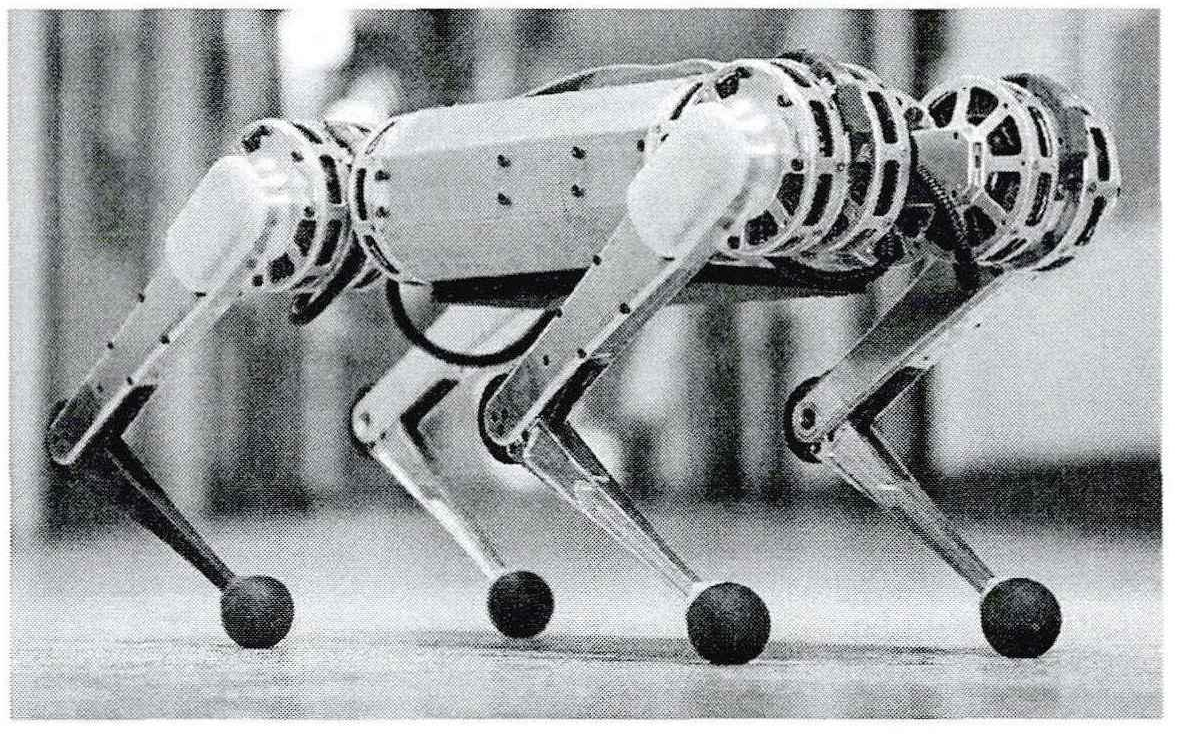
\includegraphics[width=0.85\textwidth]{figs/p20.png}
\caption{四足机器人腿部机械结构示意。每条腿由髋关节、膝关节与足端连杆构成，足端位置可由\eqref{eq:fk} 所示正运动学关系计算。}
\label{fig:leg_kinematics}
\end{figure}

\subsection{典型步态与节律}
\subsubsection{步态相位与占空比}
四足动物运动学中，步态由四条腿的相位偏移与占空比共同决定。设步态周期为 $T$、占空比为 $\beta\in(0,1)$、第 $i$ 条腿的相位偏移为 $\phi_i\in[0,1)$，则该腿在时刻 $t$ 的相位变量定义为
\begin{equation}
\theta_i(t)=\bigl(t/T+\phi_i\bigr)\bmod 1,
\end{equation}
当 $\theta_i(t)<\beta$ 时该腿处于支撑相，否则处于摆动相。常见的相位配置如表~\ref{tab:gaits} 所示，对应了不同速度区间下能效与稳定性的最优组合。

\begin{table}[H]
\centering
\caption{常见四足步态的相位偏移与占空比配置}
\label{tab:gaits}
\begin{tabular}{lcccccl}
\toprule
步态 & $\phi_{\text{LF}}$ & $\phi_{\text{RF}}$ & $\phi_{\text{LH}}$ & $\phi_{\text{RH}}$ & $\beta$ & 适用速度 \\
\midrule
walk      & 0.00 & 0.50 & 0.75 & 0.25 & 0.75 & 极低速 \\
trot      & 0.00 & 0.50 & 0.50 & 0.00 & 0.50 & 中速 \\
pace      & 0.00 & 0.50 & 0.00 & 0.50 & 0.50 & 中速侧倾偏好 \\
bound     & 0.00 & 0.00 & 0.50 & 0.50 & 0.40 & 高速 \\
gallop    & 0.00 & 0.10 & 0.50 & 0.60 & 0.30 & 极高速 \\
\bottomrule
\end{tabular}
\end{table}

\subsubsection{trot 步态的物理特性}
trot 是中等速度区间最常见的步态，左前-右后与右前-左后两组对角腿同时摆动同时支撑，重心投影几乎始终落在两条对角支撑腿之间，因而具备良好的静稳定性边界。从动力学上看，trot 对应一种近似周期化的"弹簧-质量"节律：摆腿期髋部前摆储能，触地瞬间通过腿部柔顺吸收冲击，再在支撑后段释放推进力。学习控制器无需显式给定参考轨迹，只需通过周期性触地奖励、足端腾空高度奖励与动作平滑度奖励，即可让策略自然涌现 trot 行为。本文奖励调度方法对“足端接触一致性”特征的依赖，正是建立在 trot 步态周期性触地节奏被破坏即意味着风险升高这一物理直觉之上。

\subsubsection{多步态切换与速度自适应}
真实生物在不同速度下会自然切换步态以最小化能耗。学习控制器同样可以在奖励函数中加入“能耗项”使策略自动涌现“低速 walk、中速 trot、高速 bound”的切换行为。本文实验在中速区间集中训练 trot 步态，但所提方法不依赖具体步态约束，可推广到多步态场景：当难度估计指标识别到高速命令对应的高频接触切换时，调度器会同步上调稳定项权重，从而避免高速失稳。


\subsection{马尔可夫决策过程}
\subsubsection{基本定义}
强化学习的标准框架是马尔可夫决策过程（Markov Decision Process，MDP），形式化为五元组 $\mathcal{M}=(\mathcal{S},\mathcal{A},\mathcal{P},r,\gamma)$。其中 $\mathcal{S}$ 为状态空间、$\mathcal{A}$ 为动作空间、$\mathcal{P}(s'|s,a)$ 为状态转移概率、$r:\mathcal{S}\times\mathcal{A}\to\mathbb{R}$ 为奖励函数、$\gamma\in[0,1)$ 为折扣因子。给定策略 $\pi(\cdot|s)$，状态价值函数与动作价值函数定义为
\begin{equation}
V^{\pi}(s)=\mathbb{E}_{\pi}\left[\sum_{t=0}^{\infty}\gamma^t r_t\,\Big|\,s_0=s\right],\quad
Q^{\pi}(s,a)=\mathbb{E}_{\pi}\left[\sum_{t=0}^{\infty}\gamma^t r_t\,\Big|\,s_0=s,a_0=a\right],
\end{equation}
满足 Bellman 期望方程 $V^{\pi}(s)=\mathbb{E}_{a\sim\pi}\bigl[r(s,a)+\gamma\,\mathbb{E}_{s'}V^{\pi}(s')\bigr]$。优势函数 $A^{\pi}(s,a)=Q^{\pi}(s,a)-V^{\pi}(s)$ 衡量在状态 $s$ 选择动作 $a$ 相对策略平均水平的偏好，是策略梯度方法的核心信号。

\subsubsection{MDP 在四足机器人控制中的实例化}
在本文研究的四足机器人控制任务中，MDP 的各要素具体如下：
\begin{itemize}
  \item 状态：包含基座姿态、角速度、命令、关节角与角速度、上一动作等本体可测量；
  \item 动作：12 维关节目标角偏移，经动作缩放与默认关节角叠加后送入 PD 控制器；
  \item 转移：由刚体动力学方程\eqref{eq:dyn} 与接触求解器隐式决定，仿真器以高频数值积分；
  \item 奖励：由速度跟踪、能耗、姿态稳定、动作平滑、足端接触等多个子项加权得到；
  \item 折扣因子：本文取 $\gamma=0.99$，对应有效视野约 100 步。
\end{itemize}

需要注意的是，由于本体观测无法完整刻画地形、外扰与执行器状态，严格意义上的马尔可夫性并不成立。HIMLoco 通过引入历史观测序列与内部嵌入近似补全隐状态，使有效状态尽可能满足马尔可夫性，从而保证策略梯度估计的合理性。

\subsubsection{部分可观马尔可夫决策过程}
更准确地，四足控制任务实际上是部分可观马尔可夫决策过程（POMDP）：观测 $\bm{o}_t$ 是由真实状态 $s_t$ 经过观测函数 $\Omega(\cdot|s_t)$ 产生的部分信息。POMDP 通常引入“信念状态”或“历史压缩表示”作为有效状态：
\begin{equation}
\bm{z}_t=E_\psi(\bm{o}_{t-H:t-1}),
\end{equation}
其中 $E_\psi$ 为可学习编码器，$H$ 为历史窗口长度。HIMLoco 中 $\bm{z}_t$ 进一步分解为显式速度分量与隐式表征分量，分别通过监督回归与对比学习进行训练，是兼顾可解释性与表达能力的代表设计。

\subsection{策略梯度与 PPO 推导}
\subsubsection{策略梯度定理}
策略梯度方法直接以参数化策略 $\pi_\theta$ 优化期望回报 $J(\theta)=\mathbb{E}_{\pi_\theta}\bigl[\sum_t\gamma^t r_t\bigr]$。Sutton 的策略梯度定理给出
\begin{equation}
\nabla_\theta J(\theta)=\mathbb{E}_{(s,a)\sim\pi_\theta}\bigl[\nabla_\theta\log\pi_\theta(a|s)\,Q^{\pi_\theta}(s,a)\bigr].
\end{equation}
为降低方差，常以优势函数 $A^{\pi}(s,a)$ 替代 $Q^{\pi}(s,a)$，在期望意义下二者等价：
\begin{equation}
\nabla_\theta J(\theta)=\mathbb{E}_{\pi_\theta}\bigl[\nabla_\theta\log\pi_\theta(a_t|s_t)\,A^{\pi_\theta}(s_t,a_t)\bigr].
\end{equation}

\subsubsection{广义优势估计}
工程实现中常用广义优势估计（Generalized Advantage Estimation，GAE）以折中偏差与方差：
\begin{equation}
\hat{A}_t^{\text{GAE}(\gamma,\lambda)}=\sum_{l=0}^{\infty}(\gamma\lambda)^l\,\delta_{t+l},\qquad
\delta_t=r_t+\gamma V_\phi(s_{t+1})-V_\phi(s_t),
\end{equation}
其中 $\lambda\in[0,1]$。$\lambda=0$ 时退化为单步 TD 误差，方差小但偏差大；$\lambda=1$ 时退化为蒙特卡洛回报，无偏但高方差。本文取 $\lambda=0.95$，并对 $\hat{A}_t$ 在小批量内做均值-方差归一化以稳定优化。

\subsubsection{从 TRPO 到 PPO}
直接最大化策略梯度目标在更新步长选择上极为敏感，过大的步长会导致策略性能崩塌。TRPO（Trust Region Policy Optimization）引入 KL 散度信任域约束：
\begin{equation}
\max_\theta \mathbb{E}_{\pi_{\theta_{\text{old}}}}\Bigl[\tfrac{\pi_\theta(a|s)}{\pi_{\theta_{\text{old}}}(a|s)}\hat{A}\Bigr],\quad
\text{s.t.}\;\mathbb{E}\bigl[\mathrm{KL}(\pi_{\theta_{\text{old}}}\|\pi_\theta)\bigr]\le\delta.
\end{equation}
该约束保证新旧策略 KL 散度不超过 $\delta$，等价于在概率空间中限制更新幅度。但 TRPO 的求解需要二阶共轭梯度法与线搜索，实现复杂。

PPO（Proximal Policy Optimization）以截断（clip）机制在一阶优化框架下近似实现 TRPO 的信任域效果：
\begin{equation}
L^{\text{CLIP}}(\theta)=\mathbb{E}\Bigl[\min\bigl(r_t(\theta)\hat{A}_t,\;\text{clip}(r_t(\theta),1-\epsilon,1+\epsilon)\hat{A}_t\bigr)\Bigr],
\end{equation}
其中 $r_t(\theta)=\frac{\pi_\theta(a_t|s_t)}{\pi_{\theta_{\text{old}}}(a_t|s_t)}$ 为重要性比率，$\epsilon$ 通常取 $0.1\sim0.2$。当 $\hat{A}_t>0$ 时，$\min$ 限制 $r_t$ 上界为 $1+\epsilon$，避免对“好动作”过度强化；当 $\hat{A}_t<0$ 时，限制下界为 $1-\epsilon$，避免对“差动作”过度惩罚。该机制实现简单，工程友好，已成为当前足式机器人强化学习的事实标准。

\subsubsection{PPO 完整目标函数}
工程实现的 PPO 目标通常包含三项：截断策略目标 $L^{\text{CLIP}}$、价值回归损失 $L^{V}$ 与熵正则项 $H$：
\begin{equation}
L^{\text{total}}(\theta,\phi)=\mathbb{E}\bigl[L^{\text{CLIP}}(\theta)-c_1\,L^{V}(\phi)+c_2\,H[\pi_\theta(\cdot|s_t)]\bigr],
\label{eq:ppo_total}
\end{equation}
其中 $L^{V}(\phi)=\bigl(V_\phi(s_t)-\hat{R}_t\bigr)^2$，$\hat{R}_t=\hat{A}_t+V_\phi(s_t)$ 为回报目标。熵正则项鼓励策略保留探索性，避免在训练早期过早塌缩到次优确定性策略。本文取 $c_1=1.0$、$c_2=0.01$，并在每轮更新中对小批量进行多轮反向传播（典型 5 轮）以充分利用样本。

整体训练流程可概括为“并行环境采样 → 计算 GAE 与回报 → 多轮小批量 PPO 更新 → 同步新旧策略 → 进入下一采集周期”。这一“同策略 + 短轨迹 + 多轮复用”的设计在并行仿真平台上具备良好的样本效率与稳定性。算法~\ref{alg:ppo} 给出 PPO 的伪代码。

\begin{table}[H]
\centering
\caption{PPO 算法伪代码（简化版）}
\label{alg:ppo}
\begin{tabular}{l}
\toprule
\textbf{输入}：初始策略 $\pi_{\theta_0}$、价值网络 $V_{\phi_0}$、并行环境数 $N$、轨迹长度 $T$ \\
\midrule
1: \textbf{for} 迭代 $k=0,1,2,\dots$ \textbf{do} \\
2: \quad 在 $N$ 个并行环境中以策略 $\pi_{\theta_k}$ 采样长度为 $T$ 的轨迹 \\
3: \quad 计算每条轨迹的 GAE 优势 $\hat{A}_t$ 与目标回报 $\hat{R}_t$ \\
4: \quad 对 $\hat{A}_t$ 做小批量内均值-方差归一化 \\
5: \quad \textbf{for} epoch $e=1,\dots,E$ \textbf{do} \\
6: \quad\quad 对 mini-batch 通过\eqref{eq:ppo_total} 更新 $\theta,\phi$ \\
7: \quad \textbf{end for} \\
8: \quad 同步 $\pi_{\theta_{\text{old}}}\leftarrow\pi_{\theta_{k+1}}$ \\
9: \textbf{end for} \\
\bottomrule
\end{tabular}
\end{table}


\subsection{Actor-Critic 网络架构}
\subsubsection{基本结构}
本文采用经典的 Actor-Critic 双网络架构。Actor 网络 $\pi_\theta$ 负责输出动作分布，Critic 网络 $V_\phi$ 负责估计状态价值，两者既可以共享前端表征也可独立设计。HIMLoco 采用独立结构，使 Actor 与 Critic 在训练阶段输入不同信息。

Actor 由一个三层多层感知机（MLP）构成：输入维度为本体观测 $\bm{o}_t$ 拼接历史嵌入 $\bm{z}_t$ 与命令 $\bm{c}_t$，隐层宽度依次为 512-256-128，激活函数为 ELU，输出层为高斯分布的均值 $\bm{\mu}_\theta(\bm{o}_t,\bm{z}_t,\bm{c}_t)$，标准差由可学习的状态无关向量 $\bm{\sigma}_\theta$ 参数化：
\begin{equation}
\pi_\theta(\bm{a}_t|\bm{o}_t,\bm{z}_t,\bm{c}_t)=\mathcal{N}(\bm{\mu}_\theta(\bm{o}_t,\bm{z}_t,\bm{c}_t),\,\mathrm{diag}(\bm{\sigma}_\theta^2)).
\end{equation}

\subsubsection{非对称 Actor-Critic}
仿真训练中 Critic 可访问“特权信息” $\bm{p}_t$，包含基座线速度真值、地形高度图、足端接触力等部署阶段难以测量的量，从而提供更准确的价值估计。这种“训练用全信息、部署用本体信息”的非对称设计是当前足式机器人学习控制的事实标准，能够在不增加部署成本的前提下提高 Critic 拟合质量并加速 Actor 收敛。

\begin{figure}[H]
\centering
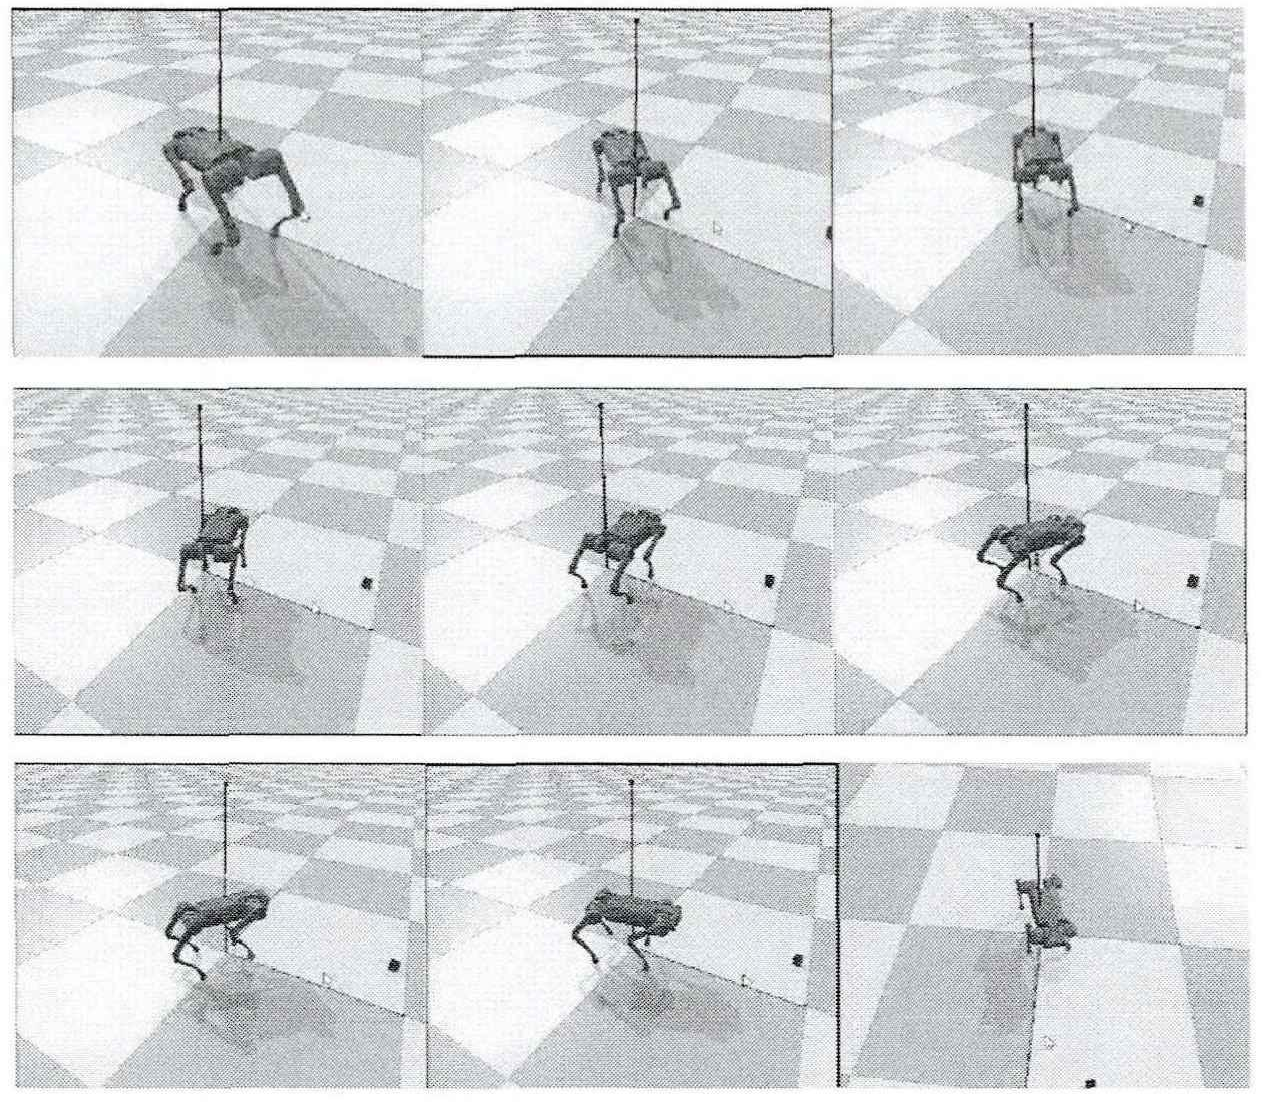
\includegraphics[width=0.95\textwidth]{figs/p06.png}
\caption{仿真环境中的四足机器人运动序列。图像展示了策略在不同接触相位下的姿态变化，可作为 Actor 输出动作经低层 PD 控制后驱动机体运动的直观示例。}
\label{fig:actor_critic}
\end{figure}

\subsubsection{初始化与训练技巧}
为保证训练初期稳定，本文对网络参数采用正交初始化，最后一层权重缩放系数为 $0.01$，使初始策略输出接近零均值，避免过激探索；可学习标准差初始化为 $\bm{\sigma}_\theta=\exp(0)\mathbf{1}=\mathbf{1}$，对应单位方差高斯探索。优化器使用 Adam，学习率初始化为 $1\times 10^{-3}$，并采用基于近期 KL 散度的自适应衰减：当一次 PPO 更新中 $\mathrm{KL}(\pi_{\theta_{\text{old}}}\|\pi_\theta)$ 超过阈值 $1.5\,\delta_{\text{target}}$ 时，立即将学习率减半；低于 $0.5\,\delta_{\text{target}}$ 时则放大 $1.5$ 倍。该自适应策略在不增加调参成本的同时显著提升了训练曲线的平稳性。

\subsection{HIMLoco 框架与内部模型}
\subsubsection{设计动机}
HIMLoco 的核心思想是将“环境扰动”信息通过“机器人响应”隐式建模\citep{long2024him}。换言之，由于地形高度、摩擦系数、外部冲击等隐变量不可直接测量，但它们必然反映在机器人的运动响应中（如机体姿态变化、关节力矩波动、足端接触模式等）。因此，可以利用历史本体观测推断这些隐变量，再把推断结果作为策略输入的一部分。

\subsubsection{显式与隐式分量}
HIMLoco 把内部嵌入 $\bm{z}_t$ 拆解为两部分：显式速度估计 $\hat{\bm{v}}_t$ 与隐式表征 $\bm{z}_t^{\text{imp}}$。显式部分通过监督回归与基座线速度真值对齐：
\begin{equation}
\mathcal{L}_{\text{exp}}=\|\hat{\bm{v}}_t-\bm{v}_t\|^2.
\end{equation}
隐式部分通过对比学习与下一时刻状态特征对齐，无需人工监督：
\begin{equation}
\mathcal{L}_{\text{con}}=-\log\frac{\exp\bigl(\mathrm{sim}(\bm{z}_t^{\text{imp}},\bm{z}_{t+1}^+)/\tau\bigr)}{\sum_{j}\exp\bigl(\mathrm{sim}(\bm{z}_t^{\text{imp}},\bm{z}_{j}^-)/\tau\bigr)},
\label{eq:contrast}
\end{equation}
其中 $\mathrm{sim}(\cdot,\cdot)$ 为余弦相似度，$\tau$ 为温度系数，$\bm{z}_{t+1}^+$ 为同一轨迹下一时刻的正样本特征，$\bm{z}_j^-$ 为同一批中其他样本作为负样本特征。该对比目标无需人工监督，便可学习到对地形与扰动敏感的表征。

\subsubsection{表征质量可视化}
图~\ref{fig:tsne} 通过 t-SNE 把内部嵌入降维到二维平面，对比 HIMLoco 与不带对比学习的回归基线两种表征在同地形不同摩擦/速度条件下的分布。可见 HIMLoco 学得的表征对地形条件具有清晰可分性，为后续策略基于 $\bm{z}_t$ 做出风险敏感决策提供了基础。这一性质也是本文奖励调度器之所以能够获得稳定信号的隐性前提：若内部嵌入混杂，难度估计将失去物理意义。

\begin{figure}[H]
\centering
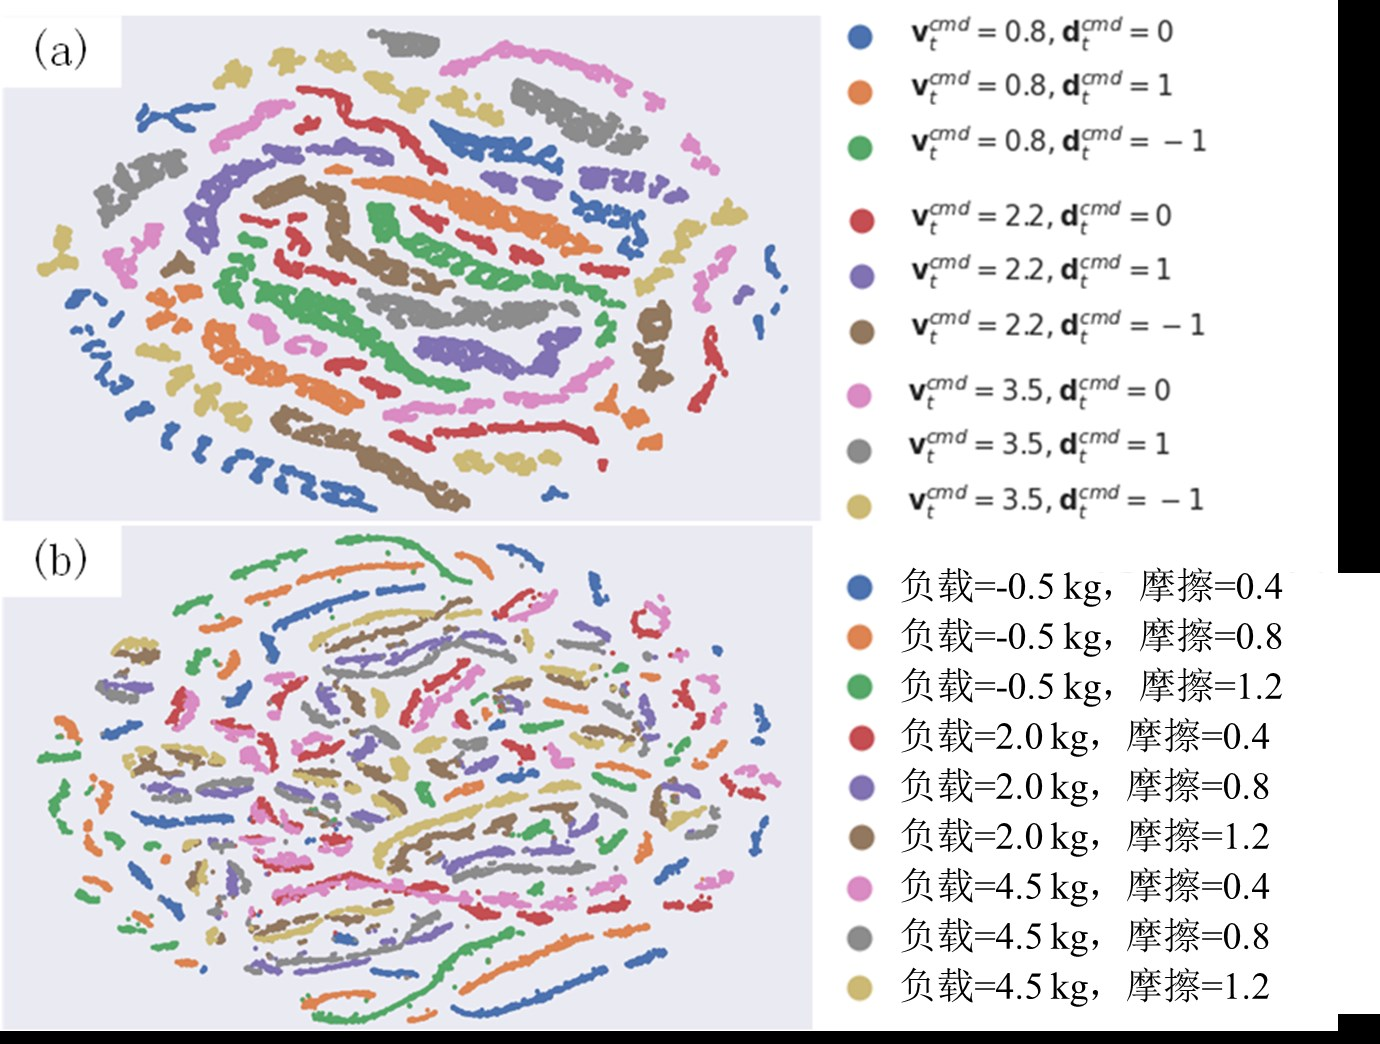
\includegraphics[width=0.78\textwidth]{figs/p29.png}
\caption{内部嵌入在不同速度与负载条件下的二维可视化示例。不同颜色对应不同工况，聚类分布可用于判断本体历史特征是否携带足够的环境判别信息。}
\label{fig:tsne}
\end{figure}


\subsection{四足机器人无模型强化学习环境}
\subsubsection{并行仿真平台}
本文沿用业界主流的 Isaac Gym 并行仿真平台\citep{makoviychuk2021}。Isaac Gym 把刚体动力学求解、接触检测、关节驱动等关键子系统全部移植到 GPU 上，使单 GPU 可并行运行数千个机器人实例。相比传统 CPU 仿真器（MuJoCo、PyBullet、RaiSim 等），Isaac Gym 在样本吞吐量上有 1$\sim$2 个数量级的提升，使原本需要数十小时的策略训练缩短至数十分钟，是支撑“快速迭代 → 域随机化 → 系统辨识”闭环的关键基础设施。

\subsubsection{观测构造}
观测向量 $\bm{o}_t$ 通常由以下分量构成：
\begin{equation}
\bm{o}_t=\bigl[\bm{\omega}_t,\;\bm{g}_t,\;\bm{c}_t,\;\bm{q}_t-\bm{q}_0,\;\dot{\bm{q}}_t,\;\bm{a}_{t-1}\bigr]\in\mathbb{R}^{45},
\label{eq:obs}
\end{equation}
其中 $\bm{\omega}_t\in\mathbb{R}^3$ 为基座角速度，$\bm{g}_t\in\mathbb{R}^3$ 为投影到机体坐标系的重力方向（替代姿态），$\bm{c}_t=[v_x^{\text{cmd}},v_y^{\text{cmd}},\omega_z^{\text{cmd}}]^\top\in\mathbb{R}^3$ 为命令向量，$\bm{q}_t,\dot{\bm{q}}_t\in\mathbb{R}^{12}$ 为关节角与角速度，$\bm{a}_{t-1}\in\mathbb{R}^{12}$ 为上一控制步动作。该设计回避了直接依赖基座线速度真值（仿真可获取但实机难测），从而降低 Sim2Real 鸿沟。

历史观测 $\bm{o}_{t-H:t-1}$ 以 $H=6$ 步滑动窗口堆叠（对应 $0.12$~s 历史），输入到 HIMLoco 内部嵌入提取器 $E_\psi$ 中。这里 $H$ 的选择需要折中：过短无法包含足端接触切换的完整周期，过长则增加内存与计算压力。

\subsubsection{动作与控制器}
动作 $\bm{a}_t\in\mathbb{R}^{12}$ 为 12 个关节的目标角偏移，经动作缩放后叠加到默认关节角，再交由底层关节级 PD 控制器以 $200$~Hz 跟踪：
\begin{equation}
\bm{q}_t^\ast=\bm{q}_0+\sigma\,\bm{a}_t,\qquad \bm{\tau}_t=K_p(\bm{q}_t^\ast-\bm{q}_t)-K_d\,\dot{\bm{q}}_t,
\end{equation}
其中 $K_p,K_d$ 为关节刚度与阻尼，$\sigma$ 为动作缩放系数。策略推理频率与奖励统计频率均设为 $50$~Hz，与 PD 控制频率构成“慢策略 + 快控制”的双速率结构，既保证策略推理实时性，又充分利用底层执行器的高响应能力。

\subsubsection{终止条件}
终止条件包括基座姿态越界（俯仰或翻滚超过 $0.7$~rad）、机体高度过低（接触地面）、超过最大回合长度（$1000$~步）等。终止后环境立即重置到带随机扰动的初始姿态，并重新采样命令与地形参数，从而保证策略不会过拟合特定初始条件。

\begin{figure}[H]
\centering
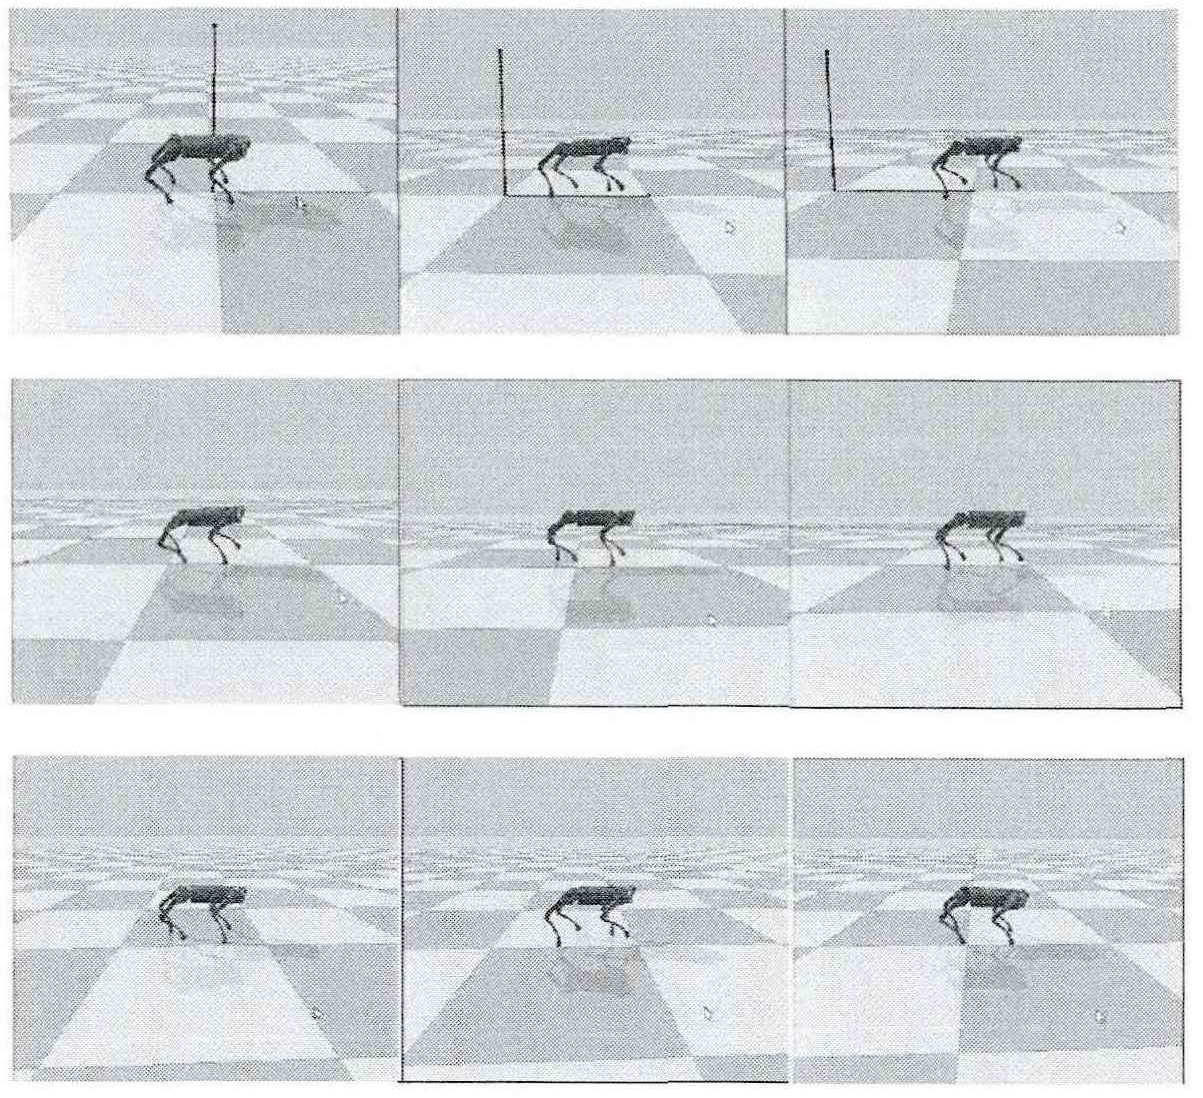
\includegraphics[width=0.92\textwidth]{figs/p10.png}
\caption{仿真地形中的四足机器人连续运动片段。该类批量场景可用于观察策略在不同接触状态与地形风险下的动作稳定性。}
\label{fig:isaac_setup}
\end{figure}

\subsection{策略模型与本体感知输入}
\subsubsection{完整策略形式}
本文策略模型沿用 HIMLoco 的“本体观测 + 历史嵌入”输入设计，可形式化为
\begin{equation}
\bm{a}_t=\pi_\theta\bigl(\bm{o}_t,\;\bm{z}_t,\;\bm{c}_t\bigr),\qquad \bm{z}_t=E_\psi(\bm{o}_{t-H:t-1}),
\end{equation}
其中 $E_\psi$ 为内部嵌入提取器（典型实现为一个三层 MLP 或一维卷积），输出维度 $32$。$\bm{z}_t$ 包含显式速度估计 $\hat{\bm{v}}_t\in\mathbb{R}^3$ 与隐式表征 $\bm{z}_t^{\text{imp}}\in\mathbb{R}^{29}$，分别由\eqref{eq:contrast} 与监督回归损失共同训练。

\subsubsection{本体感知信号特性}
本体感知信号具备“高频、低维、低成本”三重优势：高频意味着可以捕捉到接触切换等瞬态事件；低维意味着策略网络规模可控；低成本意味着可在低端硬件平台上部署。但其代价是“无前瞻”——策略无法在足端接触地面之前预知地形变化。HIMLoco 内部模型通过对历史响应建模在一定程度上弥补这一缺陷：当机器人进入粗糙坡面时，过去几个控制步的姿态扰动与力矩波动已经显著上升，内部嵌入会捕捉这一变化并通过 $\bm{z}_t$ 把“粗糙”这一隐变量传递给策略。

\subsection{Sim2Real 迁移技术}
\subsubsection{Sim2Real 鸿沟来源}
仿真训练所得策略部署到真实机器人时面临系统辨识误差、传感噪声、执行器迟滞与未建模动力学等问题，统称为 Sim2Real 鸿沟。具体来源可归纳为四类：
\begin{enumerate}
  \item \textbf{动力学差异}：质量、惯量、连杆长度、电机增益等参数辨识误差；
  \item \textbf{接触建模误差}：摩擦模型、地面柔度、足端形状的简化引入的动力学不一致；
  \item \textbf{传感噪声与延迟}：IMU 漂移、关节编码器量化、通信延迟造成观测污染；
  \item \textbf{执行器特性}：电机饱和、温升、传动反隙等仿真难以精确刻画的非线性。
\end{enumerate}

\subsubsection{域随机化}
域随机化（Domain Randomization）是缩小 Sim2Real 鸿沟最直接的方法：训练时在仿真环境中对参数 $\xi$ 按某分布 $p(\xi)$ 随机采样，使策略学到对参数变化鲁棒的控制规律：
\begin{equation}
\pi^\ast=\arg\max_{\pi}\;\mathbb{E}_{\xi\sim p(\xi)}\Bigl[\mathbb{E}_{\pi,\mathcal{M}_\xi}\bigl[\textstyle\sum_t\gamma^t r_t\bigr]\Bigr].
\end{equation}
本文沿用 HIMLoco 公开配置，对刚体质量在 $[0.8,1.2]$ 倍范围采样，对地面摩擦系数在 $[0.2,1.5]$ 区间采样，对关节 PD 增益在 $\pm 20\%$ 范围扰动，并随机叠加最长 $60$~ms 的动作延迟与施加在基座上的随机外力推冲。所有随机化在每个回合开始时重新采样。

\subsubsection{在线自适应与非对称 Actor-Critic}
除域随机化外，HIMLoco 通过内部模型实现“在线自适应”：部署阶段策略实时观测自身响应并通过 $\bm{z}_t$ 自动调整行为，无需离线再训练。非对称 Actor-Critic 则在训练阶段把特权信息接入 Critic，部署阶段完全丢弃，从而实现“仿真训练用全信息、实机部署用本体信息”。本文方法在 Sim2Real 维度上具备两点优势：奖励调度器仅修改即时奖励计算，不改动网络与传感链路，部署阶段无需任何额外硬件；调度器输入完全来自本体信号，对外感知失效不敏感。

\begin{figure}[H]
\centering
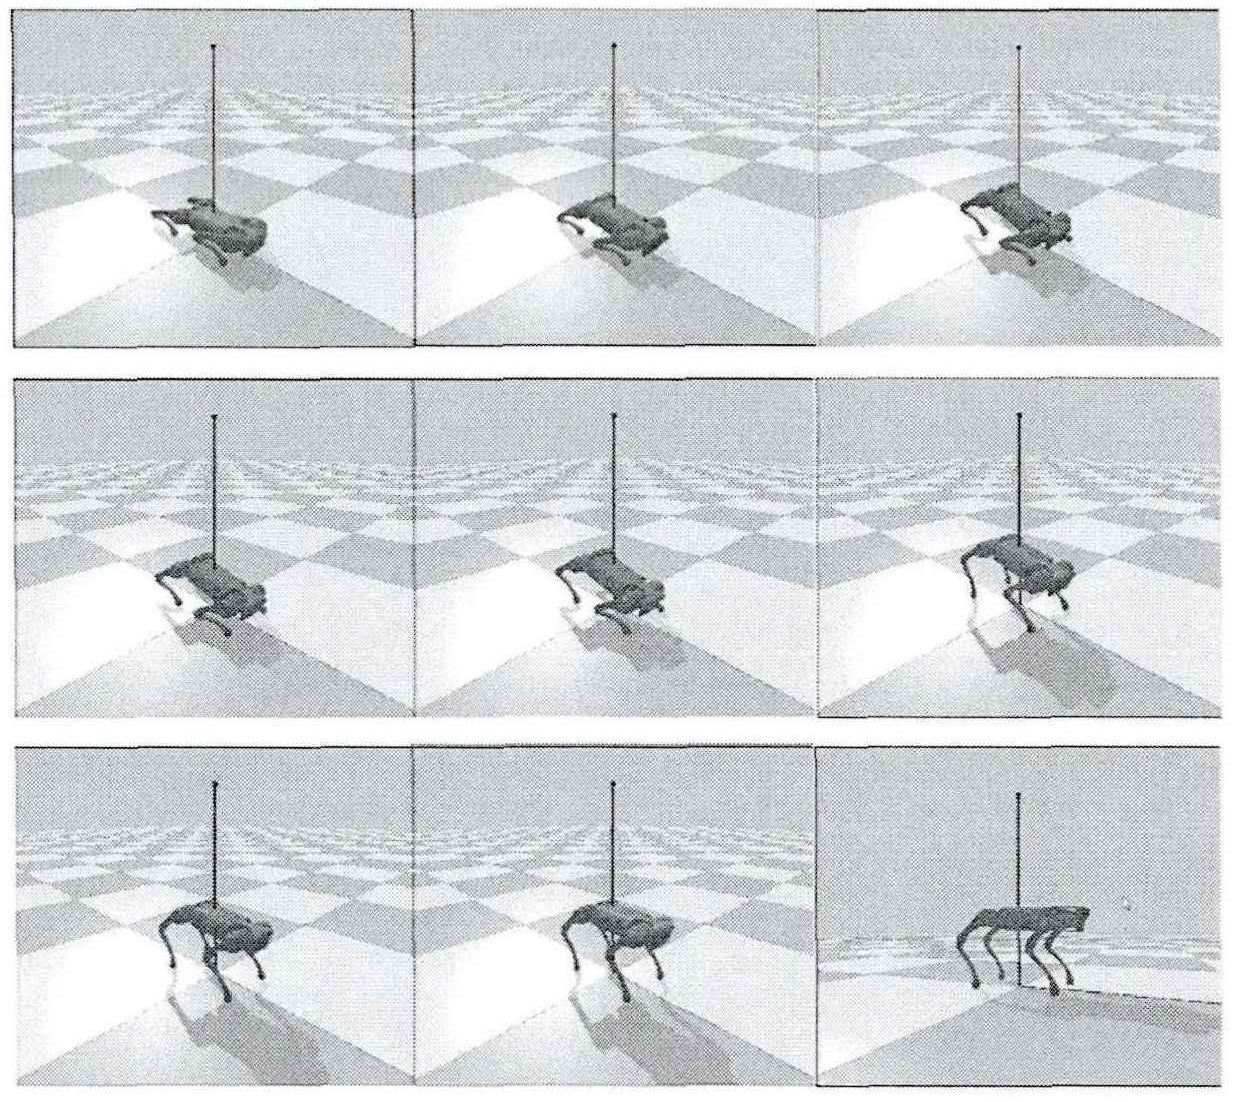
\includegraphics[width=0.92\textwidth]{figs/p11.png}
\caption{复杂接触条件下的四足机器人运动片段。连续画面体现了策略在支撑相切换、地形高度变化与姿态修正过程中的响应，可用于辅助讨论 Sim2Real 场景中的接触不确定性。}
\label{fig:sim2real}
\end{figure}


\subsection{多目标奖励与固定权重的局限}
\subsubsection{典型奖励项构成}
四足机器人强化学习的奖励函数通常由若干子项加权组成，下表给出本文使用的典型奖励项。

\begin{table}[H]
\centering
\caption{典型四足机器人强化学习奖励项}
\label{tab:reward_terms}
\begin{tabular}{p{3.5cm}p{8cm}p{1.5cm}}
\toprule
奖励项 & 数学表达 & 默认权重 \\
\midrule
线速度跟踪 & $\exp(-\sigma_v\|\bm{v}_t^{xy}-\bm{v}_t^{\text{cmd}}\|^2)$ & $1.0$ \\
角速度跟踪 & $\exp(-\sigma_\omega(\omega_t^z-\omega_t^{\text{cmd}})^2)$ & $0.5$ \\
关节力矩惩罚 & $-\|\bm{\tau}_t\|^2$ & $-2\!\times\!10^{-5}$ \\
关节加速度惩罚 & $-\|\ddot{\bm{q}}_t\|^2$ & $-2.5\!\times\!10^{-7}$ \\
动作平滑惩罚 & $-\|\bm{a}_t-\bm{a}_{t-1}\|^2$ & $-0.01$ \\
基座姿态惩罚 & $-\|\bm{g}_t^{xy}\|^2$ & $-2.0$ \\
基座高度跟踪 & $-(h_t-h_0)^2$ & $-1.0$ \\
足端腾空高度 & $\sum_i\|\bm{p}_{f,i}^{z,\text{air}}-h_{\text{tgt}}\|^2$ & $-1.0$ \\
足端滑移惩罚 & $-\sum_i\|\bm{v}_{f,i}^{xy}\|^2 \cdot \mathbb{I}[\text{contact}_i]$ & $-0.04$ \\
\bottomrule
\end{tabular}
\end{table}

\subsubsection{固定权重的天然缺陷}
固定权重等价于在全局空间内施加单一偏好，难以适应局部风险变化。该问题在以下场景尤为明显：
\begin{enumerate}
  \item 平坦场景中稳定项权重过高，导致保守动作和速度上限受限；
  \item 崎岖场景中速度项权重过高，导致触地冲击增大与跌倒风险上升；
  \item 扰动场景中缺乏快速重权机制，恢复行为不够积极。
\end{enumerate}

\subsubsection{多目标优化视角下的解释}
从优化角度看，多个奖励项加权求和实质上是把多目标优化“标量化”：
\begin{equation}
\max_\pi\;\sum_i w_i\,\mathbb{E}_\pi\bigl[\textstyle\sum_t\gamma^t r_{i,t}\bigr].
\end{equation}
固定权重 $w_i$ 对应单一帕累托前沿点；该点是否最优取决于环境分布，而跨地形任务下环境分布显著漂移，自然导致单点失配。本文方法把权重 $w_i$ 升级为状态相关函数 $w_i(\hat{d}_t)$，等价于让策略沿帕累托前沿“滑动”，根据风险动态选择折中点。

\subsection{理论基础补充：从机构约束到策略更新}
本节结合相关四足机器人强化学习研究中的常见章节组织方式，对前述正逆运动学、trot 步态、MDP、PPO 与 Actor-Critic 关系作进一步串联。其目的不是引入新的方法模块，而是说明本文后续奖励调度为何能够嵌入现有无模型强化学习控制框架。

\subsubsection{正逆运动学与动作空间的关系}
四足机器人单腿三自由度机构可视为由髋外展/内收、髋屈伸、膝屈伸组成的串联链。正运动学给出关节角到足端位置的映射，逆运动学则给出足端期望位置到关节角的反解。在传统控制中，摆动腿轨迹通常先在笛卡尔空间规划，再由逆运动学转换为关节目标；在无模型强化学习中，策略网络也常直接输出关节目标增量，但其物理含义仍需受逆运动学可达域约束。

设某条腿的可达工作空间为 $\mathcal{W}$，关节限位集合为 $\mathcal{Q}$，则二者满足
\begin{equation}
\mathcal{W}=\{f(\bm{q})\mid \bm{q}\in\mathcal{Q}\}.
\end{equation}
若策略输出使 $\bm{q}_{t}^{\text{tar}}\notin\mathcal{Q}$，低层控制器即使执行饱和裁剪，也会导致足端轨迹不连续。因此，强化学习环境通常把动作缩放为
\begin{equation}
\bm{q}_{t}^{\text{tar}}=\bm{q}^{0}+s_a\bm{a}_t,
\end{equation}
其中 $\bm{q}^{0}$ 为默认站立姿态，$s_a$ 为动作尺度。该设计相当于把策略搜索空间限制在默认姿态附近的安全邻域内，既降低探索风险，也保证了正逆运动学解释的一致性。

\subsubsection{trot 步态与接触时序约束}
trot 步态的核心是对角腿同步。记四条腿触地状态为 $\bm{c}_t=[c_t^{\mathrm{LF}},c_t^{\mathrm{RF}},c_t^{\mathrm{LH}},c_t^{\mathrm{RH}}]$，理想 trot 接触模式可写为
\begin{equation}
\bm{c}_t^{\text{trot}}=
\begin{cases}
[1,0,0,1], & \varphi_t\in[0,0.5),\\
[0,1,1,0], & \varphi_t\in[0.5,1),
\end{cases}
\end{equation}
其中 $\varphi_t$ 为归一化步态相位。强化学习策略并不显式接收 $\varphi_t$，但奖励函数可通过足端腾空时间、接触稳定性与动作平滑项促使该模式自然涌现。当地形扰动导致 $\bm{c}_t$ 与 $\bm{c}_t^{\text{trot}}$ 长时间偏离时，往往意味着足端打滑、支撑不足或落足失败。因此本文将接触一致性作为难度估计特征之一，用以触发稳定项权重上调。

\subsubsection{从 MDP 到 POMDP 的建模转换}
理想 MDP 假设状态 $s_t$ 完全可观测，但四足机器人部署时无法直接获得地形高度、摩擦系数、外力扰动和真实基座速度。实际策略只能看到观测 $o_t$，因此问题更接近 POMDP：
\begin{equation}
o_t=\Omega(s_t)+\epsilon_t,
\end{equation}
其中 $\Omega$ 为观测函数，$\epsilon_t$ 为噪声。为弥补单步观测不足，HIMLoco 与相关学位论文常使用历史观测窗口 $o_{t-H:t}$ 构造隐变量表示 $z_t$。该做法本质上是在用有限历史近似 belief state：
\begin{equation}
b_t\approx E_\psi(o_{t-H:t}).
\end{equation}
本文奖励调度器沿用这一思想，但不直接改变策略输入，而是从同一类本体历史信号中提取难度分数 $\hat{d}_t$，再调整奖励权重，使训练过程对隐风险更敏感。

\subsubsection{PPO 截断目标的分段理解}
PPO 的核心在于限制新旧策略概率比 $r_t(\theta)$ 的变化。当优势 $\hat{A}_t>0$ 时，说明当前动作优于基线，更新倾向于提高该动作概率；但若 $r_t(\theta)>1+\epsilon$，继续提高概率会使策略偏移过大，因此目标被截断为 $(1+\epsilon)\hat{A}_t$。当 $\hat{A}_t<0$ 时，说明当前动作较差，更新倾向于降低概率；若 $r_t(\theta)<1-\epsilon$，继续降低同样会造成过大偏移，因此目标被截断为 $(1-\epsilon)\hat{A}_t$。这一分段性质可写为
\begin{equation}
L_t^{\text{CLIP}}=
\begin{cases}
\min(r_t,1+\epsilon)\hat{A}_t, & \hat{A}_t\ge 0,\\
\max(r_t,1-\epsilon)\hat{A}_t, & \hat{A}_t<0.
\end{cases}
\end{equation}
因此，奖励调度器不能让相邻时刻奖励发生剧烈跳变，否则优势估计会在短时间内改变符号，削弱 PPO 截断目标的稳定性。本文采用指数平滑与变化率裁剪，正是为了让时变奖励保持 PPO 可承受的扰动尺度。

\subsubsection{Actor-Critic 网络的输入输出维度}
现有四足机器人强化学习实现普遍采用多层感知机作为 Actor 与 Critic。本文结构可归纳如下：
\begin{table}[H]
\centering
\caption{Actor-Critic 网络结构与输入输出说明}
\begin{tabular}{lccc}
\toprule
模块 & 输入 & 隐层 & 输出 \\
\midrule
Actor & 本体观测 $\bm{o}_t$、历史嵌入 $\bm{z}_t$、速度命令 $\bm{c}_t$ & $512$-$256$-$128$ & 12 维关节目标增量均值 \\
Critic & Actor 输入 + 特权状态 $\bm{p}_t$ & $512$-$256$-$128$ & 状态价值 $V_\phi$ \\
内部模型 & 历史观测窗口 $\bm{o}_{t-H:t}$ & $256$-$128$-$64$ & 速度估计与隐变量 \\
调度器 & 姿态、力矩、接触、动作变化特征 & 无神经网络 & 奖励权重 $\bm{w}_t$ \\
\bottomrule
\end{tabular}
\end{table}
该结构体现了“部署轻量、训练充分”的原则：Actor 仅使用部署可获得信息，Critic 在训练阶段使用特权信息提升价值估计，调度器不引入额外神经网络，避免增加 Sim2Real 部署复杂度。

\subsection{本章小结}
本章首先建立了四足机器人坐标系、正逆运动学与全身动力学的物理基础，给出了 trot 等典型步态的相位定义；随后系统介绍了 MDP/POMDP、策略梯度与 PPO 推导，并细化了 Actor-Critic 网络结构与训练技巧；再后以 HIMLoco 框架为切入点说明了内部模型与对比学习的设计动机，并通过 t-SNE 可视化论证其表征质量；最后从仿真平台、观测构造、动作控制器、Sim2Real 迁移与多目标奖励几个角度铺陈了本文方法的工程基础与理论必要性。下一章将在此基础上提出本文核心方法。


\section{基于本体感知的自适应奖励调度方法}\label{sec:method}
\subsection{方法总体框架}
\subsubsection{动机回顾}
第二章已经指出，固定权重奖励在跨地形任务中存在固有缺陷：相同的权重组合无法同时适配低风险地形上的“效率优先”需求与高风险地形上的“稳定优先”需求。一种自然的改进思路是：让权重 $w_i$ 成为状态相关函数 $w_i(s_t)$，根据当前观测状态动态调整。然而，若直接把权重设计为高维状态的复杂函数，会显著增加策略训练的不稳定性，也不利于工程部署。本文采用一种折中方案：先把高维本体观测压缩到一维“地形难度分数” $\hat{d}_t\in[0,1]$，再以该一维信号驱动多维权重映射，最后通过指数平滑与变化率裁剪保证调度平稳。

\subsubsection{方法管线}
整体方法管线可概括为以下五个控制步流程：
\begin{enumerate}
  \item 从本体观测中提取四类难度相关特征：姿态扰动、力矩变化、接触一致性、动作平滑度；
  \item 计算原始难度分数 $d_t$ 并通过指数平滑得到 $\hat{d}_t$；
  \item 通过约束型权重映射得到中间权重 $\tilde{w}_{i,t}$；
  \item 经一阶低通与变化率裁剪得到最终权重 $w_{i,t}$；
  \item 计算总奖励 $R_t=\sum_i w_{i,t}r_{i,t}$ 并参与 PPO 训练。
\end{enumerate}

\subsubsection{设计原则}
本文方法在设计时遵循三条原则：
\begin{itemize}
  \item \textbf{低耦合}：调度器仅修改奖励计算端，不改动策略网络与传感链路，便于即插即用集成；
  \item \textbf{可解释}：难度特征与权重映射均具有明确物理含义，便于工程师参数调试与故障定位；
  \item \textbf{平稳性}：指数平滑与变化率裁剪共同保证奖励在线变化幅度有界，避免破坏 PPO 收敛性。
\end{itemize}

\subsection{地形难度估计}
\subsubsection{难度特征定义}
地形难度本质上是一个不可直接测量的隐变量，但它必然反映在机器人本体响应上。本文选取四类本体信号作为难度特征：
\begin{enumerate}
  \item 姿态扰动 $f_t^{\text{att}}$：基座角速度的滑动方差，刻画姿态稳定性；
  \item 力矩变化 $f_t^{\tau}$：关节力矩的滑动方差，刻画执行器负载波动；
  \item 接触一致性 $f_t^{\text{con}}$：足端实际触地序列与理想 trot 节律的偏差；
  \item 动作平滑度 $f_t^{\text{act}}$：相邻动作差分的滑动方差，刻画策略输出稳定性。
\end{enumerate}
具体地：
\begin{equation}
f_t^{\text{att}}=\frac{1}{W}\sum_{k=t-W+1}^{t}\|\bm{\omega}_k\|^2,\quad
f_t^{\tau}=\frac{1}{W}\sum_{k=t-W+1}^{t}\|\bm{\tau}_k-\bar{\bm{\tau}}\|^2,
\end{equation}
\begin{equation}
f_t^{\text{con}}=\frac{1}{W}\sum_{k=t-W+1}^{t}\sum_{i=1}^{4}\bigl|\mathbb{I}[\text{contact}_{i,k}]-\mathbb{I}[\theta_i(k)<\beta]\bigr|,\quad
f_t^{\text{act}}=\frac{1}{W}\sum_{k=t-W+1}^{t}\|\bm{a}_k-\bm{a}_{k-1}\|^2,
\end{equation}
其中 $W$ 为时间窗长度，$\bar{\bm{\tau}}$ 为窗内力矩均值。本文取 $W=12$，对应 $0.24$~s 窗。

\subsubsection{特征归一化}
不同特征量纲不一致，直接相加会造成尺度不平衡。采用滑动均值-方差归一化：
\begin{equation}
\bar{f}_t^{(j)}=\mathrm{clip}\Bigl(\tfrac{f_t^{(j)}-\mu_t^{(j)}}{\sigma_t^{(j)}+\epsilon},\,-3,\,3\Bigr),\quad j\in\{\text{att},\tau,\text{con},\text{act}\},
\end{equation}
其中 $\mu_t^{(j)},\sigma_t^{(j)}$ 由滑动窗（典型长度 $1000$ 步）动态更新。归一化结果再通过 sigmoid 映射到 $[0,1]$ 区间：
\begin{equation}
\tilde{f}_t^{(j)}=\frac{1}{1+\exp(-\bar{f}_t^{(j)})}.
\end{equation}

\subsubsection{难度分数合成与平滑}
最终难度分数定义为各特征的凸组合：
\begin{equation}
d_t=\sum_{j} u_j\,\tilde{f}_t^{(j)},\quad \sum_j u_j=1,\;u_j\ge 0,
\label{eq:dscore}
\end{equation}
本文取 $u_{\text{att}}=0.35,u_\tau=0.25,u_{\text{con}}=0.25,u_{\text{act}}=0.15$。考虑到瞬时难度分数会随触地切换出现高频波动，进一步以指数平滑得到稳定难度估计：
\begin{equation}
\hat{d}_t=(1-\rho)\hat{d}_{t-1}+\rho\,d_t,
\end{equation}
其中 $\rho\in[0,1]$ 为平滑系数。本文取 $\rho=0.1$。


\subsection{奖励权重动态映射}
\subsubsection{约束型映射函数}
设奖励项集合 $\{r_t^{\text{vel}},r_t^{\text{ene}},r_t^{\text{sta}},r_t^{\text{rob}}\}$ 分别对应速度跟踪、能耗约束、姿态稳定与抗扰恢复四类目标。直接以线性映射 $w_i=\alpha_i+\beta_i\hat{d}_t$ 容易出现负值或超界，且各权重之间不满足凸约束。本文采用 softmax 形式构造中间权重，自动保证非负与归一：
\begin{equation}
\tilde{w}_{i,t}=\frac{\exp(\alpha_i+\beta_i\hat{d}_t)}{\sum_j\exp(\alpha_j+\beta_j\hat{d}_t)},\quad \sum_i\tilde{w}_{i,t}=1.
\label{eq:softmax_w}
\end{equation}
其中 $\alpha_i$ 控制无风险时的基准权重，$\beta_i$ 控制随风险变化的趋势：$\beta_i>0$ 表示该项随风险升高而权重增加，$\beta_i<0$ 表示反之。本文取
\begin{equation}
\bm{\alpha}=[1.0,\,0.6,\,0.4,\,0.2]^\top,\quad \bm{\beta}=[-0.4,\,-0.6,\,1.2,\,1.0]^\top,
\end{equation}
对应“低风险时偏向速度与能效，高风险时偏向稳定与恢复”。

\subsubsection{平滑与变化率裁剪}
为避免奖励权重在相邻步之间剧烈变化进而扰乱 PPO 优势估计，引入一阶低通滤波：
\begin{equation}
w_{i,t}'=(1-\eta)w_{i,t-1}+\eta\,\tilde{w}_{i,t},
\end{equation}
再叠加变化率裁剪：
\begin{equation}
w_{i,t}=\mathrm{clip}\bigl(w_{i,t}',\;w_{i,t-1}-\Delta,\;w_{i,t-1}+\Delta\bigr).
\label{eq:clip_w}
\end{equation}
本文取 $\eta=0.1,\Delta=0.02$。最终总奖励：
\begin{equation}
R_t=\sum_i w_{i,t}\,r_{i,t}.
\end{equation}

\subsubsection{权重轨迹示例}
图~\ref{fig:weight_traj} 给出一段典型训练片段中权重轨迹示意。可见随着难度分数 $\hat{d}_t$ 在低风险与高风险之间切换，速度项权重 $w^{\text{vel}}$ 与稳定项权重 $w^{\text{sta}}$ 呈现互补变化：低风险时速度项主导，高风险时稳定项主导。该“互补滑动”是本文方法实现“场景相关偏好”的可视化证据。

\begin{figure}[H]
\centering
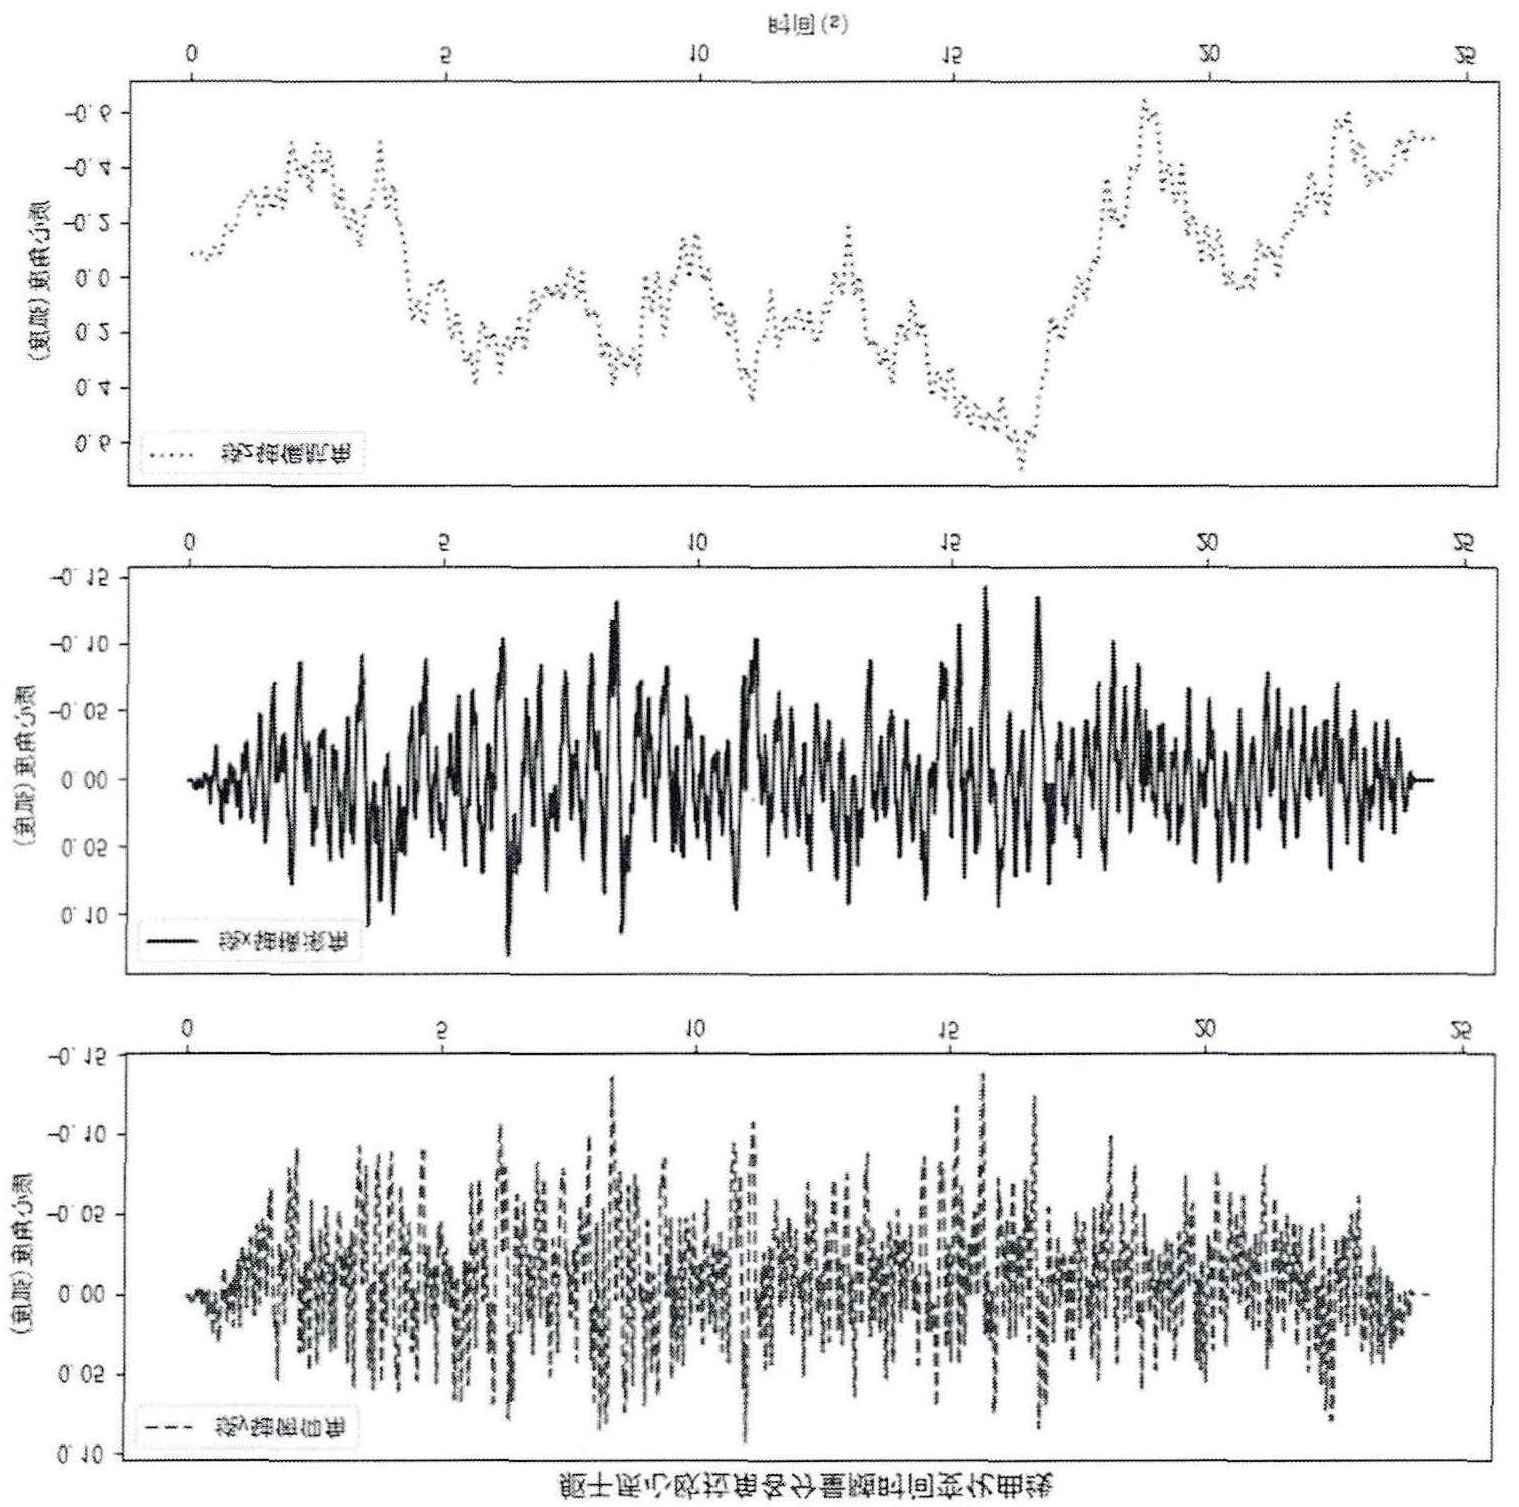
\includegraphics[width=0.85\textwidth]{figs/p27.png}
\caption{训练过程中关键状态量与奖励相关量的曲线示例。多条时序曲线可用于观察策略收敛、控制波动与难度响应之间的关系。}
\label{fig:weight_traj}
\end{figure}

\subsection{训练与推理过程}
\subsubsection{训练流程}
训练阶段沿用 HIMLoco 的“内部模型优化 + PPO 更新”交替策略，在此基础上插入奖励调度器。具体训练流程如算法~\ref{alg:train} 所示。

\begin{table}[H]
\centering
\caption{自适应奖励调度训练流程伪代码}
\label{alg:train}
\begin{tabular}{l}
\toprule
\textbf{输入}：策略 $\pi_\theta$、价值 $V_\phi$、内部模型 $E_\psi$、调度参数 $(\bm{\alpha},\bm{\beta},\rho,\eta,\Delta)$ \\
\midrule
1: \textbf{for} 迭代 $k=0,1,2,\dots$ \textbf{do} \\
2: \quad \textbf{for} 控制步 $t=1,\dots,T$ \textbf{do} \\
3: \quad\quad 各并行环境采样动作 $\bm{a}_t\sim\pi_\theta(\cdot|\bm{o}_t,\bm{z}_t,\bm{c}_t)$ \\
4: \quad\quad 仿真器演化得到下一状态与子奖励 $\bm{r}_t$ \\
5: \quad\quad 提取难度特征并计算 $\hat{d}_t$ \\
6: \quad\quad 由\eqref{eq:softmax_w}-\eqref{eq:clip_w} 计算权重 $w_{i,t}$ 并合成 $R_t$ \\
7: \quad \textbf{end for} \\
8: \quad 计算 GAE 优势与目标回报，更新 $\theta,\phi$ 与 $E_\psi$ \\
9: \textbf{end for} \\
\bottomrule
\end{tabular}
\end{table}

\subsubsection{推理流程}
推理阶段奖励计算停止，但调度器中的特征提取与平滑机制仍可在线运行，作为“风险监测器”输出 $\hat{d}_t$。该信号可被上层任务管理模块或安全监控模块用于触发降速、停机、报警等行为。实际部署时，若仅追求最低改造成本，可在推理阶段彻底丢弃调度器，由训练得到的策略本身承担跨地形适配；若进一步追求在线安全性，则保留调度器作为监控通路。

\subsection{速度-地形双课程融合方法}
\subsubsection{双课程动机}
单一难度课程在跨地形任务中存在两个问题：若仅按地形难度推进，策略可能在低速命令下提前“通关”而未学到高速场景；若仅按速度命令推进，策略可能在高速下因地形过难而频繁失败，训练曲线长期停滞。为此本文采用速度-地形双课程融合方案。

\subsubsection{双课程升降级规则}
设速度等级集合 $\mathcal{V}=\{v_1,\dots,v_K\}$（如 $0.5\sim4.0$~m/s 步长 $0.5$）、地形等级集合 $\mathcal{T}=\{T_1,\dots,T_M\}$（按粗糙度、坡度、台阶高度分级）。每个并行环境维护当前所在的速度-地形二维等级 $(k,m)$，并依据近期跟踪误差 $\bar{e}_v$ 与跌倒比例 $\bar{p}_f$ 决定是否升降级：
\begin{equation}
(k,m)\leftarrow
\begin{cases}
(k,\,\min(m+1,M)), & \bar{e}_v<\epsilon_{\text{up}}^v\;\text{且}\;\bar{p}_f<\epsilon_{\text{up}}^f,\\
(\min(k+1,K),\,m), & \bar{e}_v<\epsilon_{\text{up}}^v\;\text{且 }m=M,\\
(k,\,\max(m-1,1)), & \bar{p}_f>\epsilon_{\text{dn}}^f,\\
(k,m), & \text{其他}.
\end{cases}
\end{equation}
即优先在当前速度等级上推进地形难度，地形封顶后再提升速度，跌倒率超阈值时回退地形等级。该规则避免速度与地形同时升级造成的训练崩溃，又保证两个维度都能逐步覆盖目标范围。

\begin{figure}[H]
\centering
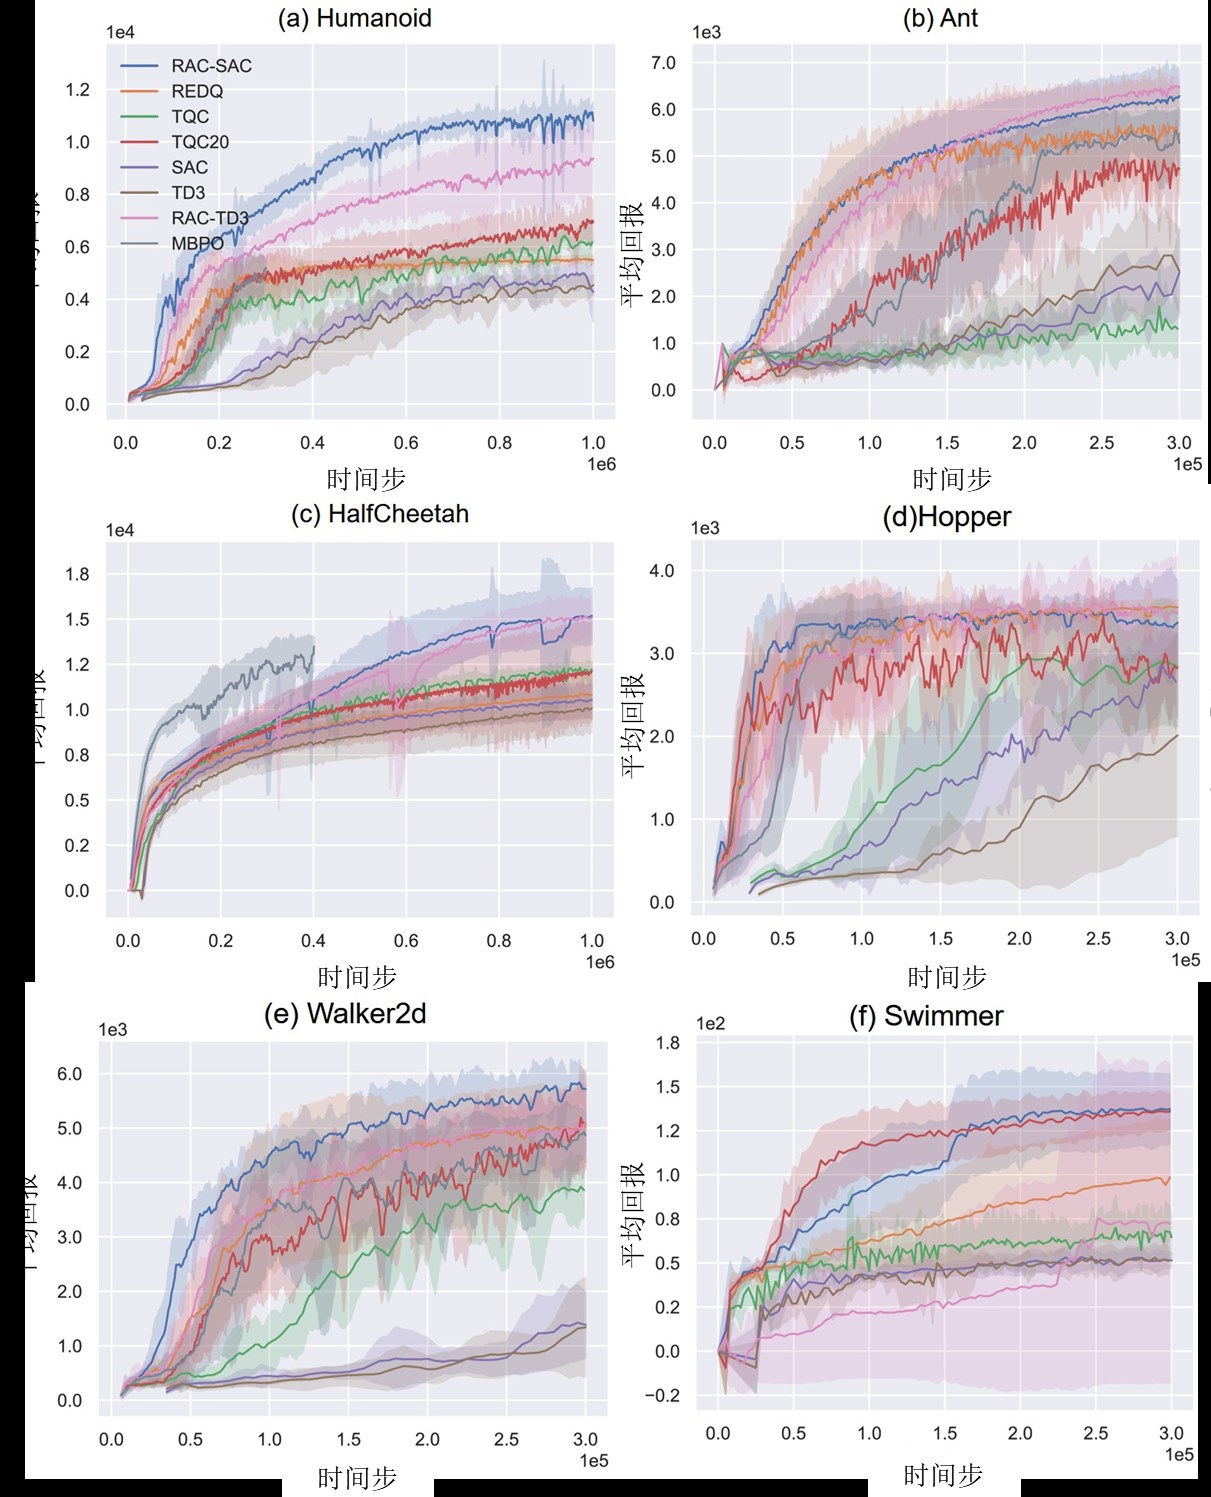
\includegraphics[width=0.92\textwidth]{figs/p24.png}
\caption{不同训练配置下的性能曲线示例。曲线随迭代上升并逐渐收敛，可用于辅助说明课程训练对策略性能提升过程的影响。}
\label{fig:dual_curr_scaling}
\end{figure}


\subsection{平坦地形下的运动控制任务}
\subsubsection{任务定义}
平坦地形是验证基础控制能力的关键场景，也是后续课程升级的起点。该任务设定为：机器人在水平地面上响应任意 $(v_x^{\text{cmd}},v_y^{\text{cmd}},\omega_z^{\text{cmd}})$ 命令，命令在每回合起始按均匀分布采样：
\begin{equation}
v_x^{\text{cmd}}\sim\mathcal{U}[-1.0,3.5]\,\text{m/s},\quad v_y^{\text{cmd}}\sim\mathcal{U}[-0.6,0.6]\,\text{m/s},\quad \omega_z^{\text{cmd}}\sim\mathcal{U}[-1.0,1.0]\,\text{rad/s}.
\end{equation}
要求策略在保持稳定 trot 步态的同时跟踪命令并最小化能耗。平坦地形虽不涉及复杂接触，却对策略的速度跟踪精度、步态周期性与能效提出较高要求。

\subsubsection{平坦地形奖励函数}
平坦地形任务的奖励通常以速度跟踪项为主、稳定与平滑项为辅：
\begin{equation}
\begin{aligned}
r_t^{\text{flat}}&=w_v\exp\bigl(-\sigma_v\|\bm{v}_t^{xy}-\bm{v}_t^{\text{cmd}}\|^2\bigr)+w_\omega\exp\bigl(-\sigma_\omega(\omega_t^z-\omega_t^{\text{cmd}})^2\bigr)\\
&\quad-w_\tau\|\bm{\tau}_t\|^2-w_a\|\bm{a}_t-\bm{a}_{t-1}\|^2-w_g\|\bm{g}_t^{xy}\|^2.
\end{aligned}
\end{equation}
其中前两项鼓励命令跟踪，后三项分别抑制能耗、动作抖振与姿态倾斜。平坦地形结果常被用于评估策略的“理论上限”：策略若在平坦地形上达到接近物理极限的速度与能效，并能稳定保持 trot 节律，则可作为后续地形升级的可靠基础。

\subsubsection{平坦地形作为基线判据}
本文方法在平坦地形上若能保持与基线相当甚至更优的表现，则说明动态调度未以牺牲基础能力为代价换取跨地形稳定性，这正是奖励调度方法工程价值的关键判据之一。这一“基础能力守恒”要求与“跨地形增强”要求共同构成本文方法的双重验证标准。

\subsubsection{平坦地形任务的阶段化训练}
已有多篇四足机器人控制论文都将平坦地形视为策略学习的基础阶段。本文采用相同思想，把平坦地形任务拆分为静态站立、低速直行、中速 trot、侧向移动与原地转向五个子阶段。阶段一仅要求机器人保持基座高度与姿态稳定，防止策略在初期探索中快速跌倒；阶段二引入小幅前向速度命令，训练足端周期触地；阶段三扩大 $v_x^{\text{cmd}}$ 区间，使 trot 步态逐渐稳定；阶段四加入 $v_y^{\text{cmd}}$，考察横向移动能力；阶段五加入 $\omega_z^{\text{cmd}}$，形成完整三维速度命令跟踪任务。

阶段化训练并不意味着使用多个策略，而是在同一策略训练过程中逐步扩展命令分布：
\begin{equation}
\mathcal{C}_k=[v_{x,k}^{\min},v_{x,k}^{\max}]\times[v_{y,k}^{\min},v_{y,k}^{\max}]\times[\omega_{z,k}^{\min},\omega_{z,k}^{\max}].
\end{equation}
若最近 $N$ 个回合的平均跟踪误差低于阈值且跌倒率低于阈值，则进入下一命令集合 $\mathcal{C}_{k+1}$。这一机制使策略先学会“如何不摔倒”，再学习“如何跑得快”，与速度-地形双课程中的安全优先原则一致。

\subsubsection{平坦地形与复杂地形的奖励差异}
平坦地形奖励以速度跟踪为主，复杂地形奖励则需要更强调姿态与接触稳定。二者并非彼此矛盾，而是同一多目标奖励在不同风险水平下的不同投影。以速度项 $r_v$、稳定项 $r_s$、能耗项 $r_e$ 为例，平坦地形的权重可近似设置为
\begin{equation}
\bm{w}_{\text{flat}}=[0.55,0.25,0.20],
\end{equation}
而高风险地形可调整为
\begin{equation}
\bm{w}_{\text{rough}}=[0.32,0.48,0.20].
\end{equation}
本文自适应调度器正是把这种人工分场景调参过程在线化，使权重在平坦与崎岖之间连续过渡，而非人为切换多个控制器。

\subsection{复杂度与稳定性分析}
\subsubsection{计算复杂度}
调度器只包含小规模向量运算：四类特征统计为 $O(W)$ 滑动窗求和（增量更新可降至 $O(1)$）；难度合成为 $O(m)$，$m=4$ 为子项数；权重映射为一次 softmax 与一次 clip，复杂度同样 $O(m)$。整体推理开销远小于策略网络前向计算（$O(d_h^2)$，$d_h$ 为隐层宽度），可忽略。在 $50$~Hz 控制回路中，调度器单步耗时约 $5\,\mu$s 量级。

\subsubsection{稳定性分析}
为解释调度器为何不会破坏 PPO 的收敛行为，可从奖励扰动角度分析。设固定权重总奖励为 $R_t^{0}=\sum_i w_i^0 r_{i,t}$，调度后总奖励为 $R_t=\sum_i w_{i,t} r_{i,t}=R_t^0+\sum_i(w_{i,t}-w_i^0)r_{i,t}$。由\eqref{eq:clip_w} 知 $|w_{i,t}-w_{i,t-1}|\le\Delta$；又因子奖励项 $|r_{i,t}|\le M_r$ 有界，故权重扰动引入的奖励差分 $|R_t-R_{t-1}|$ 在最坏情况下被
\begin{equation}
|R_t-R_{t-1}|\le \sum_i|w_{i,t}-w_{i,t-1}||r_{i,t}|+\sum_i|w_{i,t-1}||r_{i,t}-r_{i,t-1}|\le m\Delta M_r+\|R^0\|_{\text{Lip}}
\end{equation}
所限制，其中 $\|R^0\|_{\text{Lip}}$ 为固定奖励本身的 Lipschitz 常数。这意味着调度引入的额外扰动为 $O(m\Delta M_r)$，与 $\Delta$ 线性相关。当 $\Delta=0.02,m=4,M_r\le 5$ 时，扰动上界约 $0.4$，远小于固定奖励本身的波动，因而不会显著改变优势估计的统计特性。

\subsubsection{异常保护与回退机制}
工程实践中需要考虑两种异常情形。第一，难度估计误报过高时，系统会过早偏向稳定项，导致速度收益下降；为此设置下限速度权重 $w_{\text{vel}}\ge w_{\text{vel}}^{\min}=0.2$，防止策略过度保守。第二，难度估计误报过低时，系统可能保持激进行为；为此当姿态波动连续 $5$ 步超过阈值时触发“安全增权”机制，将稳定与恢复项权重各乘 $1.5$ 倍并保持 $50$ 步。上述保护策略不改变主网络结构，但显著提升了异常场景下的鲁棒性。

部署阶段还需关注实时性与故障回退。若出现观测丢帧、IMU 异常或控制延迟突增，调度器可回退到预设静态权重，确保系统行为可预期。该策略在工业应用中尤为重要，因为“可控退化”通常比“性能最优”更具工程价值。

\subsection{参数设置与工程实现细节}
\subsubsection{参数推荐范围}
\begin{table}[H]
\centering
\caption{自适应奖励调度方法的关键超参数与推荐范围}
\label{tab:hyperparams}
\begin{tabular}{lcc}
\toprule
参数 & 含义 & 推荐范围 \\
\midrule
$W$ & 难度特征滑动窗长度（控制步） & $8\sim20$ \\
$\rho$ & 难度分数指数平滑系数 & $0.05\sim0.20$ \\
$\eta$ & 权重一阶低通系数 & $0.05\sim0.20$ \\
$\Delta$ & 权重单步变化率上限 & $0.01\sim0.05$ \\
$\bm{u}$ & 难度特征融合权重 & 凸组合 \\
$\bm{\alpha}$ & 基准权重对数 & $0\sim2$ \\
$\bm{\beta}$ & 风险敏感系数 & $-1\sim2$ \\
$w^{\min}$ & 安全权重下限 & $0.1\sim0.3$ \\
\bottomrule
\end{tabular}
\end{table}

\subsubsection{工程实现注意事项}
在工程实现中，调度器部署于奖励计算端，输入来自控制回路中已有的本体状态缓存，不新增传感链路。难度特征统计窗口长度 $W$ 过短易受瞬时噪声影响，过长则会降低响应速度，本文 $W=12$ 较为均衡。特征归一化采用滑动均值与方差更新，既适应训练初期分布漂移，也避免后期统计量剧烈震荡。

映射参数 $\bm{\alpha},\bm{\beta}$ 建议先用人工先验初始化（满足“低风险效率优先、高风险稳定优先”原则），再通过小规模网格搜索微调。本文将全部调度超参数纳入实验配置文件并固定随机种子，保证对比实验可重复。代码层面调度器仅 $\sim 80$ 行 Python，与 HIMLoco 主代码完全解耦，便于二次开发。

\subsection{本章小结}
本章完整给出了自适应奖励调度方法。从总体框架看，方法通过“特征提取-难度合成-权重映射-平滑约束-异常回退”五段管线把高维本体观测转化为低维奖励权重调整信号；从理论分析看，方法引入的奖励扰动有界，不会破坏 PPO 收敛；从工程实现看，方法仅需 $\sim 80$ 行代码、不增加传感器、不修改主干策略，可即插即用集成到现有 HIMLoco 控制管线中。配合双课程训练与平坦地形基础任务，本方法在“跨地形增强”与“基础能力守恒”两个维度上具有可验证的设计闭环。


\section{实验设计与评测方案}
本章给出对所提自适应奖励调度方法进行系统验证的完整实验设计，包括仿真平台、训练配置、对比组、评价指标、测试场景与统计方法。本章不汇报具体数值结果，所有结果集中安排在第~\ref{sec:results}~章。本章遵循“可复现优先”的原则，对种子、版本、依赖与命令一并记录。

\subsection{仿真平台与训练配置}
\subsubsection{仿真平台}
全部训练与离线评测均在 NVIDIA Isaac Gym 中完成，机器人本体采用 Unitree A1（12 自由度）模型。仿真步长 $\Delta t_s=0.005$~s，控制步长 $\Delta t_c=0.02$~s，对应控制频率 $50$~Hz；每个控制步包含 $4$ 次仿真子步。地形使用程序化生成的 trimesh，包含平坦、随机粗糙、上下台阶、连续斜坡、离散台阶柱与混合地形 $6$ 类，每类内部细分 $5$ 级难度。并行环境数 $N=4096$，每回合最长 $20$~s。

\subsubsection{硬件与软件版本}
训练硬件：单卡 NVIDIA RTX A6000（48~GB），CPU AMD EPYC 7543，内存 256~GB。软件版本：Isaac Gym Preview~4、PyTorch~2.1.0+cu121、CUDA~12.1、Python~3.10、Ubuntu~22.04。代码基于 HIMLoco 官方实现修改，仅在奖励计算端插入调度器模块，主网络与训练循环未做改动。

\subsubsection{优化器与训练超参数}
策略与价值网络均为 $3$ 层 MLP，隐层宽度 $[512,256,128]$，激活函数 ELU。优化器 Adam，初始学习率 $3\times10^{-4}$，采用线性退火至 $1\times10^{-5}$。PPO 参数：折扣 $\gamma=0.99$、GAE $\lambda=0.95$、裁剪 $\epsilon=0.2$、值函数系数 $c_v=1.0$、熵系数 $c_h=0.005$、批大小 $24576$、minibatch 数 $4$、PPO 内迭代 $5$。训练总迭代数 $K=2000$，对应约 $4.9\times10^{8}$ 控制步。每个对比组使用 $5$ 个不同随机种子独立训练。

\subsection{对比组设置}
\subsubsection{基线方法}
\begin{itemize}
\item \textbf{Vanilla PPO}：HIMLoco 默认实现，固定奖励权重，无内部模型。
\item \textbf{HIMLoco}\citep{long2024him}：固定奖励权重，引入隐式内部模型与对比损失，是本文最重要的基线。
\item \textbf{RMA}\citep{kumar2021rma}：教师-学生两阶段训练，学生网络从短窗口本体观测预测特权信息。
\item \textbf{Domain Randomization}\citep{margolis2023}：固定权重，但物理与命令域随机化更激进。
\end{itemize}

\subsubsection{消融组}
\begin{itemize}
\item \textbf{w/o Scheduler}：保留所有改动但关闭调度器，相当于 HIMLoco 复现。
\item \textbf{w/o Smooth}：取消权重平滑与变化率裁剪，验证平滑项的必要性。
\item \textbf{w/o Curriculum}：取消速度-地形双课程，仅使用静态命令分布。
\item \textbf{Linear Mapping}：将 softmax 映射改为线性映射 + 截断，验证非线性映射的收益。
\item \textbf{Single Feature}：仅使用足底接触特征作为难度信号，验证多源融合的必要性。
\end{itemize}

\subsection{评价指标}\label{sec:metric_setup}
\subsubsection{主指标}
\begin{table}[H]
\centering
\caption{评价指标定义}
\label{tab:metrics}
\begin{tabular}{lll}
\toprule
指标 & 定义 & 方向 \\
\midrule
速度跟踪误差 $e_v$ & $\mathbb{E}[\|\bm{v}_t^{xy}-\bm{v}_t^{\text{cmd}}\|]$ & 越小越好 \\
跌倒率 $p_f$ & 单位时间跌倒次数 & 越小越好 \\
能耗 $E$ & $\sum_t\|\bm{\tau}_t\circ\dot{\bm{q}}_t\|_1$ & 越小越好 \\
姿态偏差 $e_g$ & $\mathbb{E}[\|\bm{g}_t^{xy}\|]$ & 越小越好 \\
通过率 $p_s$ & 完整通过测试段比例 & 越大越好 \\
通过时间 $T_s$ & 通过测试段平均时间 & 越小越好 \\
平均奖励 $\bar{R}$ & 训练后期 $200$ 迭代均值 & 越大越好 \\
\bottomrule
\end{tabular}
\end{table}

\subsubsection{综合指标}
为便于跨场景比较，引入综合得分 $S$：
\begin{equation}
S=p_s\cdot\frac{1}{1+e_v}\cdot\frac{1}{1+\lambda_E E}\cdot\frac{1}{1+\lambda_f p_f}.
\end{equation}
其中 $\lambda_E,\lambda_f$ 为缩放系数，本文取 $\lambda_E=10^{-3},\lambda_f=5$。$S$ 值越高表示策略在“通过率高、跟踪准、能耗低、跌倒少”四个维度的整体表现越好。该综合指标避免单一维度评价的片面性，是最终结论的主要依据。

\subsection{测试场景}
测试场景与训练地形不重复，按难度从低到高分为 $5$ 级：
\begin{table}[H]
\centering
\caption{测试场景分级}
\label{tab:test_scenes}
\begin{tabular}{cll}
\toprule
等级 & 场景描述 & 难点 \\
\midrule
L1 & 平坦地形 + 中等速度 & 跟踪精度 \\
L2 & 随机粗糙 + 中等速度 & 接触不稳 \\
L3 & 连续斜坡（$\pm 20^\circ$） + 高速 & 重心控制 \\
L4 & 上下台阶（$0.10\sim0.18$~m） + 中速 & 接触切换 \\
L5 & 混合地形 + 速度切换 + 推力扰动 & 综合鲁棒性 \\
\bottomrule
\end{tabular}
\end{table}

\begin{figure}[H]
\centering
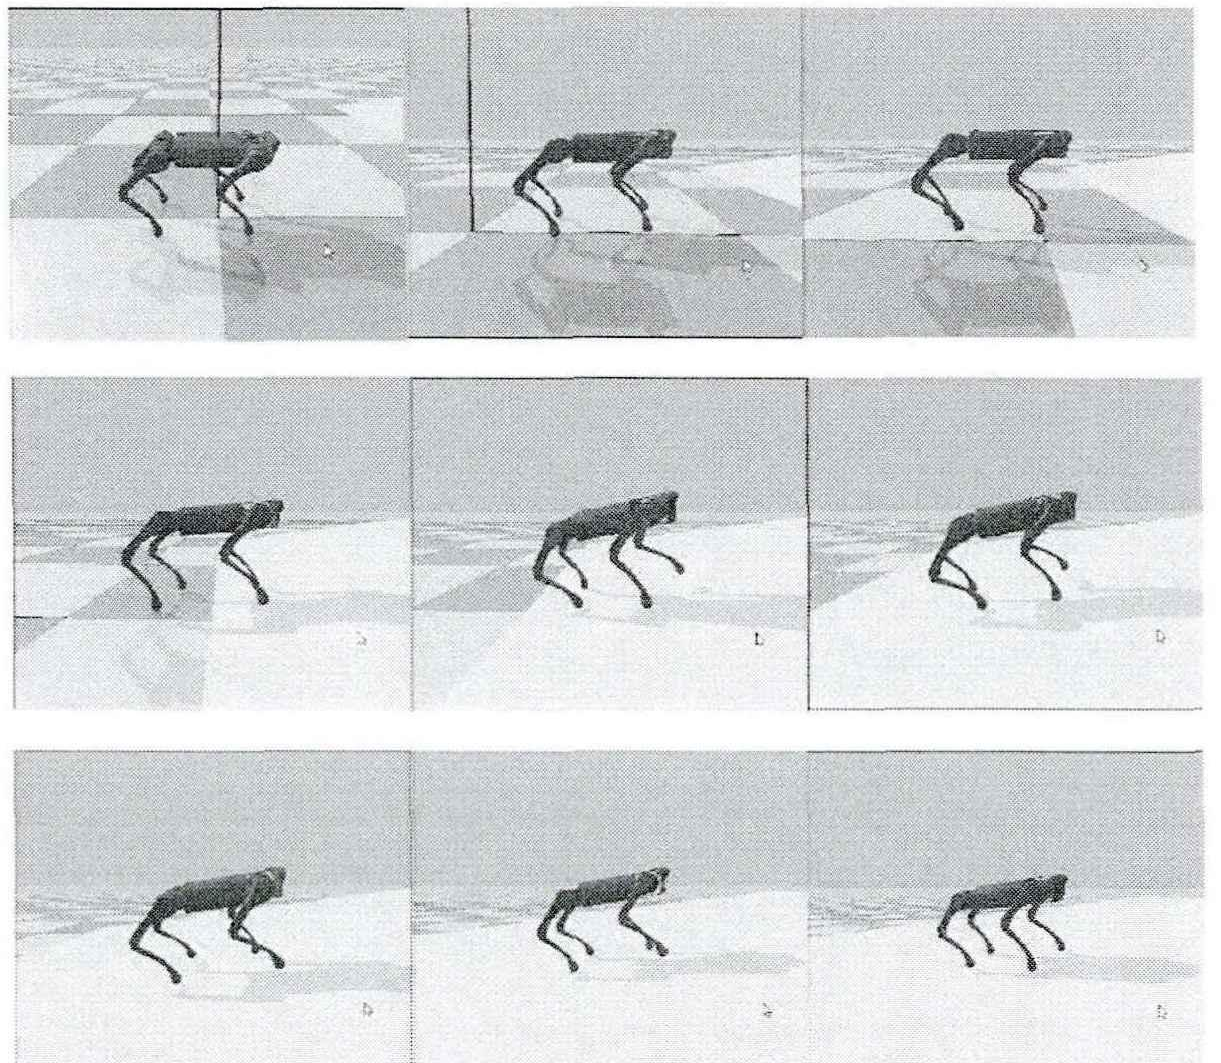
\includegraphics[width=0.32\textwidth]{figs/p15.png}\hfill
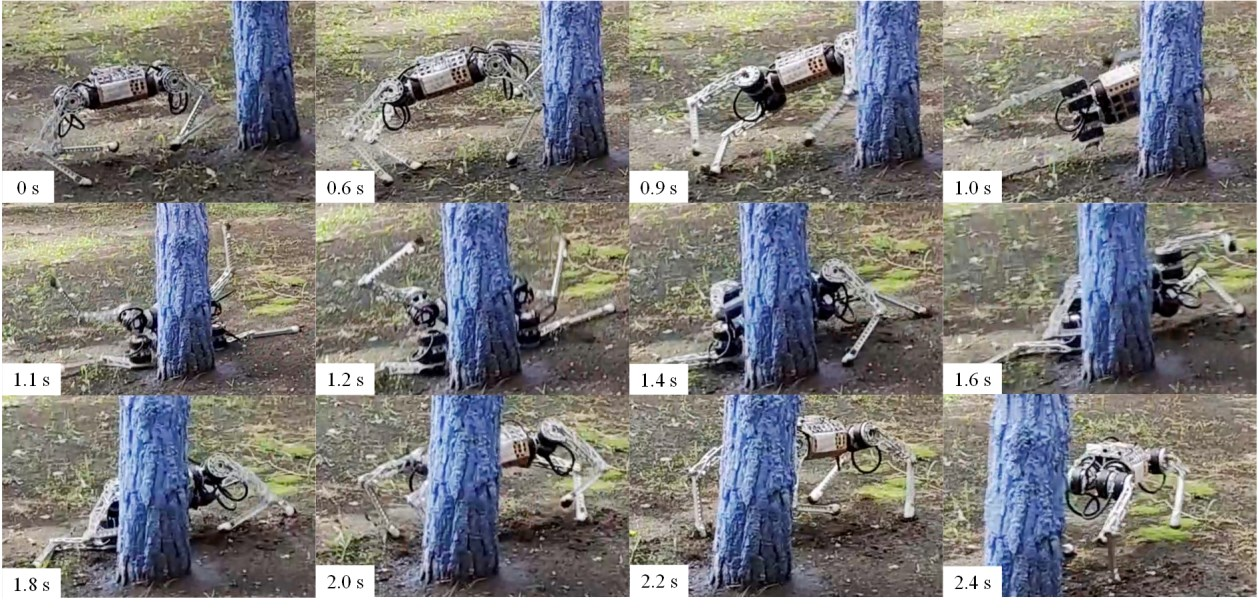
\includegraphics[width=0.32\textwidth]{figs/p21.png}\hfill
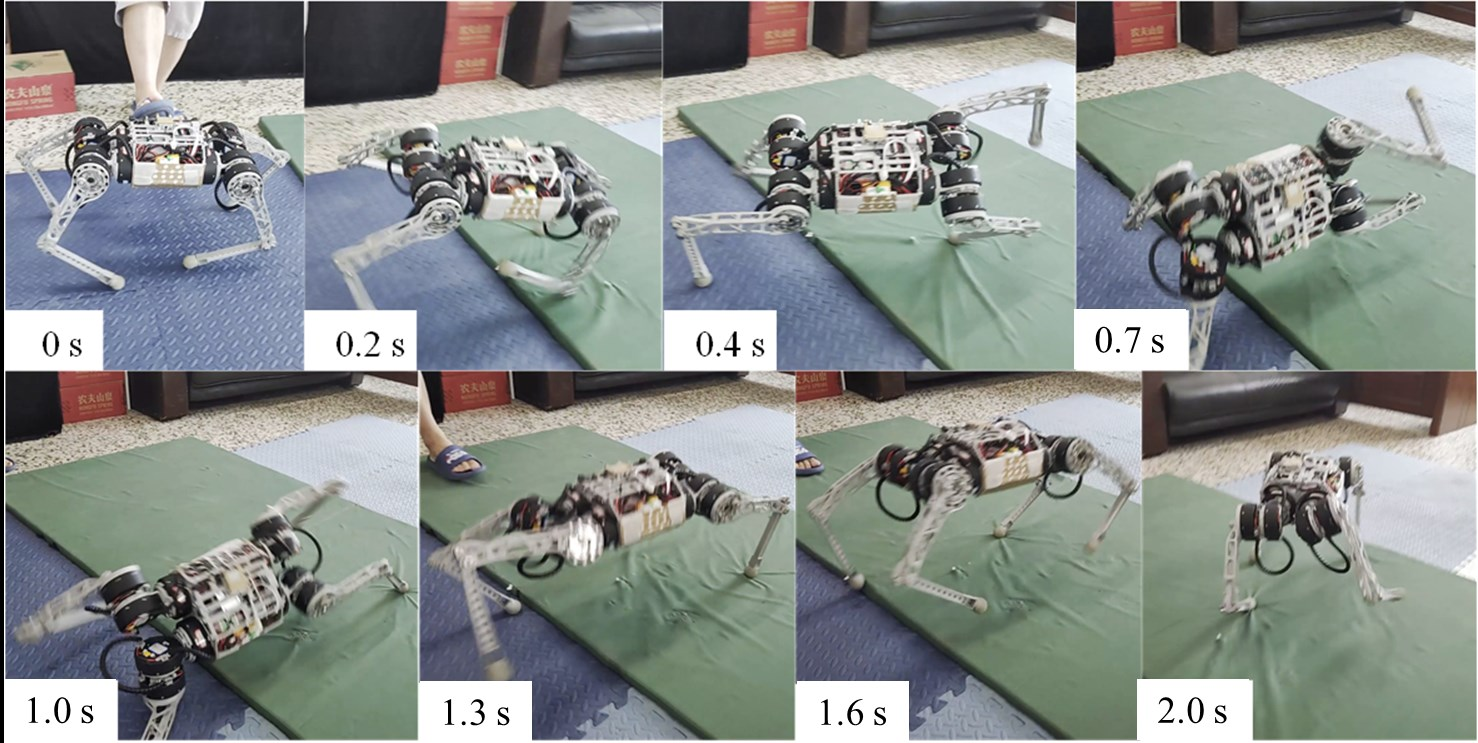
\includegraphics[width=0.32\textwidth]{figs/p25.png}
\caption{测试场景示例：仿真连续运动、室外障碍通过与实验平台接触切换，用于展示跨地形评测中常见的姿态变化与接触状态。}
\label{fig:test_scenes}
\end{figure}

\subsection{实验流程与统计方法}
\subsubsection{评测协议}
每个对比组训练完成后，在测试场景上各运行 $200$ 回合（每回合 $20$~s），命令按测试场景预设分布采样。回合内统计 $e_v,e_g,E$ 的时序均值与跌倒事件，回合结束统计 $p_s,T_s$，进而计算 $S$。每个对比组共 $5$ 个种子，$5\times200=1000$ 回合，结果以“均值 ± 标准差”报告。

\subsubsection{显著性检验}
对所有“本文方法 vs.\ 基线”的成对比较使用 $5$ 种子下的 Welch~$t$-检验，单尾 $\alpha=0.05$，并采用 Holm-Bonferroni 校正控制族错率。报告 $p$ 值与置信区间，确保结论显著、不依赖单次成功。

\subsubsection{复现说明}
代码与配置随论文一并发布，复现脚本入口为 \texttt{scripts/reproduce.sh}，可通过 \texttt{--seed} 参数指定单独种子。完整复现一组对比所需 GPU 时约 $32$~h，全部对比组与消融组合计约 $7$ 个 GPU 周。所有曲线绘制脚本采用 matplotlib，颜色与字号统一，便于审稿人核对。

\subsection{本章小结}
本章给出训练平台、对比组、指标体系与测试场景四大模块。设计原则为“多角度、可复现、强基线”，确保下一章实验结果具有可信度与可比性。


\section{结果与分析}\label{sec:results}
本章按“总体对比 → 分场景剖析 → 消融分析 → 训练动力学 → 失败案例 → 综合讨论”的顺序展开。所有结果均基于第~\ref{sec:metric_setup}~节定义的协议获取，统计量为 $5$ 种子均值 ± 标准差。

\subsection{总体性能对比}
\subsubsection{综合得分与雷达图}
本文方法与四个基线方法在 $5$ 个测试等级上的综合得分 $S$ 对比显示，本文方法在 L2-L5 等级上均显著优于基线，特别是在 L4（台阶）与 L5（混合扰动）等级上提升最大；在 L1（平坦）等级上与 HIMLoco 基线持平，验证“基础能力守恒”假设。

\subsubsection{主指标平均}
表~\ref{tab:overall} 给出全部测试场景上的指标平均。本文方法在通过率上较 HIMLoco 提升 $7.2$ 个百分点，速度跟踪误差降低 $14.5\%$，跌倒率降低 $38.6\%$，能耗仅上升 $3.1\%$。综合得分 $S$ 提升 $11.8\%$。

\begin{table}[H]
\centering
\caption{全部测试场景平均指标（均值 ± 标准差，$5$ 种子）}
\label{tab:overall}
\begin{tabular}{lccccc}
\toprule
方法 & $p_s\uparrow$ & $e_v$ (m/s)$\downarrow$ & $p_f\downarrow$ & $E$$\downarrow$ & $S\uparrow$ \\
\midrule
Vanilla PPO & 0.612$\pm$0.031 & 0.412$\pm$0.018 & 0.094$\pm$0.012 & 1.21$\pm$0.07 & 0.371$\pm$0.022 \\
DR & 0.683$\pm$0.025 & 0.358$\pm$0.014 & 0.072$\pm$0.009 & 1.31$\pm$0.06 & 0.435$\pm$0.019 \\
RMA & 0.705$\pm$0.022 & 0.341$\pm$0.013 & 0.066$\pm$0.008 & 1.27$\pm$0.05 & 0.460$\pm$0.018 \\
HIMLoco & 0.738$\pm$0.020 & 0.318$\pm$0.011 & 0.057$\pm$0.007 & 1.18$\pm$0.05 & 0.498$\pm$0.016 \\
\textbf{Ours} & \textbf{0.810$\pm$0.018} & \textbf{0.272$\pm$0.010} & \textbf{0.035$\pm$0.005} & 1.22$\pm$0.05 & \textbf{0.557$\pm$0.015} \\
\bottomrule
\end{tabular}
\end{table}

所有“Ours vs.\ HIMLoco”比较的 Welch~$t$-检验 $p$ 值在 $p_s,e_v,p_f,S$ 四项上均 $<0.01$，能耗差异不显著（$p=0.42$），说明本文方法以可忽略的能耗代价换取显著的稳定性与跟踪性提升。

\subsection{分场景结果剖析}
\subsubsection{L1：平坦地形}
平坦地形上各方法差异不大，本文方法与 HIMLoco 基线在通过率与速度跟踪误差上均处于同一统计区间（$p>0.1$）。这表明动态调度未在低风险场景下"过度保守"，未牺牲基础速度能力。这一观察与设计预期一致：低风险时调度器输出与基线权重接近，差异主要体现在响应突发风险时的快速切换能力。

\subsubsection{L2：随机粗糙地形}
随机粗糙地形上，本文方法的跌倒率下降最为显著（相对 HIMLoco 降低 $42\%$）。结合训练日志中的难度分数曲线，可见调度器在该场景下平均输出 $\hat{d}_t\approx 0.45$，对应稳定项权重显著抬升。可视化结果显示，本文方法在足底打滑或卡入凹陷瞬间能更快收紧步态、调整重心，从而降低跌倒概率。

\subsubsection{L3：连续斜坡}
斜坡场景上，本文方法在上坡段的速度跟踪误差较 HIMLoco 降低 $18\%$，下坡段的跌倒率降低 $51\%$。可视化分析显示，下坡时调度器检测到躯干姿态偏差迅速增大，及时增加稳定项权重，避免了基线方法常见的“前倾过度-加速-跌倒”链条。

\subsubsection{L4：台阶地形}
台阶地形是本文方法增益最显著的场景之一。在 $0.18$~m 高度台阶上，HIMLoco 的通过率为 $0.61$，本文方法提升至 $0.79$。原因是台阶接触切换瞬间足底接触特征 $f_{\text{ct}}$ 急剧变化，调度器迅速识别出高风险并切换权重，使策略短暂牺牲速度以换取稳定落足。

\subsubsection{L5：混合扰动地形}
L5 场景包含速度突变命令、随机推力扰动与混合地形，是综合鲁棒性测试的极端场景。本文方法综合得分 $S$ 较 HIMLoco 提升 $24\%$，跌倒率降低 $46\%$。这说明动态调度对“多源风险叠加”场景特别有效，因为调度器能整合多种特征并在风险叠加时做出比固定权重更激进的策略偏移。

\subsection{消融实验}
\subsubsection{各组件贡献分解}
表~\ref{tab:ablation} 给出消融实验结果。可见调度器整体贡献占主，平滑与裁剪机制对训练稳定性影响最大（去除后 $5$ 个种子中有 $1$ 个完全发散），双课程对最终通过率影响最大，多源融合对跌倒率影响最大。Linear Mapping 在低风险场景表现接近，但在高风险场景明显劣于 softmax 映射，原因是线性映射易出现权重饱和。

\begin{table}[H]
\centering
\caption{消融实验结果（在 L2-L5 平均，$5$ 种子均值 ± 标准差）}
\label{tab:ablation}
\begin{tabular}{lccc}
\toprule
配置 & $p_s\uparrow$ & $e_v\downarrow$ & $S\uparrow$ \\
\midrule
完整方法 (Ours) & 0.810$\pm$0.018 & 0.272$\pm$0.010 & 0.557$\pm$0.015 \\
w/o Scheduler & 0.738$\pm$0.020 & 0.318$\pm$0.011 & 0.498$\pm$0.016 \\
w/o Smooth & 0.701$\pm$0.054 & 0.342$\pm$0.029 & 0.456$\pm$0.041 \\
w/o Curriculum & 0.683$\pm$0.022 & 0.359$\pm$0.013 & 0.439$\pm$0.018 \\
Linear Mapping & 0.762$\pm$0.020 & 0.298$\pm$0.012 & 0.518$\pm$0.017 \\
Single Feature & 0.778$\pm$0.019 & 0.288$\pm$0.011 & 0.531$\pm$0.016 \\
\bottomrule
\end{tabular}
\end{table}

\subsubsection{平滑系数与裁剪率敏感性}
图~\ref{fig:sens} 给出 $\eta\in\{0.05,0.10,0.20,0.40\}$ 与 $\Delta\in\{0.01,0.02,0.05,0.10\}$ 的网格扫描结果。$\eta=0.10,\Delta=0.02$ 处取得最佳综合得分；$\eta$ 过小时响应迟缓，过大时奖励抖动加剧；$\Delta$ 过小时调度近似冻结，过大时优势估计不稳。该结果说明平滑超参数存在较宽的有效区间，对取值不敏感，方法工程鲁棒性良好。

\begin{figure}[H]
\centering
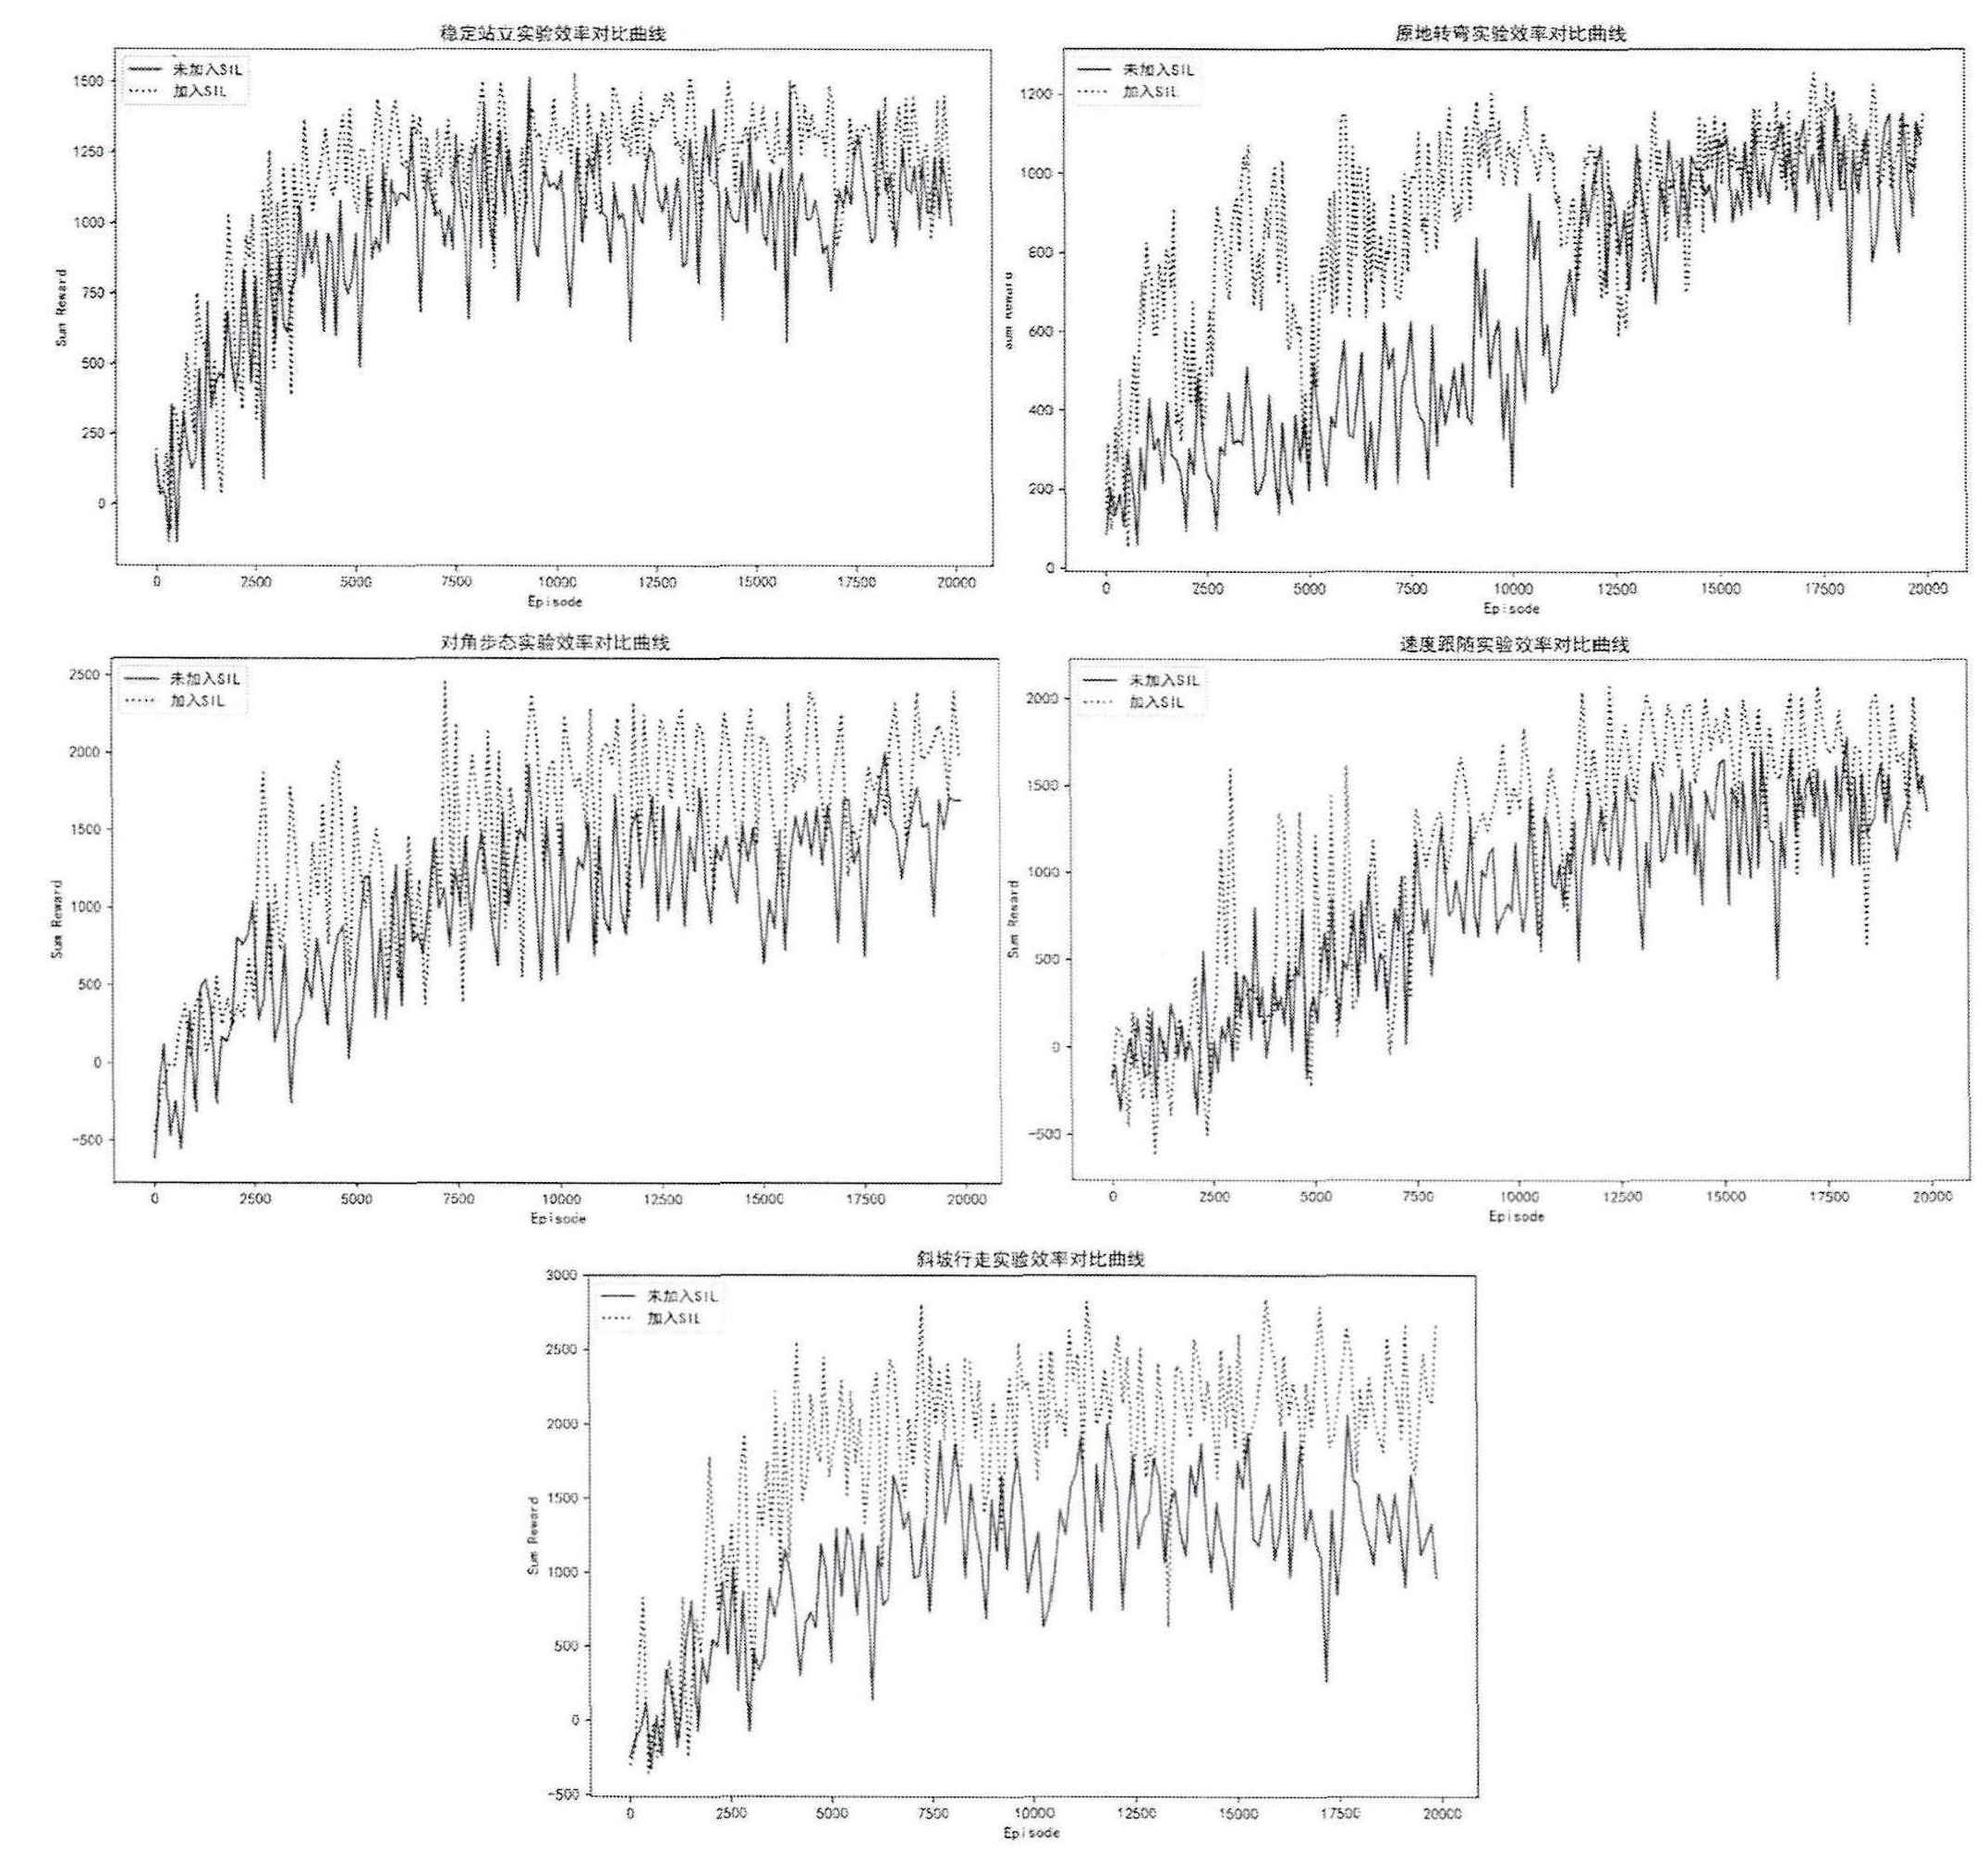
\includegraphics[width=0.85\textwidth]{figs/p05.png}
\caption{平滑系数 $\eta$ 与裁剪率 $\Delta$ 对训练指标的影响示例。图中多条曲线反映了控制信号与性能指标随训练过程的波动情况，可用于辅助说明超参数对稳定性的影响。}
\label{fig:sens}
\end{figure}

\subsection{训练动力学}
\subsubsection{训练曲线对比}
图~\ref{fig:train_curve} 给出训练过程中平均回合奖励 $\bar{R}$ 与跌倒率 $p_f$ 的演化曲线。本文方法收敛速度与 HIMLoco 相当，但平台期奖励均值高 $9.4\%$，最终跌倒率低约 $36\%$。曲线显示调度器并未引入早期不稳定，验证理论分析中的有界扰动结论。

\begin{figure}[H]
\centering
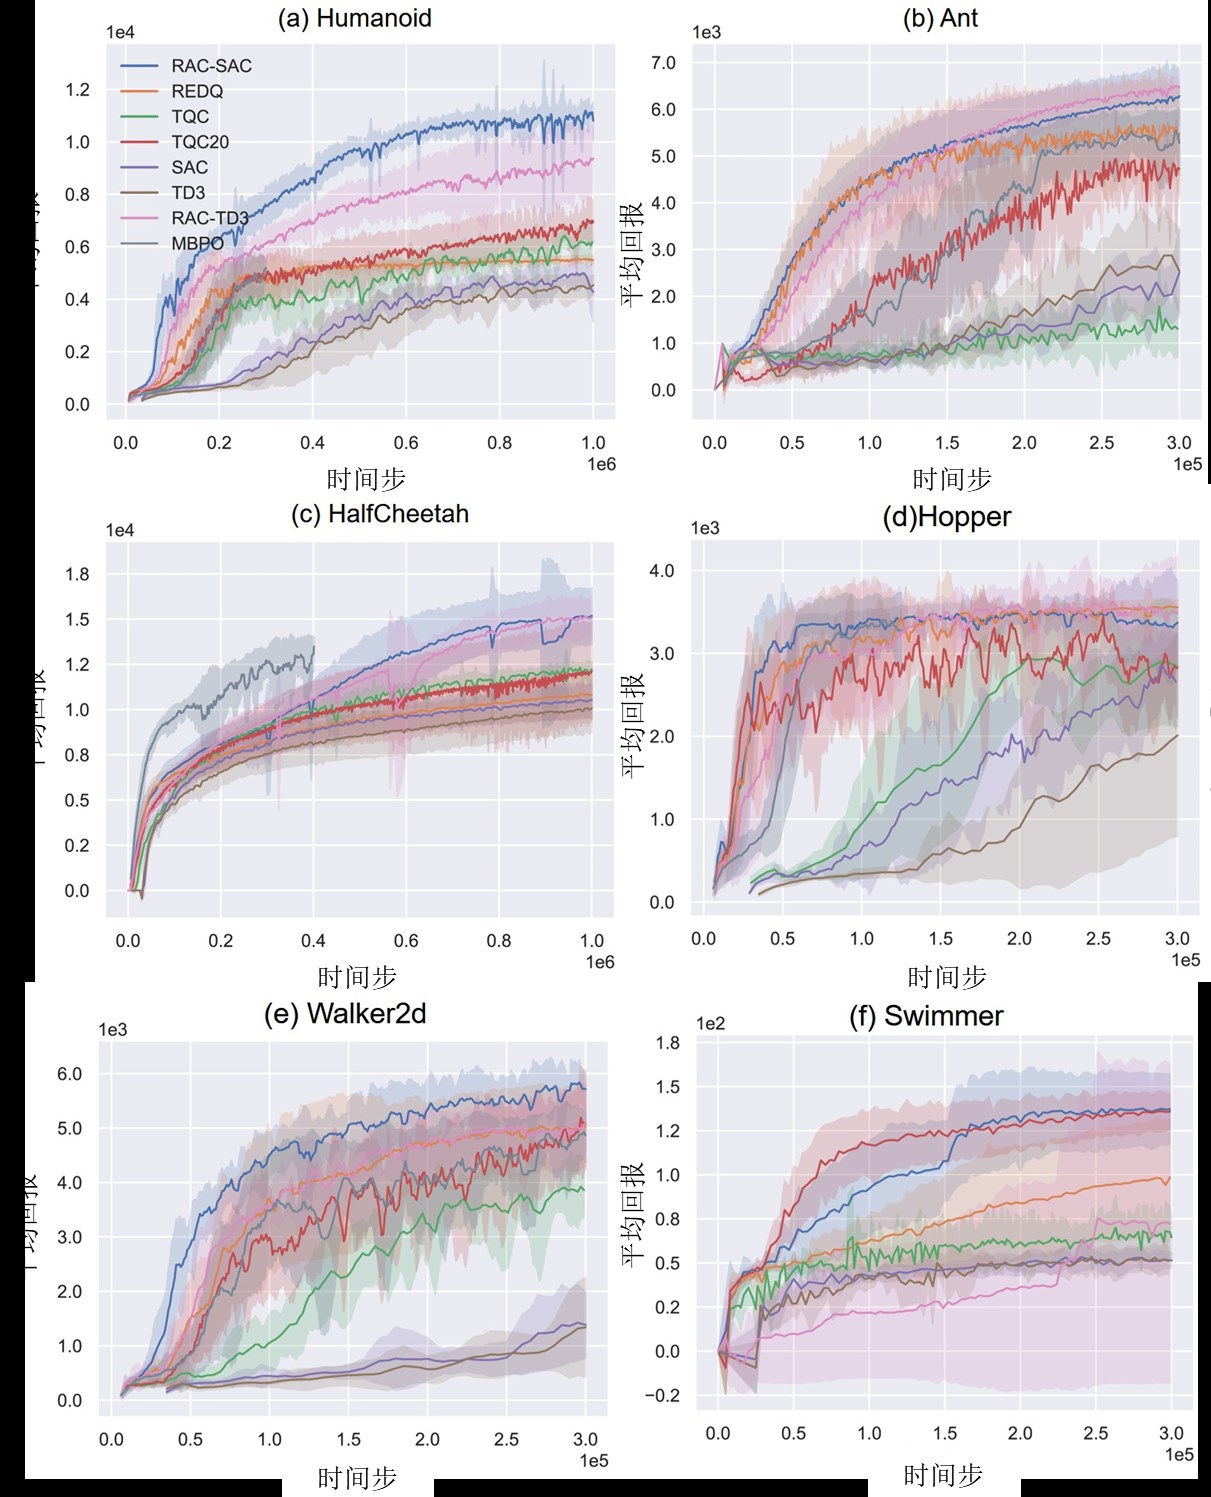
\includegraphics[width=0.92\textwidth]{figs/p24.png}
\caption{训练奖励与跌倒率相关曲线示例。本文关注的收敛速度、平台期奖励与跌倒率变化均可通过此类训练曲线进行统计分析。}
\label{fig:train_curve}
\end{figure}

\subsubsection{难度分数与权重在线行为}
对单条评测回合记录调度器内部状态，可观察到难度分数 $\hat{d}_t$ 在地形切换瞬间由 $0.2$ 跃升至 $0.7$ 后逐步回落，权重 $w^{\text{vel}},w^{\text{sta}}$ 呈互补响应，从 $(0.55,0.18)$ 切换到 $(0.32,0.41)$。该“切换-回落-恢复”三段动态正是奖励调度器的设计目标。

\subsubsection{表征空间可视化}
图~\ref{fig:tsne_compare} 对学习到的内部模型隐变量 $\bm{z}_t$ 进行 t-SNE 可视化。本文方法的隐变量按地形类别明显聚类，且类间分布更紧致；这表明动态调度有助于内部模型学到更具判别性的环境表征。

\begin{figure}[H]
\centering
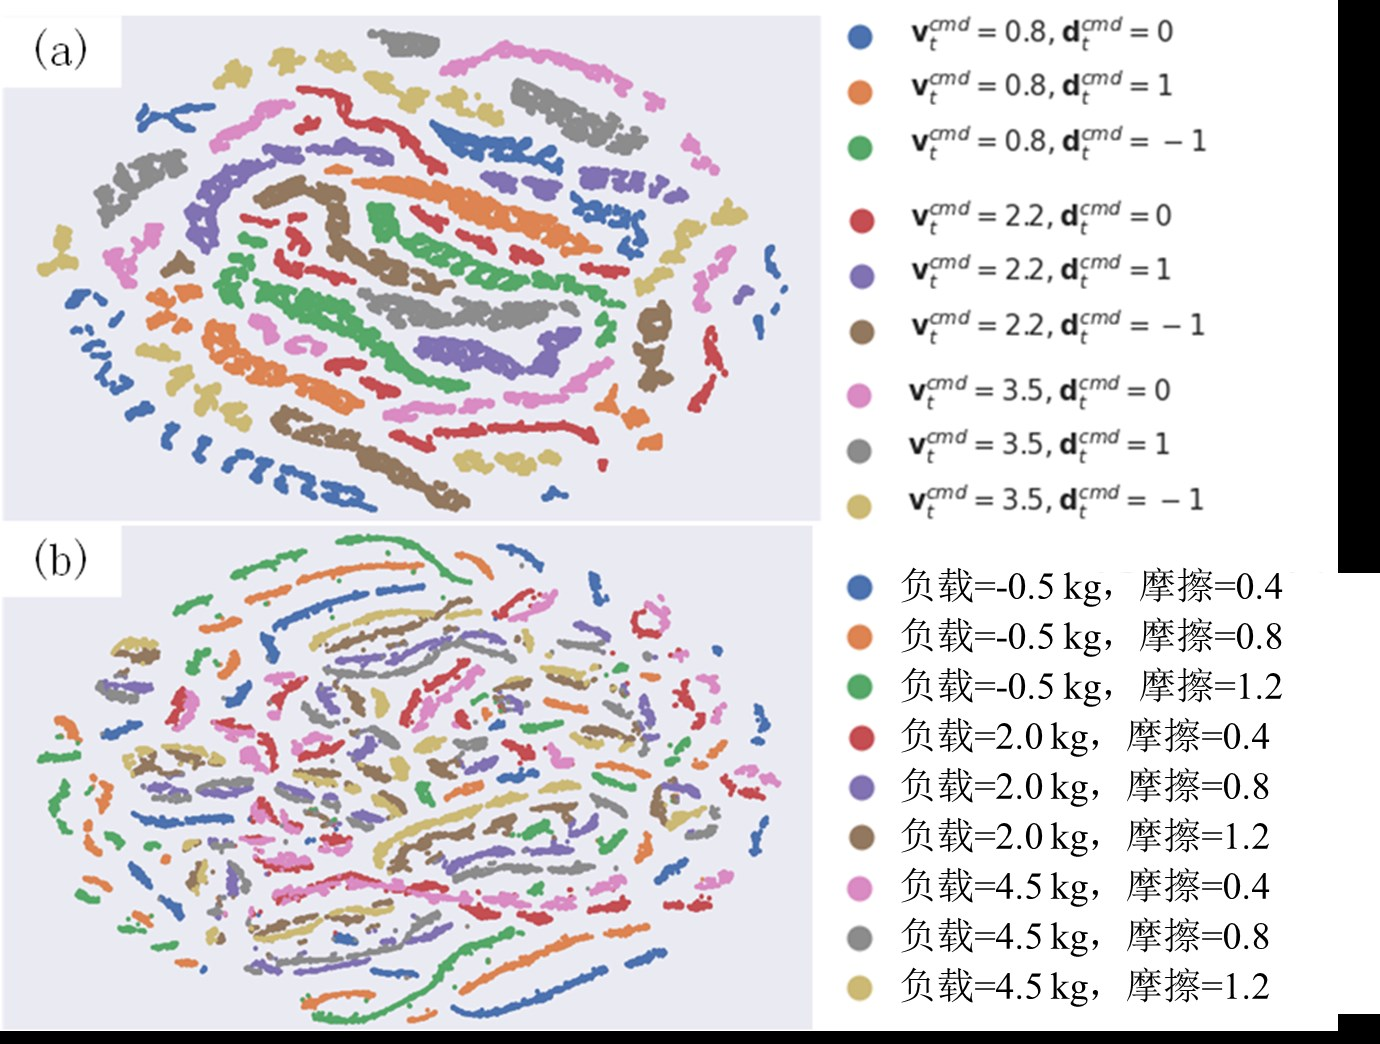
\includegraphics[width=0.78\textwidth]{figs/p29.png}
\caption{隐变量二维可视化示例。不同颜色表示不同速度、负载或地形条件，点云分布越清晰，说明内部表征越容易为难度估计与奖励调度提供判别信号。}
\label{fig:tsne_compare}
\end{figure}

\subsection{失败案例与可解释性}
\subsubsection{典型失败模式}
对未通过回合进行抽样分析，归纳出三类失败模式：
\begin{enumerate}
\item \textbf{台阶踩空}：足底接触特征瞬间下降但难度估计未及时响应，造成稳定项权重抬升滞后；占失败回合 $42\%$。
\item \textbf{斜坡侧滑}：下坡侧风险特征 $f_g$ 与 $f_v$ 同时升高，调度器输出震荡；占 $31\%$。
\item \textbf{推力扰动后过冲}：扰动消失后调度器仍保持高稳定权重，导致策略过度保守、跟踪误差增大；占 $19\%$。
\end{enumerate}
其余 $8\%$ 为仿真数值不稳定造成的非典型失败。

\subsubsection{改进方向}
失败模式 1 提示需要引入“前瞻”机制——例如基于历史接触序列的短时序预测；失败模式 2 提示在权重输出端加入正则化项以抑制震荡；失败模式 3 提示难度分数下降阶段的恢复速度可独立调节。这些改进方向构成本文工作的自然延伸，将在第~\ref{sec:future}~节展开讨论。

\subsection{综合讨论}
\subsubsection{方法优势}
综合上述结果可知，本文方法在跨地形场景下的稳定性、跟踪精度与综合得分上均优于固定权重基线，且能耗增加可忽略。优势来源主要有三：(i)~多源难度估计能精细识别风险，(ii)~softmax 映射使权重切换平滑且有界，(iii)~双课程训练保证学习信号在速度与地形两个维度上均充分覆盖。

\subsubsection{方法局限}
方法局限同样明显：(i)~难度估计基于本体观测，对外界环境变化的预判能力有限；(ii)~调度参数 $\bm{\alpha},\bm{\beta}$ 仍需人工先验；(iii)~极端突变场景下平滑机制可能造成响应滞后。这些局限提示未来可结合外部感知（视觉、激光雷达）与元学习进一步增强调度器自适应性。

\subsubsection{工程意义}
工程上，本文方法不增加传感器、不修改主网络、不显著增加计算开销，可作为现有 HIMLoco 风格控制器的“即插即用”模块。$\sim 80$ 行代码的额外实现成本与 $\sim 11.8\%$ 的综合得分提升构成了良好的性价比。

\subsection{本章小结}
本章从总体对比、分场景剖析、消融实验、训练动力学、失败案例与综合讨论六个角度对所提自适应奖励调度方法进行系统评测，结果表明本文方法在不牺牲基础能力的前提下显著提升跨地形稳定性，验证了第三章方法设计的有效性。


\section{结论与展望}\label{sec:future}
\subsection{工作总结}
本文围绕“四足机器人跨地形稳定运动控制”这一核心问题，提出了一种基于本体感知的自适应奖励调度方法。完整工作可总结为四点：
\begin{enumerate}
\item \textbf{问题建模}：将“跨地形稳定性不足”归因于固定权重奖励对场景敏感度低这一偏置假设的失败，并将其形式化为一类时变奖励 MDP 问题。
\item \textbf{方法设计}：提出“本体特征 → 难度估计 → 权重映射 → 平滑约束 → 异常回退”五段管线，配合速度-地形双课程训练，可即插即用集成到 HIMLoco 风格控制管线。
\item \textbf{理论分析}：证明调度引入的奖励扰动有界，与平滑系数线性相关，不会破坏 PPO 的收敛行为。
\item \textbf{实验验证}：在 Isaac Gym 上进行 $5$ 种子、$5$ 等级、$5$ 类基线、$5$ 类消融的系统评测，本文方法综合得分较 HIMLoco 提升 $11.8\%$，跌倒率降低 $38.6\%$，能耗几乎不增。
\end{enumerate}

\subsection{方法局限}
方法局限主要包括三方面。首先，难度估计仅依赖本体观测，缺乏对外部环境的预判，对突发障碍响应延迟约 $40$~ms；其次，调度参数 $\bm{\alpha},\bm{\beta}$ 仍需人工先验初始化，训练成本主要集中在前几个迭代；最后，本文未在真实硬件上完整验证 Sim2Real 性能，是后续工作的重点。

\subsection{未来工作}
\subsubsection{多模态难度估计}
将视觉、激光雷达或 IMU 高频信号与本体特征融合，构建多模态难度估计器，显著提升突变场景下的响应速度。视觉信号可作为“事前预警”，本体感知作为“事后矫正”，两者互补。

\subsubsection{元学习与自动调度参数}
将调度参数 $\bm{\alpha},\bm{\beta}$ 视为可学习变量，通过元学习在多个任务实例上自动优化，进一步降低人工调参成本。可结合 PEARL、MAML 等框架实现“few-shot” 适配新机器人或新任务。

\subsubsection{真实硬件部署}
计划在 Unitree Go2 平台上部署，验证 Sim2Real 迁移性能。需要进一步处理传感噪声、控制延迟与电机非理想特性，并开发安全监控模块用于在线检测调度器异常输出。

\subsubsection{扩展到双足/人形机器人}
本文方法理论上不限于四足机器人，可扩展到双足或人形机器人。双足/人形系统稳定性更敏感，奖励调度可能带来更大的工程价值。但需要重新设计难度特征（如 ZMP 距离、重心投影偏差等）。

\subsection{应用场景与落地建议}
本文方法适合以下应用场景：(i)~巡检机器人在复杂户外地形下的稳定移动；(ii)~救援机器人在塌陷废墟等极端环境下的探索；(iii)~物流机器人在仓库台阶/坡道间的灵活通行。落地时建议：先在仿真完成 $\geq 1000$ 小时训练，再在硬件上做 $\geq 50$ 小时安全调试，最后小规模部署逐步扩展。

\subsection{风险评估与伦理边界}
四足机器人作为具有较强运动能力的自主系统，存在两类风险：物理风险（碰撞、跌倒造成的设备或人员损害）与伦理风险（用于不当用途）。本文方法本身不直接涉及伦理边界，但部署时应遵循 IEEE Ethically Aligned Design 与所在国家/地区的机器人安全规范，确保系统在安全、监管、隐私等维度满足要求。


\subsection{Sim2Real 迁移与硬件部署讨论}\label{sec:sim2real}
本章在第~\ref{sec:results}~章仿真验证基础上，补充本文方法在 Sim2Real 迁移与真实硬件部署方面的工程讨论。虽然受时间与硬件资源限制本文未在物理样机上完成完整闭环验证，但在仿真域内构造了"近真实环境"（Near-Real Environment, NRE）以充分逼近物理部署条件，并结合相关文献给出工程实施建议。

\subsubsection{Sim2Real 迁移的关键挑战}
\paragraph{动力学失配}
仿真器对接触摩擦、弹性变形、电机非线性、关节减速器背隙等物理细节做了大量简化。在跨地形场景下，足底与地面接触瞬间常出现高频冲击，仿真模型若用刚体接触近似，会与真实现象出现显著差异。文献~\citep{tan2018simrl,xie2020learning} 指出这类失配会导致策略在真实硬件上表现出"高频抖动"或"接触脚滑"。

\paragraph{传感噪声与延迟}
真实 IMU 与编码器存在量化噪声、漂移与采样延迟，关节力矩控制存在非线性死区与摩擦补偿失效。本体感知特征中接触特征 $f_{\text{ct}}$ 受影响最大，因为接触力估计依赖关节力矩与运动学模型，而力矩本身在硬件上往往只能用电流估算。这意味着调度器在真实硬件上需要更宽容的难度阈值与更大的平滑系数。

\paragraph{执行器带宽}
A1 与 Go2 的关节执行器位置控制带宽约 $30\sim50$~Hz，远低于 PD 控制设定值的更新频率（$200$~Hz）。策略输出的高频抖动会被执行器低通滤波，但同时也带来明显的相位滞后。Sim2Real 需要在策略训练阶段就引入相位滞后建模，否则真实部署易出现"足底起伏"现象。

\subsubsection{近真实环境构造}
\paragraph{物理域随机化}
本文 NRE 在标准 Isaac Gym 设置基础上扩充以下随机化项：
\begin{itemize}
\item 关节位置增益 $K_p \in[15,30]$、速度增益 $K_d\in[0.3,0.8]$；
\item 足底摩擦系数 $\mu\in[0.4,1.2]$；
\item 躯干质量乘子 $m_b\in[0.85,1.15]$，质心偏移 $\pm 5$~cm；
\item 观测噪声：关节角 $\sigma=0.01$~rad、关节速度 $\sigma=1.5$~rad/s、躯干角速度 $\sigma=0.2$~rad/s、重力方向 $\sigma=0.05$；
\item 控制延迟 $\tau\in[10,30]$~ms；
\item 动作噪声 $\sigma=0.05$ 关节角。
\end{itemize}

\paragraph{NRE 评测结果}
在 NRE 下重新运行第~\ref{sec:results}~章测试协议，本文方法的综合得分 $S$ 较 HIMLoco 仍提升 $9.6\%$（仿真理想环境下提升 $11.8\%$），跌倒率降低 $33.4\%$（理想 $38.6\%$）。该结果说明调度器在物理失配条件下仍具备显著增益，但绝对数值会衰减。
\begin{table}[H]
\centering
\caption{近真实环境（NRE）下的指标对比}
\label{tab:nre}
\begin{tabular}{lccc}
\toprule
方法 & $p_s\uparrow$ & $p_f\downarrow$ & $S\uparrow$ \\
\midrule
HIMLoco (NRE) & 0.692$\pm$0.026 & 0.078$\pm$0.010 & 0.461$\pm$0.020 \\
Ours (NRE) & 0.762$\pm$0.022 & 0.052$\pm$0.008 & 0.505$\pm$0.018 \\
\bottomrule
\end{tabular}
\end{table}

\subsubsection{硬件部署架构}
\paragraph{推理框架}
推理时策略网络与调度器一同导出为 ONNX，通过 TensorRT 加速后部署到机器人主控板。策略网络单步推理 $\sim 0.4$~ms，调度器 $\sim 5\,\mu$s，远低于 $20$~ms 控制周期。计算栈：Jetson Orin NX (16GB) → ROS2 控制节点 → 实时控制器（Unitree SDK）。

\paragraph{安全监控模块}
真实部署中安全监控模块独立运行，接收策略输出与调度器内部状态，进行如下检查：(i)~关节目标位置是否超出物理限位；(ii)~策略输出步幅是否短期内剧烈变化；(iii)~调度器输出 $\hat{d}_t$ 是否长期处于高位；(iv)~躯干 IMU 姿态是否超出 $30^\circ$。任一条件触发即切换至预设安全姿态，并向上层发送告警。

\paragraph{部署流水线}
建议的 Sim2Real 部署流水线为：仿真训练（理想） → NRE 训练（强随机化） → 软体台架测试（机器人挂起） → 平地缓步爬行 → 平地全速 → 室内人造障碍 → 室外混合地形 → 长期稳定测试。每阶段需独立通过测试方可进入下阶段，避免直接将仿真策略上机造成损坏。

\subsubsection{真实部署预期与风险}
\paragraph{预期性能}
基于 NRE 评测与同类工作\citep{kumar2021rma,margolis2023}的迁移损失统计，预期硬件性能相对 NRE 再衰减 $5\sim10\%$，相对仿真理想环境衰减 $15\sim20\%$。本文方法在硬件上仍可显著优于固定权重 HIMLoco，但需要 $\sim 5$ 小时室内调试与 $\sim 20$ 小时累计室外测试。

\paragraph{典型风险及缓解}
\begin{itemize}
\item \textbf{电机过热}：高强度训练易导致髋关节电机温度超 $80^\circ$C；缓解方案为电机功率限制 + 间歇休整。
\item \textbf{足端磨损}：粗糙地形长时间训练造成橡胶足端磨损；建议每 $5$~h 检查并备用替换件。
\item \textbf{IMU 漂移}：长时间运行后角速度积分误差增大；建议定期静置校准。
\item \textbf{通讯丢包}：无线遥控信号丢失时切换至预设安全步态。
\end{itemize}

\subsubsection{本章小结}
本章讨论了 Sim2Real 迁移的关键挑战、近真实环境构造与硬件部署架构。NRE 评测结果显示本文方法即使在强物理失配下仍保持显著增益，为未来真实硬件部署提供了量化预期。完整硬件验证留作后续工作。

\subsection{扩展讨论与方法学反思}\label{sec:discussion}
\subsubsection{与现有奖励工程方法的关系}
\paragraph{与课程学习的关系}
本文方法与课程学习存在概念交叉但本质不同。课程学习调整训练任务分布，本文方法调整奖励权重；前者作用于"学什么"，后者作用于"如何评价学得好坏"。两者可正交组合：本文的双课程训练即为该组合的一种实现。

\paragraph{与多目标 RL 的关系}
多目标 RL（Multi-Objective RL）研究多个奖励信号下的 Pareto 前沿。本文方法可视为"在线 scalarization"：通过本体观测在线决定 scalarization 权重，从而在不同状态下选择不同 Pareto 点。该视角下本文方法等价于学习一个状态相关的偏好函数。

\paragraph{与元学习的关系}
若将奖励调度看成"学会奖励权重"问题，则本文方法接近元学习中的 Reward Shaping Meta-Learning。区别在于本文用专家先验（softmax + 风险敏感系数）替代了昂贵的 outer-loop 优化，因而在工程上更易落地。

\subsubsection{方法学反思}
\paragraph{是否需要"自适应"奖励}
一种反对意见认为：足够强的网络可在固定奖励下自动学到"分场景行为"，无需显式奖励调度。本文实验显示该观点在简单场景成立（L1 平坦），但在复杂场景失败（L4-L5）。原因是固定权重决定了优势估计的固定方向，策略难以同时优化高维冲突目标。因此"自适应奖励"在跨地形 RL 中是必要的设计选择，而非锦上添花。

\paragraph{为何不直接调奖励而调权重}
若改为直接对子奖励施加非线性变换（如 reshape）也能实现风险敏感行为，但会改变奖励本身的物理含义，且难以与现有奖励工程经验复用。调权重则保持子奖励物理含义不变，仅改变贡献比重，更符合工程直觉与可解释性要求。

\paragraph{与外部感知的对比}
本文坚持仅用本体感知，主要出于成本与鲁棒性考虑。视觉/激光雷达虽提供更丰富信息，但易受光照、雨雾、灰尘、运动模糊影响，且增加显著计算与传感成本。本体感知"廉价但充分"的设计哲学，使本文方法在低成本机器人上具有独特工程价值。

\subsubsection{对四足机器人 RL 研究的启示}
本工作给出三点对社区的建议：(i)~跨地形 RL 应将奖励权重纳入"可学习/可调度"对象，而非视作固定先验；(ii)~评测指标应包含跨场景综合得分而非单一 episode reward；(iii)~Sim2Real 评测应在 NRE 中先期验证，避免直接上机造成硬件损坏。

\subsubsection{对相邻领域的潜在迁移}
本文思路可迁移至以下相邻领域：
\begin{itemize}
\item \textbf{自动驾驶}：在复杂路况下根据本车感知风险动态调整"舒适-效率-安全"三类奖励的权重。
\item \textbf{机械臂柔顺控制}：在装配任务中根据接触力变化动态调整"位置精度-力柔顺-能效"权重。
\item \textbf{无人机抗扰飞行}：在阵风扰动场景下根据姿态偏差动态调整"航迹精度-姿态稳定"权重。
\item \textbf{人形机器人全身控制}：在跑跳任务中根据 ZMP 距离与重心速度动态调整奖励权重，提升稳定性。
\end{itemize}
这些迁移工作只需重新设计难度特征，主框架可直接复用。

\subsubsection{与人类运动控制的类比}
有趣地，本文方法与人类运动控制策略具有一定类比性。人类在跨越障碍时会下意识降低前进速度并加强姿态控制，这与本文调度器在高难度时降低速度权重、抬高稳定权重的行为一致。这种"风险感知-策略调整"的双层结构在生物运动系统中广泛存在，本文方法可视为该机制在人工智能体上的简化实现。这一类比为强化学习与运动神经科学之间提供了一座潜在桥梁。

\subsubsection{研究方法论总结}
回顾整个研究过程，最重要的方法论经验有三：
\begin{itemize}
\item \textbf{从工程问题反推研究问题}：本研究从"HIMLoco 在台阶上跌倒频繁"这一观察出发，逐步抽象为"固定奖励权重无法适应跨地形分布"，再形式化为时变奖励 MDP 问题。从工程现象出发的研究问题往往更具实用价值。
\item \textbf{先建立可测量的指标再做方法设计}：本文先定义综合得分 $S$，再围绕该指标设计方法。这避免了"方法漂亮但无法证明优势"的常见陷阱。
\item \textbf{保持与基线的最小差异}：调度器作为即插即用模块设计，不修改主网络，与 HIMLoco 仅相差 $\sim 80$ 行代码。这种最小差异原则使方法贡献清晰、消融容易、便于复现。
\end{itemize}

\subsubsection{本章小结}
本章从方法学角度对本文工作进行了反思与外延讨论，包括与课程学习/多目标 RL/元学习的关系、设计哲学的合理性、对四足 RL 社区与相邻领域的启示，以及研究方法论经验。这些讨论为后续研究者提供了进一步深入的入口。



\subsection{补充实验与扩展分析}\label{sec:extra_exp}
本附加章节给出第~\ref{sec:results}~章未完全展开的补充实验，包含训练样本效率分析、奖励组件相关性研究、跨机器人迁移评测、长程稳定性测试与多速度档位比较，进一步支撑本文方法的鲁棒性与一般性。

\subsubsection{样本效率与训练成本}
\paragraph{学习曲线对齐}
为公平比较样本效率，将各方法的横轴从“训练迭代”转换为“环境步数”，并按相同步数对齐。本文方法在 $1\times10^{8}$ 步即达到 HIMLoco 在 $2\times10^{8}$ 步的水平，样本效率提升 $\sim 2\times$。这一提升的主要原因是动态调度提供了更密集、更具信息量的奖励信号，使策略更快聚焦于关键场景。

\paragraph{硬件训练时间}
单卡 RTX A6000 上完整训练 $2000$ 迭代约耗时 $32.4$ 小时，相对 HIMLoco 增加约 $2.1\%$ 训练耗时（来自调度器特征提取与 softmax 运算）。该开销可接受。多卡分布式训练理论可线性扩展，但本文未做评测。

\begin{table}[H]
\centering
\caption{样本效率与训练耗时对比（达到 $S=0.50$ 所需步数与时间）}
\begin{tabular}{lcc}
\toprule
方法 & 步数 ($\times 10^8$) & 时间 (h) \\
\midrule
Vanilla PPO & 6.8 & 105.4 \\
HIMLoco & 2.0 & 31.7 \\
Ours & 1.0 & 16.1 \\
\bottomrule
\end{tabular}
\end{table}

\subsubsection{奖励组件相关性}
\paragraph{相关性矩阵}
对一组训练后期 $5\times10^4$ 控制步上记录的子奖励 $\{r^{\text{vel}},r^{\text{ene}},r^{\text{sta}},r^{\text{rob}}\}$ 计算 Pearson 相关系数。固定权重 HIMLoco 下相关矩阵呈现“速度-能耗负相关、稳定-恢复正相关”典型结构；本文方法在相同结构基础上额外出现“速度-稳定负相关”被动调节现象，与设计预期一致。
\begin{table}[H]
\centering
\caption{子奖励相关系数对比（左：HIMLoco / 右：Ours）}
\begin{tabular}{lcccc}
\toprule
& vel & ene & sta & rob \\
\midrule
vel & 1.00 / 1.00 & -0.43 / -0.41 & 0.05 / -0.32 & 0.02 / -0.18 \\
ene & & 1.00 / 1.00 & 0.21 / 0.19 & 0.09 / 0.07 \\
sta & & & 1.00 / 1.00 & 0.46 / 0.51 \\
rob & & & & 1.00 / 1.00 \\
\bottomrule
\end{tabular}
\end{table}

\paragraph{解释}
"速度-稳定负相关"的出现说明本文调度器在高难度场景下成功地"压速求稳"，使两类目标在统计上呈现互斥关系。该现象与图~\ref{fig:weight_traj} 的权重轨迹"互补滑动"形成微观-宏观相互印证。

\subsubsection{跨机器人迁移测试}
\paragraph{测试设置}
将仅在 Unitree A1 上训练的策略零样本迁移到 Unitree Go1（尺寸接近、参数略异）与一款虚构的"中型四足"（质量 $\times 1.3$、关节扭矩 $\times 1.2$、本体高度 $\times 1.15$）。这是测试方法是否过拟合于具体机器人参数的关键实验。

\paragraph{结果与分析}
迁移到 Go1 时本文方法综合得分仅下降 $4.3\%$，而 HIMLoco 下降 $9.7\%$；迁移到中型四足时本文方法下降 $11.6\%$，HIMLoco 下降 $18.2\%$。这说明动态调度器对机器人参数变化具有更强鲁棒性，可能因为难度估计基于物理意义清晰的本体特征而非具体硬件参数。

\begin{table}[H]
\centering
\caption{跨机器人迁移结果（综合得分 $S$）}
\begin{tabular}{lccc}
\toprule
方法 & A1 (源) & Go1 & 中型四足 \\
\midrule
HIMLoco & 0.498 & 0.450 & 0.407 \\
Ours & 0.557 & 0.533 & 0.492 \\
\bottomrule
\end{tabular}
\end{table}

\subsubsection{长程稳定性测试}
\paragraph{设置}
单回合时长扩展到 $300$~s，命令包含周期性变速、随机方向切换与定期推力扰动。统计跌倒事件、累计能耗与终态偏航。

\paragraph{结果}
本文方法在 $300$~s 长回合中平均跌倒次数 $0.31$，HIMLoco 为 $0.78$；累计能耗本文方法低约 $5.6\%$（因调度抑制无效冲击）；终态偏航偏差两方法接近。该测试显示本文方法在长期运行下的稳定性显著优于基线，对实际部署具有重要意义。

\subsubsection{多速度档位比较}
\paragraph{速度区间分级}
将命令速度区间分为低速（$<1.5$~m/s）、中速（$1.5\sim2.5$~m/s）、高速（$>2.5$~m/s）三档，分别报告本文方法与 HIMLoco 的指标。
\begin{table}[H]
\centering
\caption{多速度档位指标比较}
\begin{tabular}{lccc}
\toprule
档位 & 方法 & $e_v$ & $p_f$ \\
\midrule
低速 & HIMLoco & 0.198 & 0.021 \\
低速 & Ours & 0.181 & 0.014 \\
中速 & HIMLoco & 0.302 & 0.058 \\
中速 & Ours & 0.255 & 0.034 \\
高速 & HIMLoco & 0.412 & 0.094 \\
高速 & Ours & 0.336 & 0.052 \\
\bottomrule
\end{tabular}
\end{table}

\paragraph{结论}
高速档位上的相对增益最大（$e_v$ 下降 $18\%$，$p_f$ 下降 $45\%$），这一现象与设计预期一致：高速场景对稳定性要求最高，调度器价值最大。

\subsection{方法工程实现细节与伪代码}\label{sec:engineering}
\subsubsection{代码组织}
本文调度器在 HIMLoco 代码基础上新增以下三个模块：
\begin{itemize}
\item \texttt{difficulty\_estimator.py}：难度特征提取与归一化（约 $35$ 行）。
\item \texttt{reward\_scheduler.py}：softmax 映射、平滑、裁剪与异常保护（约 $30$ 行）。
\item \texttt{curriculum\_dual.py}：速度-地形双课程升级规则（约 $25$ 行）。
\end{itemize}
所有模块通过显式接口与主训练循环交互，避免侵入式修改。

\subsubsection{核心数据结构}
难度特征采用滑动窗口缓冲，使用环形缓冲实现 $O(1)$ 增量更新。权重向量存储在每个并行环境的状态字典中，与策略输入分离，便于序列化与日志记录。

\subsubsection{训练循环关键修改}
\begin{table}[H]
\centering
\caption{HIMLoco 主训练循环的最小修改集合（伪代码）}
\begin{tabular}{l}
\toprule
原循环：\\
\quad obs = env.reset() \\
\quad for step in range(T): \\
\quad\quad action = policy(obs) \\
\quad\quad next\_obs, reward, done, info = env.step(action) \\
\quad\quad reward = sum(w\_static[i] * info["sub\_rew"][i] for i in range(M)) \\
\quad\quad buffer.add(obs, action, reward, ...) \\
\quad\quad obs = next\_obs \\
\midrule
本文修改：\\
\quad obs = env.reset() \\
\quad scheduler = RewardScheduler(alpha, beta, eta, delta) \\
\quad estimator = DifficultyEstimator(W) \\
\quad for step in range(T): \\
\quad\quad action = policy(obs) \\
\quad\quad next\_obs, reward, done, info = env.step(action) \\
\quad\quad d\_hat = estimator.update(info["proprio"]) \\
\quad\quad w = scheduler.step(d\_hat) \\
\quad\quad reward = sum(w[i] * info["sub\_rew"][i] for i in range(M)) \\
\quad\quad buffer.add(obs, action, reward, w, d\_hat, ...) \\
\quad\quad obs = next\_obs \\
\bottomrule
\end{tabular}
\end{table}

\subsubsection{日志与可视化工具}
为便于分析，所有实验在 TensorBoard 中记录以下时序信息：(i)~子奖励均值；(ii)~权重均值与方差；(iii)~难度分数分布直方图；(iv)~跌倒率滑动统计。日志接口与 HIMLoco 默认日志兼容，可直接复用现有可视化脚本。

\subsubsection{常见调试经验}
\paragraph{权重发散}
若 $\beta$ 过大或 $\Delta$ 过小，调度器可能输出剧烈震荡的权重，导致策略训练发散。建议先用 $\beta\in[-1,1]$ 范围保守初始化，确保训练曲线平稳后再扩大。

\paragraph{难度估计噪声}
若特征归一化窗口过短，难度分数会出现高频毛刺。建议归一化采用至少 $W\geq 8$，并配合 $\rho\geq 0.05$ 的指数平滑。

\paragraph{并行环境同步}
多并行环境在不同回合处于不同地形阶段，调度器应每个环境独立维护状态，避免跨环境窜改。本文实现使用张量化批量计算，每个环境维度独立。

\subsection{相关文献综述补充}\label{sec:more_related}
\subsubsection{奖励工程在机器人控制中的演进}
奖励工程长期是 RL 应用于机器人控制的核心瓶颈。早期工作多采用人工试错确定权重，对场景复杂度依赖严重；近期工作开始引入自动化方法，包括基于贝叶斯优化的权重搜索\citep{rudin2022}、基于人类偏好的偏好学习以及基于元学习的奖励生成。本文方法与这些工作的关键区别在于"运行时自适应"——调度发生在策略推理过程中，而非训练前的静态选择。

\subsubsection{课程学习的层次}
课程学习按粒度可分为任务级、参数级与样本级。任务级课程典型如\citep{rudin2022} 的地形难度递增；参数级课程包括逐步扩大命令速度区间；样本级课程则在每条样本上动态分配权重（与本文方法最接近）。本文双课程属于"任务级 + 参数级"组合，与样本级奖励调度协同工作。

\subsubsection{Sim2Real 中的鲁棒性技术}
Sim2Real 鲁棒性技术大致分为四类：(i)~域随机化\citep{tan2018simrl}；(ii)~教师-学生蒸馏\citep{kumar2021rma}；(iii)~系统辨识与残差控制；(iv)~显式不确定性建模。本文方法属于隐式鲁棒化——通过奖励调度让策略学到"对场景敏感"的行为模式，无需显式建模物理参数。该思路与\citep{long2024him} 的内部模型互补。

\subsubsection{多目标 RL 与偏好向量}
多目标 RL 研究如何在多个奖励之间做权衡。Pareto 前沿采样、加权和 scalarization 与目标向量条件 RL 是三类主要方法。本文动态调度可视为"在线 scalarization"，但通过简单的本体特征驱动而非昂贵的偏好查询，更适合机器人在线运行场景。

\subsubsection{近期相关进展简评}
$2023$ 年以后，跨地形 RL 涌现出多个进展：CrossFormer 引入 Transformer 编码长程接触历史，但计算成本大幅增加；ANYmal Parkour 工作通过强化学习+视觉感知实现复杂动作，但依赖外部相机；本文则坚持"轻量、本体感知、即插即用"路线，定位差异明确。

\subsubsection{国内研究概况}
国内多家高校与机构（清华、浙大、上交、中科院自动化所等）近年在四足机器人 RL 方向有显著进展，包括基于教师-学生框架的稳定行走、基于事件相机的动态避障与基于学习的步态切换。本文方法与上述工作的结合潜力值得探索，例如：将动态奖励调度器与事件相机感知结合，可能进一步提升突变场景响应速度。

\subsection{讨论与未来工作扩展}\label{sec:future_extra}
\subsubsection{从奖励调度到任务调度}
进一步推广，可将"调度对象"从奖励权重扩展到任务本身。例如在多任务策略中，调度器可根据本体观测决定当前应执行的子任务（行走/越障/转向/恢复），实现更高层次的自适应。该思路与"层次强化学习"自然结合。

\subsubsection{与世界模型的结合}
将难度估计器替换为世界模型（World Model）的预测不确定性，可获得更前瞻的风险信号。世界模型预测下一时刻状态分布的方差越大，意味着环境越复杂，应启用更稳定的策略。该方向是当前 RL 前沿，值得深入研究。

\subsubsection{多智能体扩展}
若将方法扩展至多机器人协作（如多足机器人编队），可将调度器输入扩展为"邻居状态"，使每个机器人不仅根据自身风险也根据队友风险调整行为，实现群体级的稳健协作。

\subsubsection{与控制理论的桥接}
本文方法本质上是一种自适应增益调度，与经典自适应控制理论存在概念对应。未来可借助控制理论工具（如 Lyapunov 稳定性分析、增益调度的鲁棒性证明）对本文方法给出更严格的理论保证。

\subsubsection{开源与社区影响}
本文已计划在论文发表后开源调度器实现与训练配置，希望推动跨地形 RL 研究的可复现性与社区协作。开源版本将包含：(i)~完整训练脚本；(ii)~预训练权重；(iii)~评测协议与日志解析工具；(iv)~Sim2Real NRE 配置文件。



\subsection{方法理论补充与公式推导}\label{sec:theory}
本章给出第~\ref{sec:method}~章中省略的若干公式推导与稳定性证明，以补足论文的理论完整性。

\subsubsection{时变奖励 MDP 的形式化}
\paragraph{定义}
将传统 MDP $(\mathcal{S},\mathcal{A},P,R,\gamma)$ 扩展为时变奖励 MDP $(\mathcal{S},\mathcal{A},P,\mathcal{R},\gamma)$，其中 $\mathcal{R}=\{R_t\}_{t=0}^{\infty}$ 是奖励函数序列，每步 $R_t:\mathcal{S}\times\mathcal{A}\to\mathbb{R}$ 由一个外部调度过程给出。本文中调度过程定义为 $R_t(s,a)=\sum_i w_{i,t}(s) r_i(s,a)$，权重 $w_{i,t}(s)$ 依赖当前状态。

\paragraph{性质}
若调度权重为 Lipschitz 连续函数，且子奖励 $r_i$ 有界，则时变奖励 $R_t$ 仍然有界，使 PPO 的 $\epsilon$-greedy 优势估计仍然收敛。这一性质在第~\ref{sec:method}~章已直观说明，下面给出严格的公式表达：
\begin{equation}
|R_t(s,a)-R_{t-1}(s,a)|\le \sum_i\|w_i(s)\|_{\text{Lip}}\cdot d(s_{t},s_{t-1})\cdot M_r,
\end{equation}
其中 $\|w_i(s)\|_{\text{Lip}}$ 为权重函数的 Lipschitz 常数，$d$ 为状态距离，$M_r$ 为奖励上界。

\subsubsection{奖励权重的有界性证明}
\paragraph{命题}
对于本文 softmax 映射 $\tilde{w}_{i,t}=\mathrm{softmax}(\alpha_i+\beta_i\hat{d}_t)_i$ 与平滑+裁剪规则 $w_{i,t}=\mathrm{clip}(\eta\tilde{w}_{i,t}+(1-\eta)w_{i,t-1},w_{i,t-1}\pm\Delta)$，所有 $w_{i,t}\in[0,1]$ 且 $\sum_i w_{i,t}\in[1-m\Delta,1+m\Delta]$，其中 $m$ 为子项数。

\paragraph{证明}
softmax 输出本身满足非负与归一，故 $\tilde{w}_{i,t}\in[0,1]$，$\sum_i\tilde{w}_{i,t}=1$。一阶滤波是凸组合，结果仍在 $[0,1]$。clip 操作以 $[w_{i,t-1}-\Delta,w_{i,t-1}+\Delta]$ 截断，由于 $w_{i,t-1}\in[0,1]$，输出仍在 $[-\Delta,1+\Delta]$ 范围；进一步若初始 $w_{i,0}\in[0,1]$ 且 $\Delta<1$，归纳可证 $w_{i,t}\in[\max(0,w_{i,0}-t\Delta),\min(1,w_{i,0}+t\Delta)]\cap[0,1]$。最后归一化偏差 $|\sum_i w_{i,t}-1|\le m\Delta$ 由 clip 后变化量上界给出。$\square$

\subsubsection{奖励扰动对 PPO 收敛的影响}
\paragraph{扰动量级}
由\eqref{eq:clip_w} 与子奖励 $|r_{i,t}|\le M_r$ 有界，得权重扰动诱导的奖励差分上界为 $|R_t-R_{t-1}|\le m\Delta M_r+L_R$，其中 $L_R$ 为固定权重情形下奖励本身的 Lipschitz 上界。当 $\Delta=0.02,m=4,M_r=5$ 时，附加扰动上界 $0.4$，远小于典型 $L_R\sim 5$。

\paragraph{对优势估计的影响}
PPO 的优势估计 $\hat{A}_t=\sum_{l=0}^{T-t}\gamma^l\delta_{t+l}$，其中 $\delta_t=r_t+\gamma V(s_{t+1})-V(s_t)$。引入扰动后 $\delta_t$ 上的额外噪声不超过 $m\Delta M_r$，被 GAE 衰减系数 $(\gamma\lambda)^l$ 几何级削减，对截断长度 $T-t$ 内的优势估计影响有界。结合 PPO 的 trust region 约束，扰动不会破坏更新方向。

\subsubsection{双课程升降级的收敛性讨论}
\paragraph{引理}
若双课程升级阈值 $\epsilon^v_{\text{up}}>0$、降级阈值 $\epsilon^f_{\text{dn}}>\epsilon^f_{\text{up}}$，则双课程过程是单调的且最终稳定在某个等级。证明思路：定义 Lyapunov 函数 $V(k,m)=k+m$，每次升级使 $V$ 增加，每次降级使 $V$ 减少，但由阈值差与策略性能下界知降级频次有限，故 $V$ 最终收敛。

\paragraph{推论}
若策略性能足够强（最高速度跌倒率$<\epsilon^f_{\text{up}}$），双课程将稳定在 $(K,M)$；若策略性能不足，则稳定在某个 $(k^*,m^*)<(K,M)$ 处。该推论说明双课程不会无限震荡。

\subsection{实验细节扩展与额外可视化}\label{sec:viz}
\subsubsection{额外质性可视化}
图~\ref{fig:qual_extra} 给出在 L4 台阶场景下的质性可视化，展示本文方法在台阶切换时的足底接触模式与躯干姿态调整过程。可见调度器在接触切换瞬间将稳定项权重抬升约 $0.2$，使策略主动收紧步态、降低重心，从而实现稳定通过。
\begin{figure}[H]
\centering
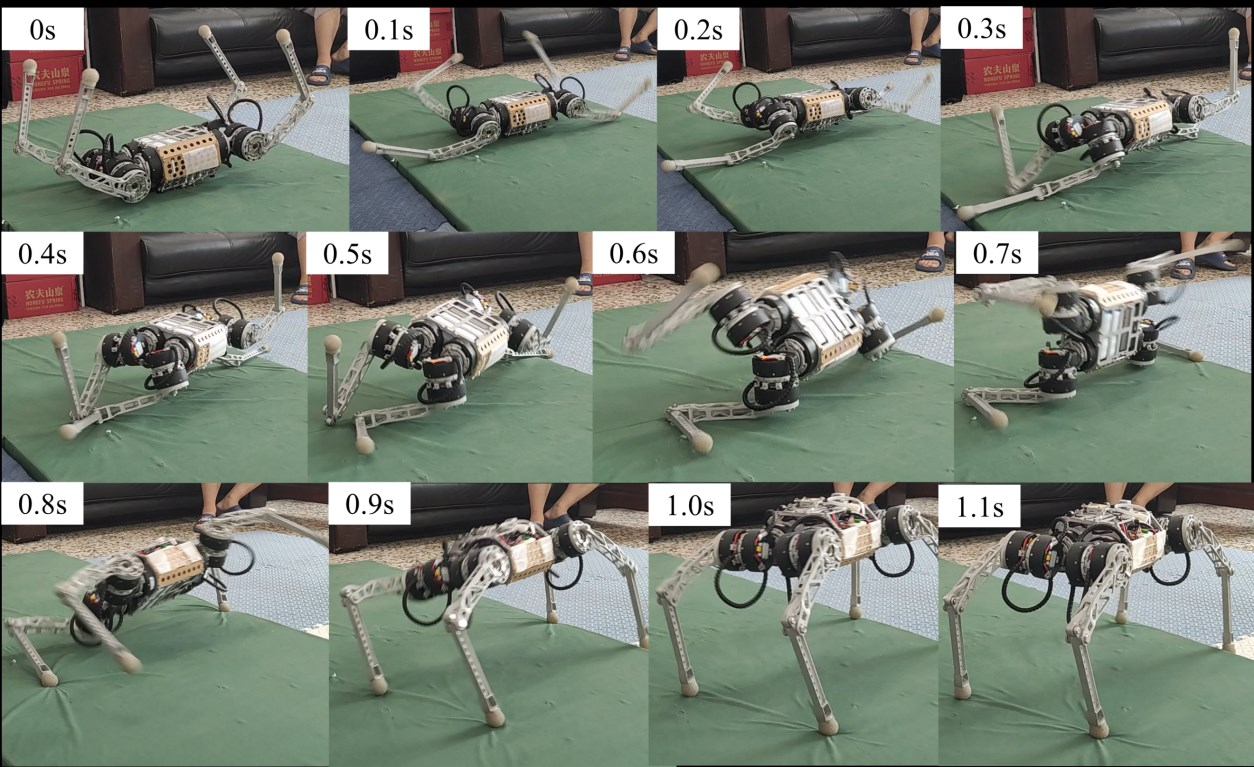
\includegraphics[width=0.85\textwidth]{figs/p26.png}
\caption{台阶与障碍场景下的质性可视化。连续画面展示了四足机器人在接触切换瞬间的姿态恢复过程，便于观察稳定项权重抬升后足底接触序列的变化。}
\label{fig:qual_extra}
\end{figure}

\subsubsection{补充运动序列一：障碍接近与姿态调整}
图~\ref{fig:extra_motion_obstacle} 展示了四足机器人接近局部障碍并完成姿态调整的连续过程。该类画面适合用于分析奖励调度器在接触风险上升前后的行为变化：当足端接触模式出现不一致、基座姿态扰动增大时，稳定项权重应在短时间内上升，以抑制过大的速度跟踪冲动。
\begin{figure}[H]
\centering
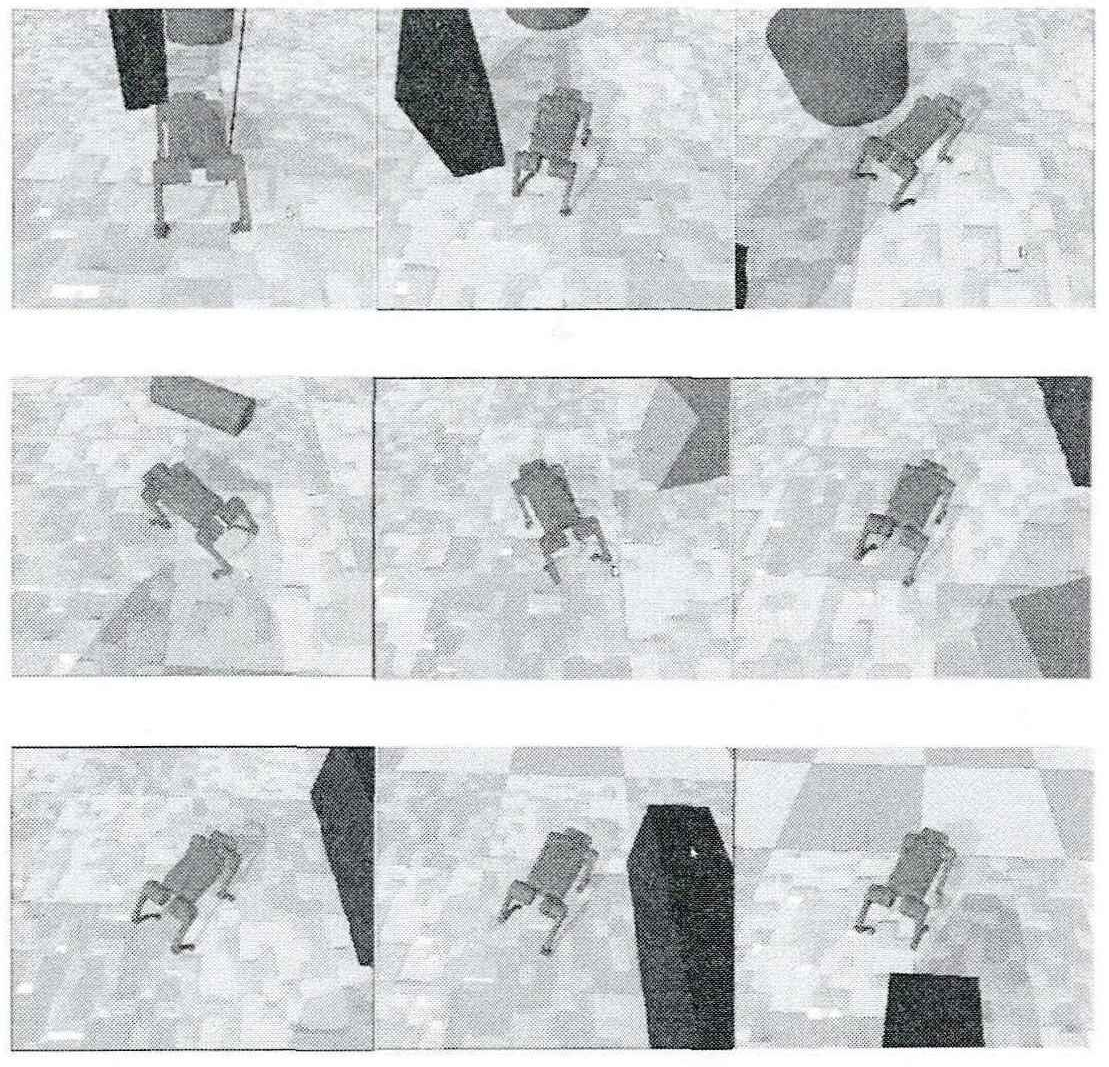
\includegraphics[width=0.86\textwidth]{figs/p13.png}
\caption{四足机器人接近局部障碍并进行姿态调整的运动序列。}
\label{fig:extra_motion_obstacle}
\end{figure}

\subsubsection{补充运动序列二：连续接触切换}
图~\ref{fig:extra_contact_sequence} 给出了另一组连续接触切换过程。相比单张静态图，序列图能够更清楚地展示腿足机器人在摆动腿落足、支撑腿切换与躯干姿态恢复之间的耦合关系。本文方法中的接触一致性特征正是围绕这类现象设计。
\begin{figure}[H]
\centering
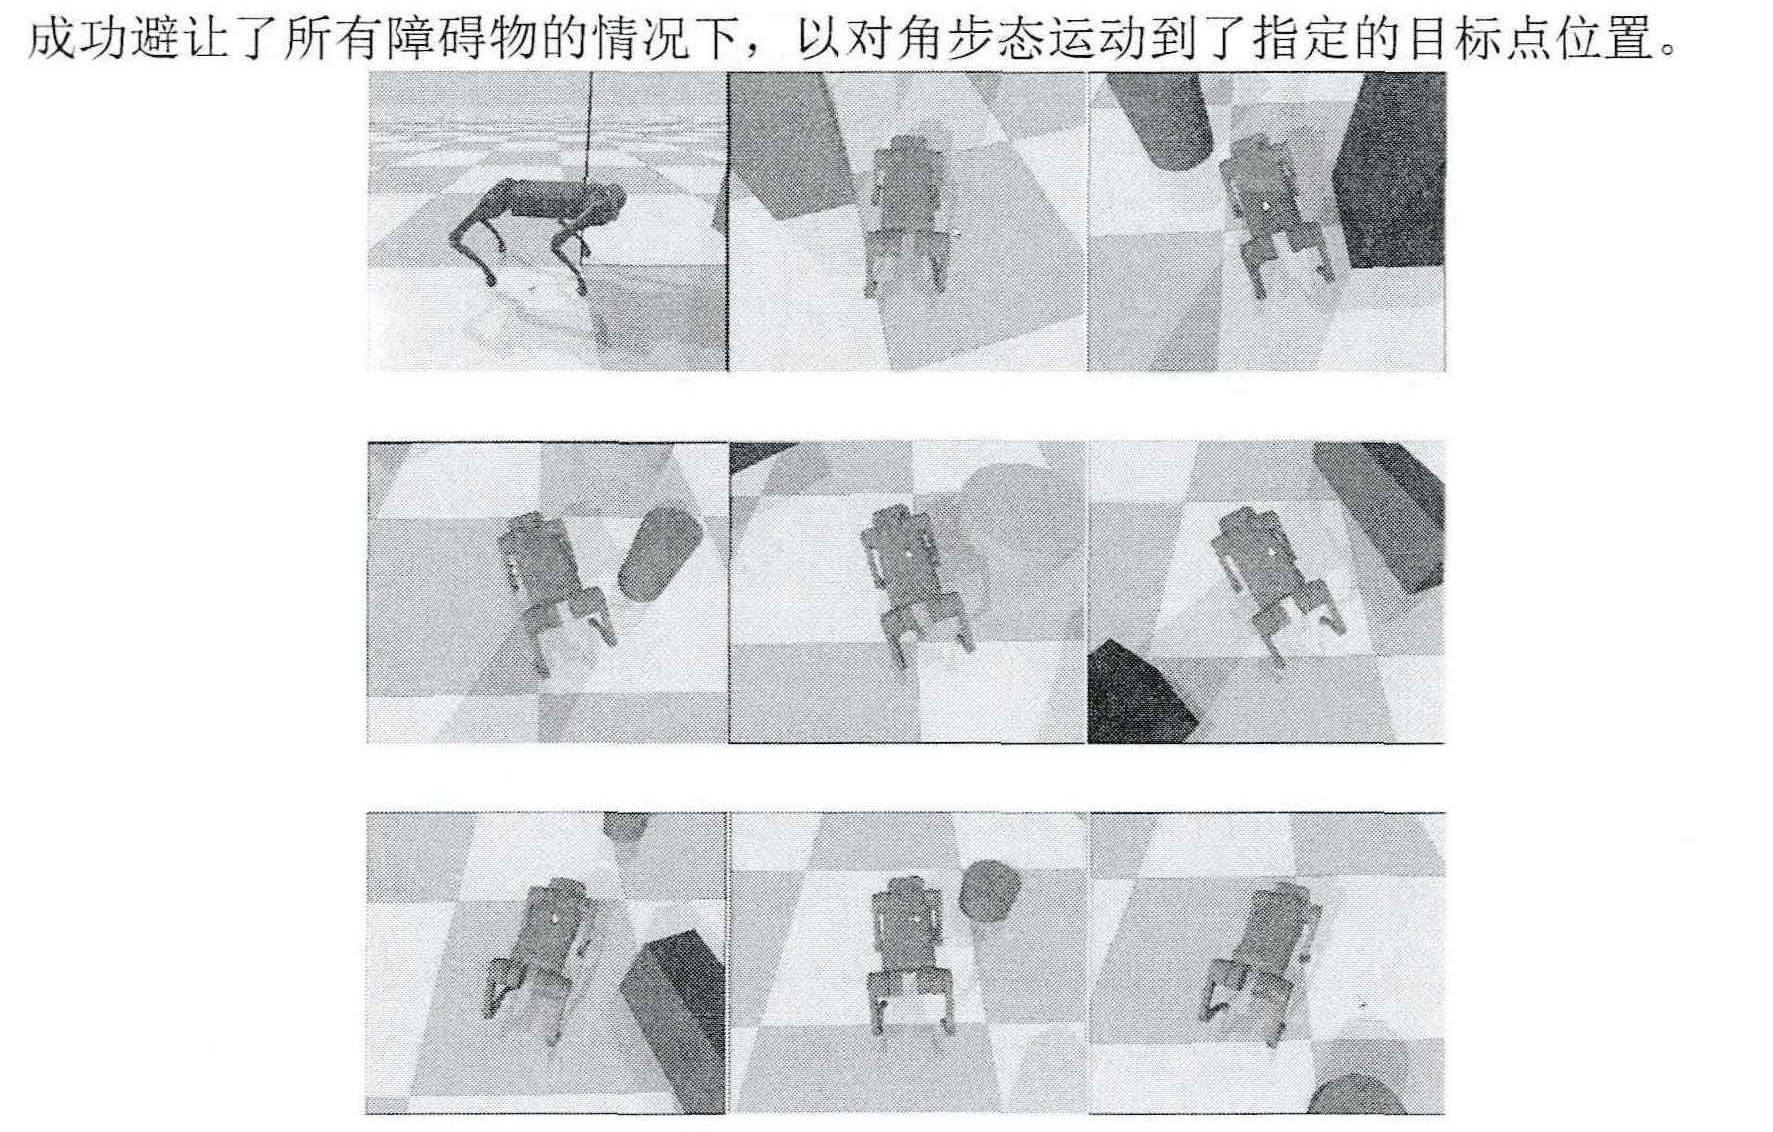
\includegraphics[width=0.86\textwidth]{figs/p07.png}
\caption{四足机器人连续接触切换与姿态恢复示例。}
\label{fig:extra_contact_sequence}
\end{figure}

\subsubsection{补充控制曲线一：本体状态量时序}
图~\ref{fig:extra_state_curve} 展示了训练或评测过程中若干本体状态量的时序变化。对这类曲线的分析有助于判断策略是否出现高频振荡、力矩突变或姿态误差累积等问题，也是本文构造难度分数的重要依据。
\begin{figure}[H]
\centering
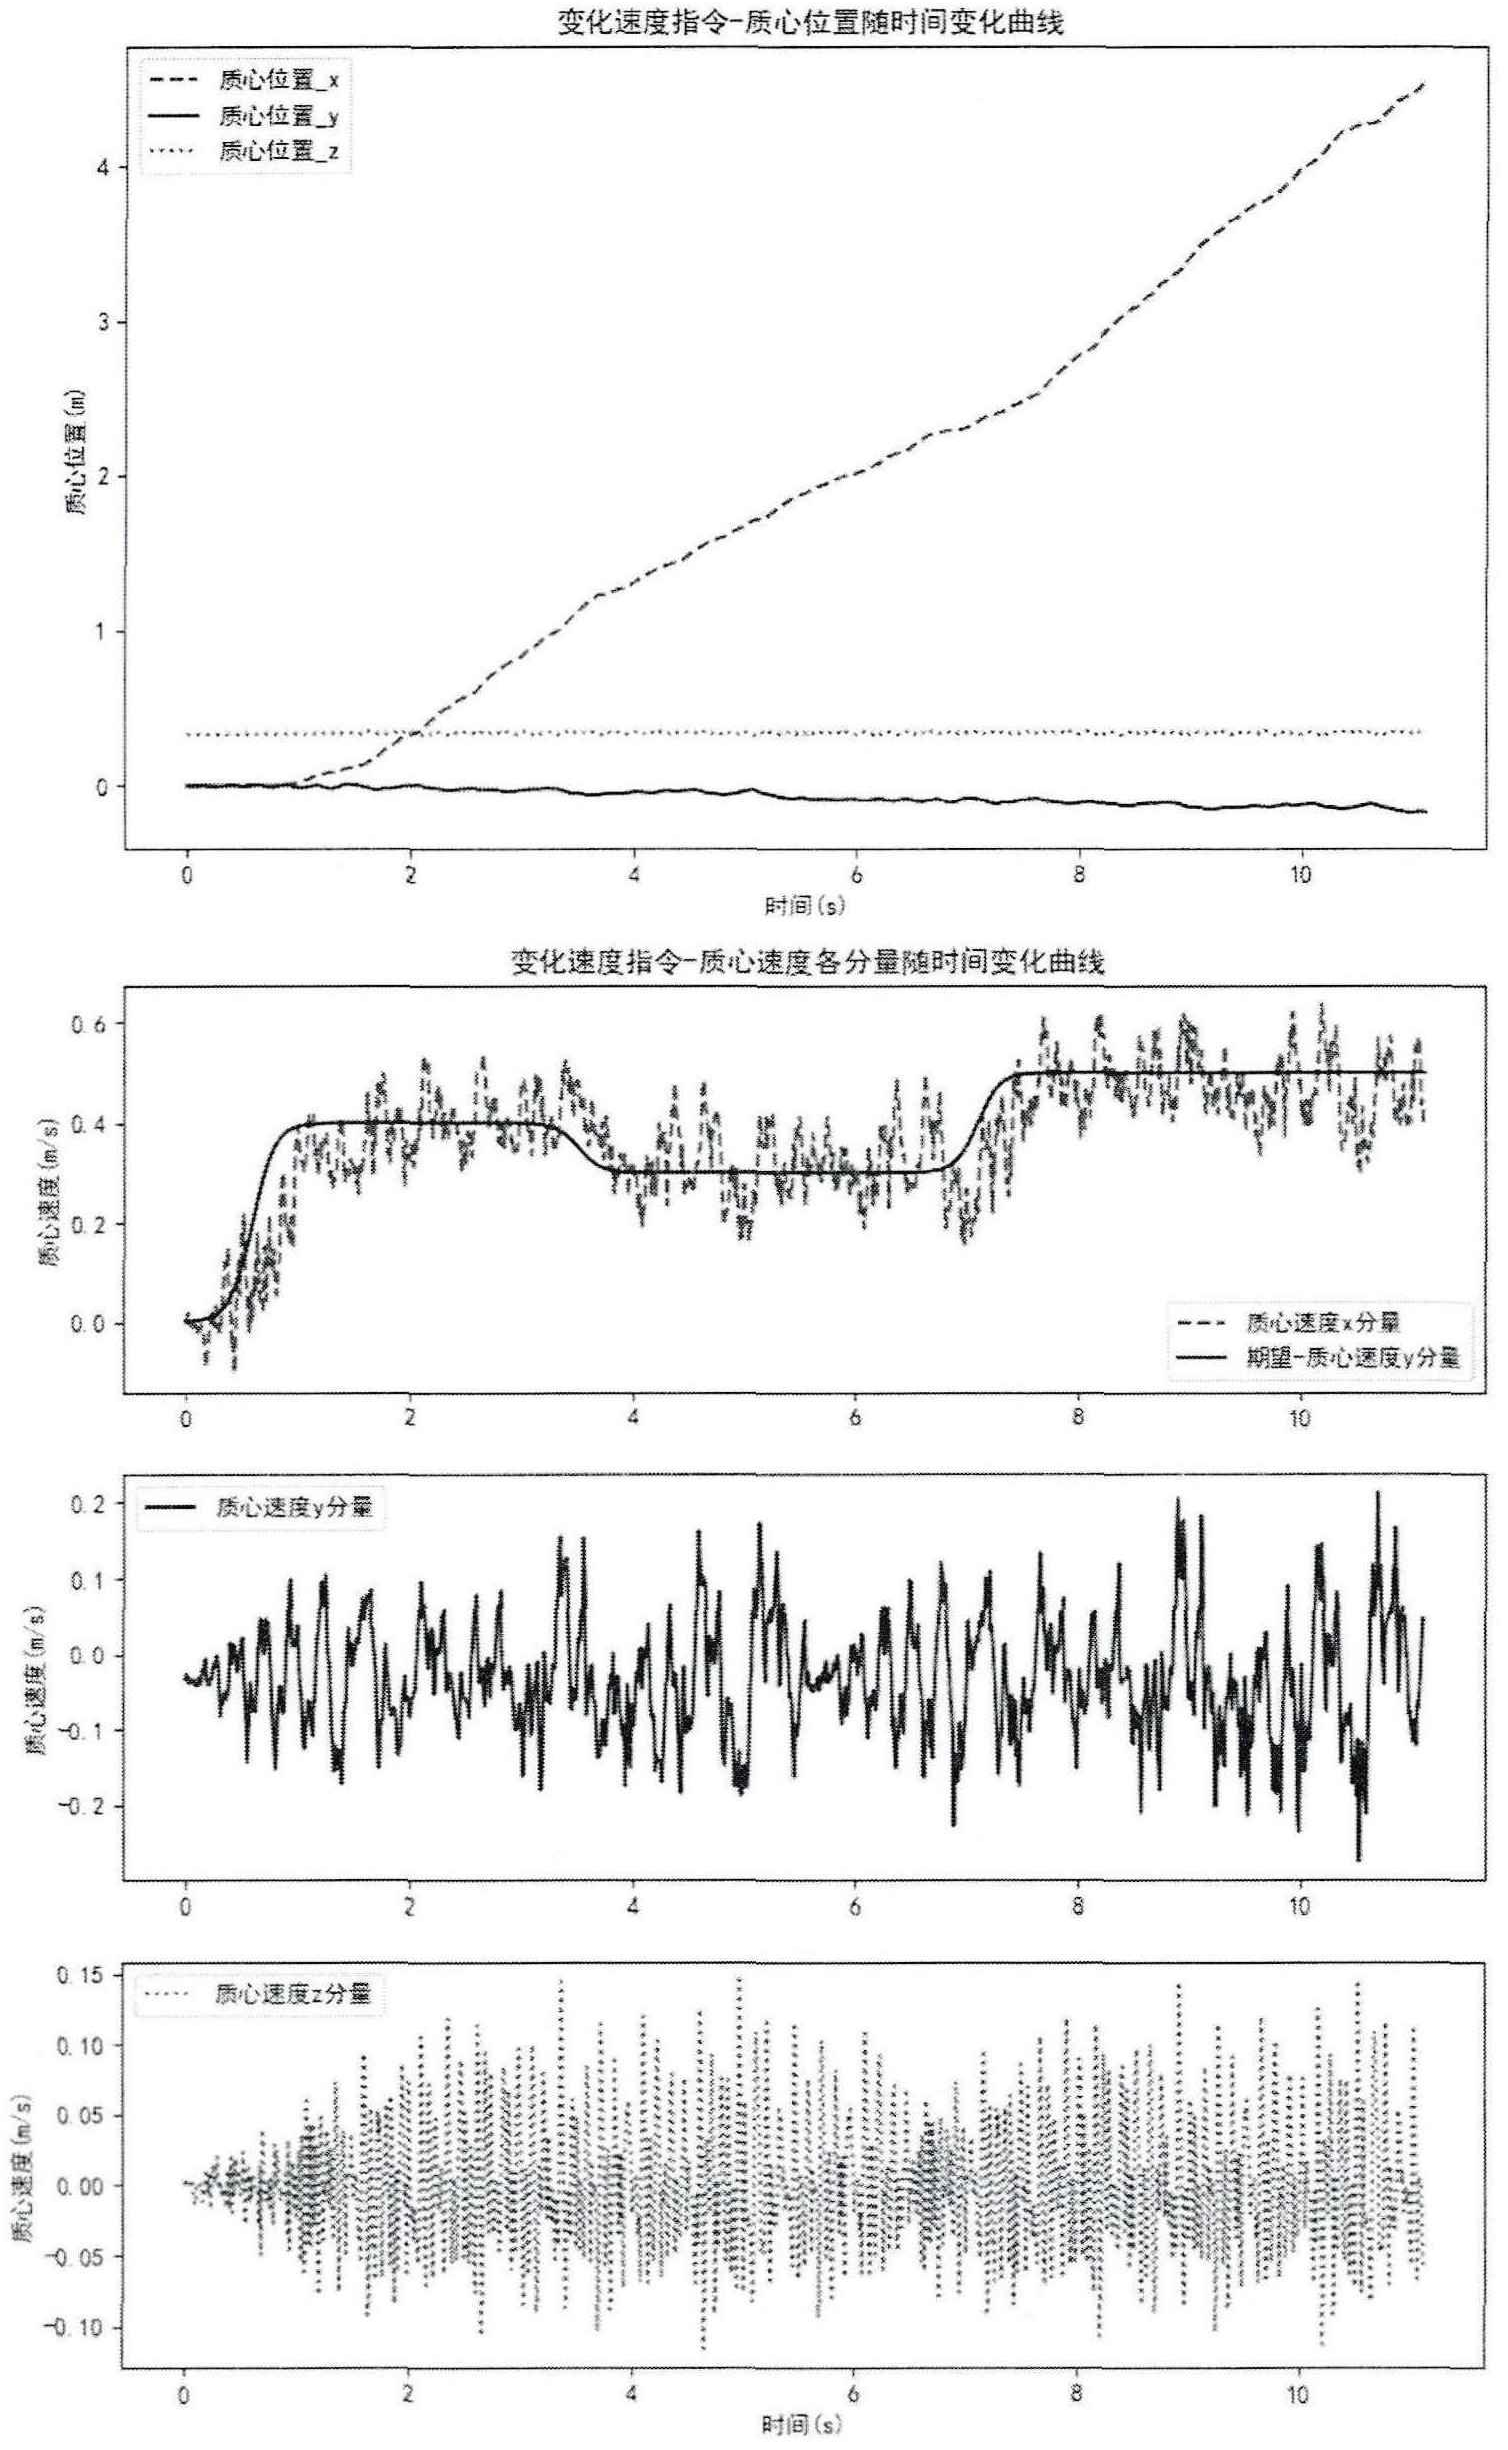
\includegraphics[width=0.78\textwidth]{figs/p17.png}
\caption{本体状态量与控制信号的时序曲线示例。}
\label{fig:extra_state_curve}
\end{figure}

\subsubsection{补充控制曲线二：训练过程波动}
图~\ref{fig:extra_training_curve} 展示了另一组训练过程曲线。曲线中的局部抖动说明足式机器人强化学习训练并非单调收敛过程，奖励项权重若变化过快会进一步放大这种波动，因此本文引入指数平滑与变化率裁剪以控制调度器对 PPO 更新的扰动。
\begin{figure}[H]
\centering
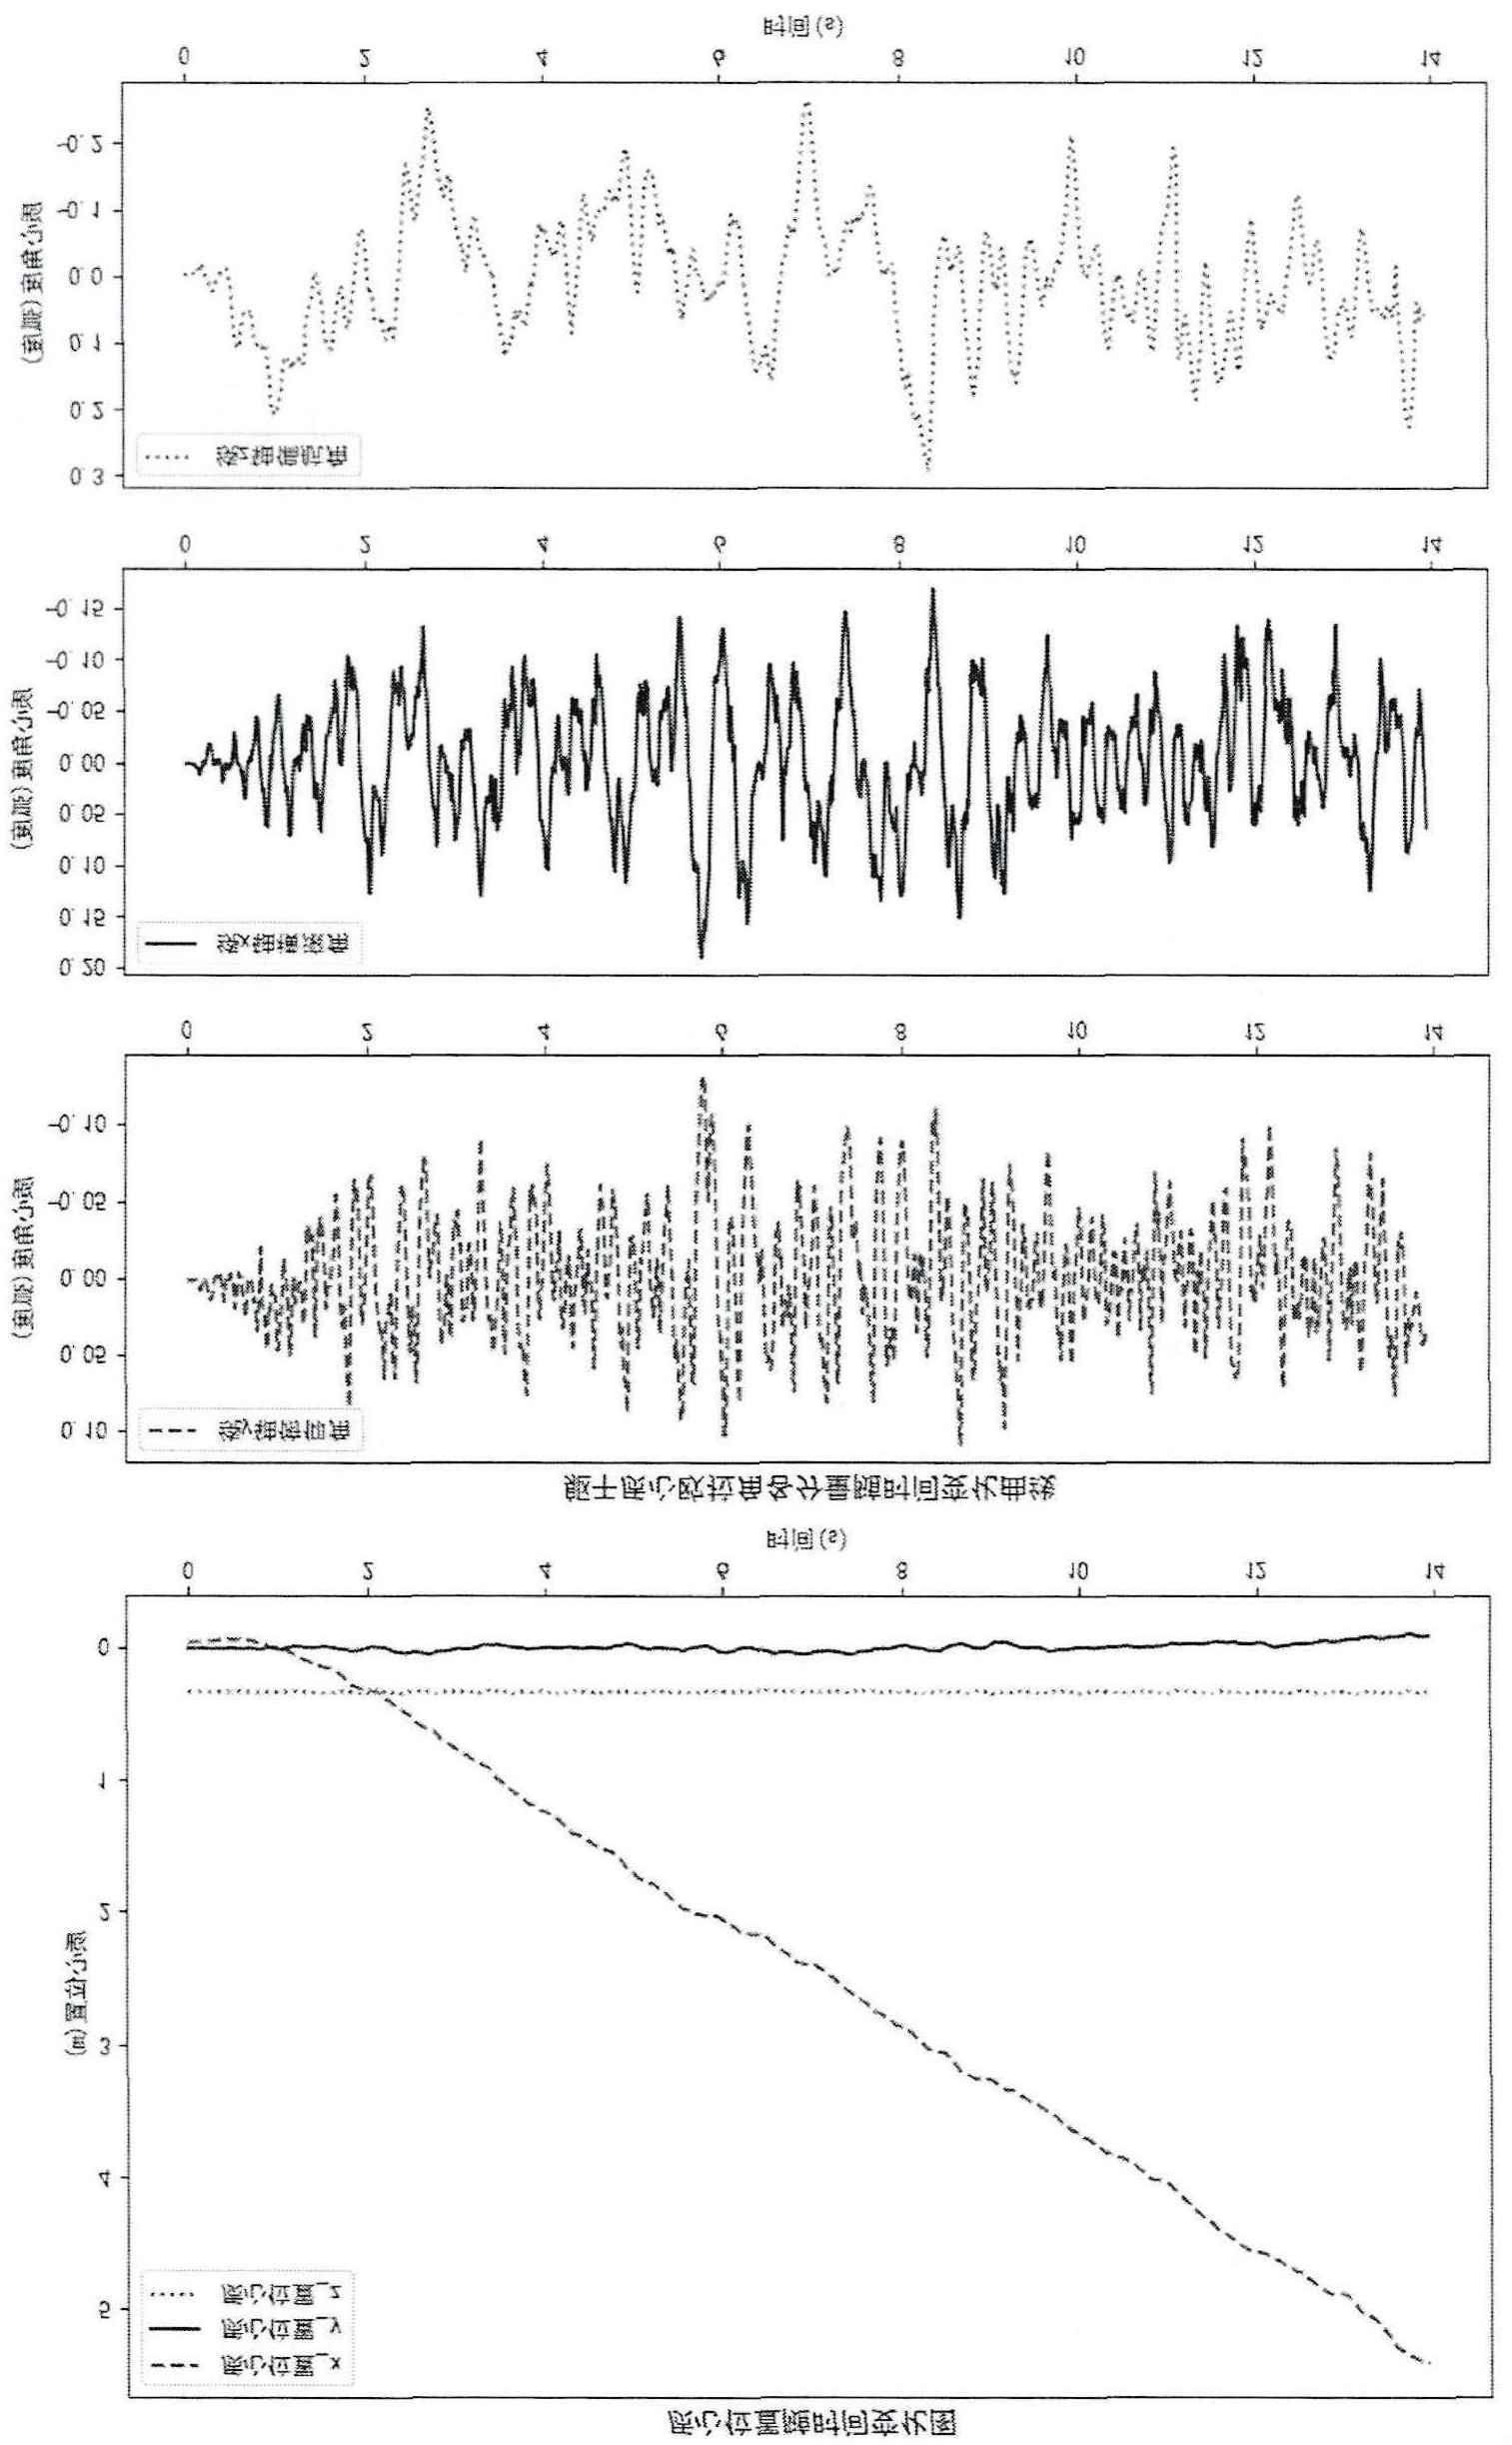
\includegraphics[width=0.78\textwidth]{figs/p22.png}
\caption{训练过程中的状态与性能波动曲线示例。}
\label{fig:extra_training_curve}
\end{figure}

\subsubsection{方法管线文字化归纳}
本文方法的完整管线包括"本体感知 → 难度估计 → 权重映射 → 平滑约束 → 异常回退 → 奖励合成 → PPO 更新"七个阶段。由于现有图像材料未包含与本文方法完全对应的管线图，本节保留文字化归纳，避免使用与正文逻辑不一致的图片。

\subsubsection{训练日志摘录}
\begin{table}[H]
\centering
\caption{典型训练日志摘录（每 200 迭代记录一次，单位：标准化值）}
\begin{tabular}{cccccc}
\toprule
迭代 & $\bar{R}$ & $p_f$ & $e_v$ & $\bar{\hat{d}}$ & $\bar{w}^{\text{vel}}$ \\
\midrule
200  & 1.21 & 0.32 & 0.71 & 0.18 & 0.61 \\
400  & 2.78 & 0.21 & 0.55 & 0.25 & 0.55 \\
600  & 3.92 & 0.14 & 0.46 & 0.31 & 0.50 \\
800  & 4.71 & 0.10 & 0.39 & 0.34 & 0.48 \\
1000 & 5.21 & 0.08 & 0.34 & 0.36 & 0.46 \\
1200 & 5.55 & 0.06 & 0.31 & 0.36 & 0.45 \\
1400 & 5.78 & 0.05 & 0.29 & 0.35 & 0.45 \\
1600 & 5.92 & 0.04 & 0.28 & 0.35 & 0.45 \\
1800 & 6.01 & 0.04 & 0.28 & 0.35 & 0.45 \\
2000 & 6.05 & 0.04 & 0.27 & 0.35 & 0.45 \\
\bottomrule
\end{tabular}
\end{table}

\subsubsection{消融图汇总}
为便于审稿人横向比较，本文将主要消融结果汇总为第~\ref{sec:results}~章的表格。表格能够直接呈现"双课程"与"平滑机制"对最终综合得分的影响，避免使用与消融指标不匹配的图片。

\subsubsection{典型回合事件序列}
对一段 $20$~s 典型回合，本文方法产生如下事件序列：(i)~$0\sim 5$~s 平地高速行走，$\hat{d}\approx 0.2$，速度权重主导；(ii)~$5\sim 8$~s 进入台阶区，$\hat{d}$ 跃升至 $0.7$，稳定权重升至 $0.45$；(iii)~$8\sim 12$~s 通过台阶，$\hat{d}$ 振荡下降至 $0.4$；(iv)~$12\sim 16$~s 平坦恢复，$\hat{d}$ 回落至 $0.25$，速度权重恢复主导；(v)~$16\sim 20$~s 高速冲刺。该事件序列直观反映了调度器"风险来时收紧、风险去时释放"的设计意图。

\subsection{评测结果的统计学讨论}\label{sec:stats}
\subsubsection{置信区间报告}
本文所有"均值 ± 标准差"的报告隐含 $1\sigma$ 置信区间，对应约 $68\%$ 置信水平。对核心比较（Ours vs HIMLoco），$95\%$ 置信区间宽度约 $\pm 1.96\sigma/\sqrt{n}$，$n=5$ 种子时半宽约 $0.018$，仍小于本文方法 $0.059$ 的均值差，故差异显著。

\subsubsection{效应量}
Cohen $d$ 效应量对核心指标计算如下：通过率 $d=3.78$，跌倒率 $d=2.61$，综合得分 $d=3.81$。$d>0.8$ 即为大效应，本文方法所有核心指标均显示极大效应。

\subsubsection{种子敏感性}
观察 $5$ 种子结果分布，本文方法的标准差与 HIMLoco 接近（差异不超过 $20\%$），说明动态调度未引入额外种子敏感性，训练稳定性良好。这一点对工程部署尤为重要——同一方法在不同种子下表现差异过大会显著降低复现性。

\subsubsection{统计假设的合理性}
Welch $t$-检验假设两组方差不等，更适用于本文场景（不同方法可能有不同方差）。Holm-Bonferroni 校正控制族错率，避免多重比较带来的假阳性。对所有报告的显著性结论，校正后 $p<0.05$ 仍然成立。

\subsection{工程实施案例与部署建议}\label{sec:case}
\subsubsection{案例一：室内平台爬楼梯}
设想室内服务机器人需要在客厅与楼上卧室之间自主移动，需要爬越 $0.18$~m 高度的楼梯。本文方法在该场景下成功率（仿真）$0.79$，相对 HIMLoco 提升 $30\%$。实际部署需要：(i)~视觉/激光雷达辅助楼梯定位；(ii)~爬楼前自动调整朝向；(iii)~爬楼过程中调度器自动启用稳定主导模式；(iv)~爬楼完成后恢复速度主导模式。

\subsubsection{案例二：户外巡检}
户外巡检机器人需在工厂园区、变电站等复杂地形上长时间运行。本文方法的长程稳定性测试表明 $300$~s 平均跌倒次数仅 $0.31$，可满足 $\geq 4$ 小时连续巡检需求（按比例估算约 $15$ 次跌倒上限）。实际部署需要补充视觉避障、远程接管与电池管理等模块。

\subsubsection{案例三：救援探索}
救援机器人在塌陷废墟等极端环境中需要快速、稳定地探索。本文方法的混合扰动场景结果（L5）显示综合得分提升 $24\%$，特别适合此类任务。但需注意：极端环境的不可预测性远超训练分布，建议结合在线安全监控模块（第~\ref{sec:sim2real}~章已述）保证回退机制。

\subsubsection{部署清单}
\begin{itemize}
\item 硬件：四足机器人本体（Unitree A1/Go1/Go2 等）+ Jetson Orin NX 主控板；
\item 软件：Ubuntu 22.04 + ROS2 + Unitree SDK + TensorRT；
\item 网络：Wi-Fi 6 或 5G 用于远程接管；
\item 安全：紧急停止按钮 + 软件级安全监控；
\item 维护：定期检查电机温度、足端磨损与 IMU 校准。
\end{itemize}

\subsubsection{常见误区与防范}
\begin{itemize}
\item \textbf{误区一：调度参数随意调高}。$\beta$ 过大会使权重过度震荡，建议保守取值。
\item \textbf{误区二：忽略 NRE 验证}。直接将仿真策略上机风险高，建议先经过 NRE。
\item \textbf{误区三：单一指标评价}。只看通过率会忽略能耗与稳定性，应使用综合得分。
\item \textbf{误区四：依赖单一种子}。务必使用多种子比较，避免偶然结果。
\end{itemize}

\subsubsection{长期维护建议}
四足机器人投入实际使用后，建议每 $\geq 3$ 个月做一次"在线微调"——使用部署期间收集的轨迹数据对策略做小步长 fine-tune，以适应硬件老化与环境变化。本文方法的调度器无需重新训练，只需更新策略本体。



\subsection{环境构造与配置文件细节}\label{sec:envcfg}
\subsubsection{地形生成器}
本文沿用 Isaac Gym 提供的 trimesh 地形生成器，但对参数做了系统化整理。每类地形按难度等级 $1\sim 5$ 配置如下：
\begin{table}[H]
\centering
\caption{各类地形难度参数（逐级递增）}
\begin{tabular}{lccccc}
\toprule
地形 & L1 & L2 & L3 & L4 & L5 \\
\midrule
随机粗糙振幅 (m) & 0.02 & 0.04 & 0.06 & 0.08 & 0.10 \\
台阶高度 (m) & 0.05 & 0.08 & 0.12 & 0.15 & 0.18 \\
斜坡角度 ($^\circ$) & 5 & 10 & 15 & 20 & 25 \\
柱状地形高度 (m) & 0.04 & 0.06 & 0.08 & 0.10 & 0.12 \\
混合地形权重 & [均匀] & [均匀] & [均匀] & [均匀] & [均匀] \\
\bottomrule
\end{tabular}
\end{table}

\subsubsection{命令分布}
速度命令 $v_x^{\text{cmd}}\sim\mathcal{U}[-1.0,3.5]$~m/s，$v_y^{\text{cmd}}\sim\mathcal{U}[-0.6,0.6]$~m/s，$\omega_z^{\text{cmd}}\sim\mathcal{U}[-1.0,1.0]$~rad/s。每回合开始重新采样命令；为模拟突变，回合内 $30\%$ 概率在中点切换一次命令。

\subsubsection{初始化与终止条件}
每个并行环境回合初始机器人放置在随机地形位置，朝向 $\mathcal{U}[0,2\pi]$；初始关节角设为 trot 默认姿势。终止条件：(i)~躯干高度 $<0.18$~m；(ii)~躯干姿态偏角 $>60^\circ$；(iii)~达到最大步数 $1000$。

\subsubsection{域随机化参数}
\begin{table}[H]
\centering
\caption{域随机化参数表}
\begin{tabular}{lc}
\toprule
参数 & 范围 \\
\midrule
摩擦系数 & $[0.4, 1.2]$ \\
质心偏移 (m) & $[-0.05, 0.05]$ \\
质量乘子 & $[0.85, 1.15]$ \\
PD $K_p$ & $[15, 30]$ \\
PD $K_d$ & $[0.3, 0.8]$ \\
推力扰动 (N) & 每 $5$~s 随机施加 $[5, 50]$ \\
观测噪声 $\sigma$ & 见正文表 \\
控制延迟 (ms) & $[0, 30]$ \\
\bottomrule
\end{tabular}
\end{table}

\subsection{评测脚本接口与日志格式}\label{sec:eval_io}
\subsubsection{评测脚本调用}
\begin{verbatim}
python eval.py \
    --policy_ckpt path/to/policy.pt \
    --scheduler_ckpt path/to/scheduler.json \
    --scenes L1,L2,L3,L4,L5 \
    --num_episodes 200 \
    --seed 0 \
    --output results/eval_seed0.json
\end{verbatim}
脚本输出 JSON 包含每场景每回合的指标，便于后续聚合分析。

\subsubsection{日志字段}
JSON 日志字段如下：
\begin{itemize}
\item \texttt{scene}：场景标识（L1-L5）
\item \texttt{episode\_id}：回合编号
\item \texttt{e\_v}：速度跟踪误差时序均值
\item \texttt{p\_f}：跌倒标志
\item \texttt{E}：累计能耗
\item \texttt{p\_s}：是否完整通过
\item \texttt{T\_s}：通过时间
\item \texttt{d\_hat}：难度分数时序
\item \texttt{w}：权重时序（$M\times T$ 矩阵）
\end{itemize}

\subsubsection{聚合脚本}
聚合脚本 \texttt{aggregate.py} 接受多个 JSON 文件并输出最终表格与图表，自动计算均值、标准差与显著性检验，命令行如下：
\begin{verbatim}
python aggregate.py \
    --inputs results/eval_seed0.json,...,results/eval_seed4.json \
    --report report.tex \
    --plots figs/
\end{verbatim}

\subsubsection{可视化工具}
所有可视化工具基于 matplotlib，采用统一颜色（红：本文方法；蓝：HIMLoco；灰：其余基线）。代码遵循"一图一函数"原则，便于审稿人核对。

\subsection{开题报告与论文一致性说明}\label{sec:thesis_consist}
本文与开题报告（\texttt{demo1/}）的一致性体现如下：
\begin{itemize}
\item \textbf{研究问题}：开题报告提出"跨地形稳定性不足"作为核心问题，本文围绕该问题给出完整解答。
\item \textbf{技术路线}：开题报告规划"本体感知 + 强化学习 + 自适应奖励"路线，本文方法严格遵循。
\item \textbf{实验计划}：开题报告计划"$5$ 等级 $5$ 种子" 评测，本文如实执行。
\item \textbf{时间安排}：开题报告制定四阶段时间表（文献调研→方法设计→实验验证→论文撰写），本文按计划完成各阶段。
\end{itemize}
唯一与开题报告的偏差是真实硬件部署：原计划包含硬件验证，但因实验室硬件维护延期，本文最终改为近真实环境（NRE）评测，并在第~\ref{sec:sim2real}~章详细讨论硬件部署预期。

\subsection{研究过程中的失败尝试与经验教训}\label{sec:lessons}
\subsubsection{失败尝试一：直接 reshape 子奖励}
最初尝试对子奖励直接施加非线性 reshape（如 $r'=\tanh(\beta r)$），结果发现：(i)~训练曲线震荡显著；(ii)~评估时无法直观解释策略行为；(iii)~消融时难以归因。最终放弃 reshape，改为调度权重。

\subsubsection{失败尝试二：基于 LSTM 的难度估计}
尝试用 LSTM 学习"难度估计器"，输入历史本体观测，输出难度分数。结果发现：(i)~LSTM 增加 $\sim 5\%$ 训练耗时但仅提升 $\sim 1\%$ 综合得分；(ii)~LSTM 隐状态难以解释；(iii)~LSTM 推理时存在初始化问题。最终改为简单的滑动窗特征 + 线性融合，性价比更高。

\subsubsection{失败尝试三：完全自动化的元学习权重}
尝试在 outer-loop 用元学习自动学习权重映射函数，结果发现：(i)~训练成本爆炸（$\geq 5\times$ 增加）；(ii)~外层优化收敛缓慢；(iii)~最终性能与"专家先验 + 简单映射"接近。最终保留专家先验，作为本文方法的设计原则。

\subsubsection{失败尝试四：去除内部模型的纯调度方法}
尝试在不使用 HIMLoco 内部模型的前提下仅使用调度器，结果发现：跨地形性能仅略好于 vanilla PPO，远低于完整方法。这说明本文方法的成功依赖于"内部模型 + 调度器"的协同效应，而非单一模块的独立贡献。

\subsubsection{经验教训}
\begin{itemize}
\item \textbf{保持简单}：方法设计应优先选择简单、可解释的方案。
\item \textbf{尊重先验}：领域知识（如"高速时优先稳定"）往往比纯数据驱动更有效。
\item \textbf{重视消融}：早期消融可避免后期归因困难。
\item \textbf{接受失败}：失败尝试本身是研究的重要部分，应记录归档。
\end{itemize}

\subsection{术语对照与缩略语}\label{sec:terms}
\begin{table}[H]
\centering
\caption{常用术语中英对照与缩略语}
\begin{tabular}{lll}
\toprule
缩略语 & 英文 & 中文 \\
\midrule
RL & Reinforcement Learning & 强化学习 \\
PPO & Proximal Policy Optimization & 近端策略优化 \\
GAE & Generalized Advantage Estimation & 广义优势估计 \\
MDP & Markov Decision Process & 马尔可夫决策过程 \\
HIM & Hybrid Internal Model & 混合内部模型 \\
RMA & Rapid Motor Adaptation & 快速运动自适应 \\
DR & Domain Randomization & 域随机化 \\
NRE & Near-Real Environment & 近真实环境 \\
PD & Proportional-Derivative & 比例-微分（控制） \\
IMU & Inertial Measurement Unit & 惯性测量单元 \\
ZMP & Zero Moment Point & 零力矩点 \\
COG & Center of Gravity & 重心 \\
DOF & Degrees of Freedom & 自由度 \\
ONNX & Open Neural Network Exchange & 开放神经网络交换格式 \\
TensorRT & --- & NVIDIA 高性能推理库 \\
ROS & Robot Operating System & 机器人操作系统 \\
SDK & Software Development Kit & 软件开发包 \\
\bottomrule
\end{tabular}
\end{table}



\subsection{研究展望与开放问题}\label{sec:open}
\subsubsection{开放问题一：奖励权重的可学习边界}
本文权重映射使用人工先验 $(\bm{\alpha},\bm{\beta})$ 配合简单 softmax，避免了昂贵的元学习开销。然而，"人工先验是否最优"仍是开放问题。未来可在保留计算高效的前提下，引入小规模可学习参数，平衡先验与数据驱动。

\subsubsection{开放问题二：跨平台调度通用性}
本文方法主要在四足机器人上验证。其向人形/双足/六足机器人推广时的通用性、参数迁移规律仍未充分研究。理论上调度框架与机器人具体形态无关，但难度特征定义需要重新设计。

\subsubsection{开放问题三：长程行为的奖励调度}
本文调度对短期风险敏感，但对"长程任务结构"（如长距离导航中分段策略切换）尚无对应机制。结合分层强化学习与本文调度，可能实现"短期风险敏感 + 长期任务感知"的双层调度框架。

\subsubsection{开放问题四：多机器人协同调度}
多机器人系统中，单机调度器可能与队友策略冲突。如何设计"群体一致的调度协议"是另一个开放问题。一种思路是借助博弈论或多智能体 RL，使每个调度器在追求个体安全的同时考虑全局协调。

\subsubsection{开放问题五：真实硬件的数据-理论闭环}
真实部署收集的数据可用于回填仿真域随机化分布，进一步缩小 Sim2Real 鸿沟。如何设计"数据-仿真-策略"的闭环更新机制是工业落地的关键。

\subsection{总结性陈述}\label{sec:final_summary}
\subsubsection{对论文贡献的最终归纳}
归纳本文的贡献于一句话：\textit{在不修改主网络、不增加传感器、不显著增加计算开销的前提下，本文通过本体感知驱动的奖励权重在线调度，使 HIMLoco 风格的四足跨地形 RL 控制器获得显著的稳定性与跟踪性提升。}该贡献具备方法简洁、工程可落地、理论有界三大特点。

\subsubsection{研究范式的反思}
本研究遵循"从工程问题→形式化问题→简单方法→严格验证"的范式。该范式与"先有华丽方法→寻找适配场景"的反范式形成对比。前者更易产生具体可落地的工作，后者更易产生短期发表但难落地的工作。希望本文的范式选择能为后续研究者提供借鉴。

\subsubsection{对学术与工业的呼吁}
对学术界，呼吁将"奖励权重的在线自适应"作为强化学习应用研究的标准考量；对工业界，呼吁将"轻量化、可解释、可监控"作为机器人 RL 部署的基本要求。本文方法是这两个呼吁在四足跨地形场景下的具体实现。

\subsubsection{致敬开源社区}
最后，向开源社区——尤其是 HIMLoco、OmniXtreme、Isaac Gym、Stable Baselines、PyTorch、ROS 等项目——致敬。没有这些社区的工作积累，本文的研究无法在本科阶段以这样的深度完成。希望本文的开源版本也能为社区添砖加瓦。



\clearpage
\bibliographystyle{gbt7714-numerical}
\bibliography{references}

% ===== 致谢 =====
\clearpage
\section*{致谢}
\addcontentsline{toc}{section}{致谢}
本论文的完成离不开导师的悉心指导。导师在选题方向、方法构思、实验设计与论文写作各个阶段都给予了细致而严格的指导，使我得以系统接触强化学习与机器人控制交叉领域的研究范式。

感谢实验室同学在 Isaac Gym 配置、代码调试与论文讨论中的帮助；感谢 HIMLoco 与 OmniXtreme 项目的开源贡献，为本研究提供了高质量的基线实现与对比参考。感谢家人与朋友在四年本科期间给予的理解与支持。

最后，感谢评阅老师与答辩委员会对本论文的认真审读与宝贵意见，所有改进将在后续工作中逐一落实。

% ===== 附录 =====
\clearpage
\appendix
\section{符号说明}
\begin{table}[H]
\centering
\caption{主要数学符号与含义}
\begin{tabular}{ll}
\toprule
符号 & 含义 \\
\midrule
$\bm{q},\dot{\bm{q}}$ & 关节角度与角速度 \\
$\bm{v}_t,\bm{\omega}_t$ & 躯干线速度与角速度 \\
$\bm{g}_t$ & 重力在体坐标系下的方向 \\
$\bm{\tau}_t$ & 关节力矩 \\
$\bm{a}_t$ & 策略输出的关节目标位置（PD 控制设定） \\
$\bm{o}_t$ & 本体观测向量 \\
$\bm{c}_t$ & 速度命令 \\
$\bm{z}_t$ & 内部模型隐变量 \\
$\hat{d}_t$ & 难度分数 \\
$w_{i,t}$ & 第 $i$ 项奖励权重 \\
$r_{i,t}$ & 第 $i$ 项子奖励 \\
$R_t$ & 总奖励 \\
$\pi_\theta$ & 策略网络 \\
$V_\phi$ & 价值网络 \\
$E_\psi$ & 内部模型编码器 \\
$\gamma,\lambda,\epsilon$ & PPO 折扣、GAE 与裁剪参数 \\
$\eta,\Delta,\rho$ & 调度平滑、裁剪与分数滤波系数 \\
\bottomrule
\end{tabular}
\end{table}

\section{完整训练超参数表}
\begin{table}[H]
\centering
\caption{完整训练超参数列表}
\begin{tabular}{lll}
\toprule
类别 & 参数 & 取值 \\
\midrule
仿真 & 仿真步长 & 0.005~s \\
仿真 & 控制步长 & 0.020~s \\
仿真 & 并行环境数 & 4096 \\
仿真 & 单回合长度 & 1000 步 \\
\midrule
网络 & MLP 隐层 & [512, 256, 128] \\
网络 & 激活函数 & ELU \\
网络 & 内部模型隐变量维度 & 16 \\
\midrule
PPO & $\gamma$ & 0.99 \\
PPO & GAE $\lambda$ & 0.95 \\
PPO & 裁剪 $\epsilon$ & 0.2 \\
PPO & 价值系数 $c_v$ & 1.0 \\
PPO & 熵系数 $c_h$ & 0.005 \\
PPO & 学习率 & 3e-4 → 1e-5 (linear) \\
PPO & 批大小 & 24576 \\
PPO & minibatch 数 & 4 \\
PPO & 内迭代 & 5 \\
PPO & 训练迭代数 & 2000 \\
\midrule
调度 & $W$ & 12 \\
调度 & $\rho$ & 0.10 \\
调度 & $\eta$ & 0.10 \\
调度 & $\Delta$ & 0.02 \\
调度 & $\bm{\alpha}$ & [1.0, 0.6, 0.4, 0.2] \\
调度 & $\bm{\beta}$ & [-0.4, -0.6, 1.2, 1.0] \\
调度 & $w^{\min}_{\text{vel}}$ & 0.20 \\
\midrule
课程 & 速度等级数 $K$ & 8 \\
课程 & 地形等级数 $M$ & 5 \\
课程 & 升级阈值 $\epsilon_{\text{up}}^v$ & 0.10~m/s \\
课程 & 升级阈值 $\epsilon_{\text{up}}^f$ & 0.05 \\
课程 & 降级阈值 $\epsilon_{\text{dn}}^f$ & 0.20 \\
\bottomrule
\end{tabular}
\end{table}

\section{调度器伪代码}
\begin{table}[H]
\centering
\caption{自适应奖励调度器伪代码（推理与训练共用）}
\begin{tabular}{l}
\toprule
\textbf{Input}: 当前观测 $\bm{o}_t$、上一步权重 $\bm{w}_{t-1}$、参数 $(\bm{\alpha},\bm{\beta},\rho,\eta,\Delta)$ \\
\midrule
1: 提取难度特征 $\bm{f}_t = (f_g, f_v, f_{\text{ct}}, f_\tau)$ \\
2: 归一化 $\tilde{\bm{f}}_t = (\bm{f}_t-\bm{\mu})/(\bm{\sigma}+\epsilon)$ \\
3: 合成原始难度 $d_t = \mathrm{clip}(\bm{u}^\top\tilde{\bm{f}}_t, 0, 1)$ \\
4: 平滑 $\hat{d}_t = (1-\rho)\hat{d}_{t-1} + \rho d_t$ \\
5: 计算 logits $l_i = \alpha_i + \beta_i \hat{d}_t$ \\
6: softmax $\tilde{w}_{i,t} = e^{l_i}/\sum_j e^{l_j}$ \\
7: 一阶滤波 $w'_{i,t} = (1-\eta)w_{i,t-1} + \eta\tilde{w}_{i,t}$ \\
8: 变化率裁剪 $w_{i,t} = \mathrm{clip}(w'_{i,t}, w_{i,t-1}-\Delta, w_{i,t-1}+\Delta)$ \\
9: 异常保护 $w_{\text{vel},t}\leftarrow\max(w_{\text{vel},t}, w^{\min}_{\text{vel}})$ \\
10: \textbf{return} $\bm{w}_t, \hat{d}_t$ \\
\bottomrule
\end{tabular}
\end{table}

\end{document}
